\documentclass[9pt,twocolumn,twoside]{rilabRxiv}
% Use the documentclass option 'lineno' to view line numbers
\setlength{\marginparwidth}{2cm}
\usepackage[textsize=tiny,colorinlistoftodos]{todonotes} % comments in margins
\definecolor{cornflowerblue}{rgb}{0.39, 0.58, 0.93}
\usepackage{blindtext}
\usepackage{nameref}
\usepackage{textcomp} % for \textdegree
\usepackage{newunicodechar}
\newunicodechar{≥}{\ensuremath{\geq}}
\newunicodechar{≤}{\ensuremath{\leq}}
\newunicodechar{–}{--}
\newunicodechar{—}{---}
\raggedbottom
\usepackage{booktabs}
\usepackage{afterpage}
\usepackage{pdflscape}
\usepackage{longtable}
\usepackage{tabularx}
\usepackage{array}
\newcolumntype{Y}{>{\raggedright\arraybackslash}X}
\usepackage{multirow}
\usepackage{makecell}
\usepackage{array}
\usepackage{threeparttable}

%%%%%%%Add comments in color
\newcommand{\ms}[1]{{\small \textcolor{green}{#1}}}
\newcommand{\citex}[1]{{\small \textcolor{red}{CITE(#1)}}}
\newcommand{\X}{{\textcolor{red}{X}}}
\newcommand{\mex}{\textit{mexicana}\xspace}
\newcommand{\invfour}{\textit{Inv4m}\xspace}
\newcommand{\fdrgt} {$\textrm{\textit{FDR}} > 0.05$}
\newcommand{\fdreq} {$\textrm{\textit{FDR}} = 0.05$}
\newcommand{\fdrls} {$\textrm{\textit{FDR}} < 0.05$}
\newcommand{\parv}{\textit{parviglumis}\xspace}
\newcommand{\arabidopis}{\textit{Arabidopsis}\xspace}

\newcolumntype{b}{X}
\newcolumntype{s}{>{\hsize=.5\hsize}X}

% Set supplement numbers to S and start counting newly
\newcommand{\beginsupplement}{%
    \setcounter{table}{0}%
    \renewcommand{\tablename}{}%  % <-- 1. Make the word 'Table' blank
    \renewcommand{\thetable}{S\arabic{table} Table}%  % <-- 2. Include ' Table' after the number
    \setcounter{figure}{0}%
    \renewcommand{\figurename}{}%  % <-- Make the word 'Figure' blank for consistency
    \renewcommand{\thefigure}{S\arabic{figure} Fig}%  % <-- Include ' Figure' after the number
}

\usepackage{CJKutf8}
% \begin{CJK}{UTF8}{min}
% \verb|¯\_(ツ)_/¯|
% \end{CJK}

\title{The Sorghum Lipid Database (SoLD): population-scale lipidomics linking environmental and genetic variation in the Sorghum Association Panel}

\author[$1$,$2$,*]{Nirwan Tandukar}
\author[$1$]{Ruthie Locklear}
\author[$3$]{Richard Boyles}
\author[$4$]{Zach Brenton}
\author[$5$]{Katherine Louie}
\author[$1$,*]{Rubén Rellán-Álvarez}
\affil[$1$,*]{Department of Molecular and Structural Biochemistry, N.C. Plant Sciences Initiative, North Carolina State University, Raleigh, NC, USA.}
\affil[$2$]{Genetics and Genomics Program, North Carolina State University, Raleigh, NC, USA}
\affil[$3$]{Department of Plant and Environmental Sciences, Clemson University, Clemson, SC, USA}
\affil[$4$]{Carolina Seed Systems, Darlington, South Carolina}
\affil[$5$]{Joint Genome Institute, Department of Energy, California, USA}

\keywords{Sorghum Association Panel, Lipidomics, Genome-wide Association Studies, Triglycerides, Phospholipids, Cold stress, Nutrient stress}

\runningtitle{Sorghum Lipid Database (SoLD): a database curation
for lipid information for Sorghum Association Panel} % For use in the footer

%% For the footnote.
%% Give the last name of the first author if only one author;
\runningauthor{Tandukar}
%% last names of both authors if there are two authors;
% \runningauthor{FirstAuthorLastname and SecondAuthorLastname}
%% last name of the first author followed by et al, if more than two authors.
\runningauthor{Tandukar \textit{et al.}}

%%% Abstract %%%%%%%%%%%%%%%%%%
\begin{abstract}
Sorghum (\textit{Sorghum bicolor}) is a climate-resilient crop whose acclimation to nutrient limitation and low temperature likely involves extensive lipidome reconfiguration. Lipids are key membrane components, carbon and energy stores, and mediators of stress signaling, yet population-scale lipidomics data for sorghum are limited. We present the Sorghum Lipid Database (SoLD), a curated lipidomics resource from the Sorghum Association Panel grown under two field regimes, (i) a nutrient-sufficient with usual planting date environment (control) and (ii) a low-input treatment with reduced nitrogen and phosphorus, earlier planting, and no application of insecticides, herbicides, or pesticides (low-input). Using high-resolution LC--MS, we quantified 266 lipid species and found the lipidome broadly similar across trials, with four low-input-associated signatures relative to control, (i) depletion of sulfoquinovosyldiacylglycerol, (ii) triacylglycerol enrichment, (iii) phospholipid redistribution centered on phosphatidylserine, and (iv) a shift in the lysophosphatidylcholine-to-lysophosphatidylethanolamine ratio. Analyses of lipid chemical space and lipid ontology enrichment supported these compositional changes. Genomic heritability was near zero under control and 0.170 under low input, reflecting more genetic variance rather than less experimental noise. GWAS of lipid species, class sums, and class ratios recovered loci that were largely trial-specific, with candidate genes assigned by linkage disequilibrium with the peak rather than by physical distance, and prioritized both by ontology terms passing an LD-aware permutation null and by mapping onto lipid reaction branches. Control-associated loci were enriched for tyrosine catabolism and oxidative-stress functions, whereas low-input-associated loci were enriched for nutrient transport and signaling, sphingolipid metabolism, and jasmonate-related regulation, and included a chromosome~3 block carrying two LOW PHOSPHATE ROOT homologues. Thus, SoLD provides a framework connecting sorghum lipid diversity with environmental and genetic variation. All information regarding the database and the experiment is freely accessible through a Shiny application: \url{https://nirwan.shinyapps.io/SAP-Lipidomics-Database/}. The database enables users to move from lipid-class to individual molecular species and associated candidate loci, for hypothesis generation, comparative analyses, and prioritization of targets for functional validation.




\end{abstract}

\setboolean{displaycopyright}{true}

\usepackage{hyperref}

\begin{document}

\maketitle
\thispagestyle{firststyle}
%\firstpagefootnote
\correspondingauthoraffiliation{
Department of Molecular and Structural Biochemistry, N.C. Plant Sciences Initiative, North Carolina State University, Raleigh, NC, USA.
E-mail: ntanduk@ncsu.edu, rrellan@ncsu.edu}
\vspace{-11pt}%

\setboolean{displaylineno}{false}
\ifthenelse{\boolean{displaylineno}}{\linenumbers}{}

\section{Introduction}

Plants routinely face environmental stresses that limit yield, such as nutrient limitation and low temperature. Nutrients such as nitrogen (N) and phosphorus (P) deficiencies are important for research because they restrict overall growth, nutrient allocation, and developmental plasticity, while low temperature disrupts cell membrane fluidity, metabolism, and yield \citep{Schluter2012, Silveira2018, Emendack2021, Ding2019, Guo2025}. Lipids are central to these environmental responses as cell membrane components, carbon and energy stores, and precursors of signaling molecules. Stress-driven lipid remodeling can alter membrane stability, photosynthetic capacity, storage-lipid abundance, and lipid-derived signaling \citep{Bohn2007, Siebers2015, Hou2016, Rawat2021, Li2020, Bhattacharya2022, Xu2025}. Under P limitation, plants usually replace phospholipids with non-P galactolipids and sulfolipids, including digalactosyldiacylglycerol (DGDG) and sulfoquinovosyldiacylglycerol (SQDG). Cold stress can shift acyl-chain composition, phospholipid turnover, and triacylglycerol (TG) accumulation \citep{Essigmann1998, Hartel2000, Jouhet2004, KellyDormann2002, Tan2018, Pfaff2020, Yan2025, Zhang2020}. These lipid responses are followed by nutrient and stress-regulatory pathways. An example includes the SPX-domain proteins, which regulate phosphate signaling through PHR-centered networks \citep{Lv2014SPX4}. Similarly, nitrate transporters such as NRT2 and NPF mediate N acquisition and allocation, and sulfate transporters influence plastid sulfur supply for sulfolipid metabolism \citep{Lupini2016NAR2, Sorgona2011Nitrate, Xia2015NPF24, Chen2019SULTR3}. In conjunction, lipid-remodeling enzymes, including non-specific phospholipases, DGATs, and SDP1-like lipases, mediate phospholipid turnover, DG production, and TG synthesis and mobilization \citep{Bose2021NPC, Ngo2019NPC, Tan2018, Kelly2011SDP1L, Yen2008DGAT}. However, population-scale lipidomics resources linking lipid remodeling, nutrient-stress, and natural genetic variation remain scarce in crops, particularly in sorghum.

Sorghum is a stress-resilient cereal crop with large genetic diversity. The Sorghum Association Panel (SAP) is a collection of sorghum lines with substantial genomic variation that captures broad botanical, geographic, and genetic diversity \citep{Casa2008CommunityResourcesSorghum, Boatwright2022}. This makes it ideal for studying natural variation due to environmental stresses. For lipidomics, however, population-scale interpretation requires careful data processing and annotation. LC–MS lipidomics can be affected by run-order drift, instrumental batch effects, and field-layout artifacts, while lipid annotation and naming can vary across studies. Here, we have used a QC-based normalization method, SERRF; spatial correction methods, SpATS; and a spectral annotation database, GNPS, that improve reproducibility and biological interpretation \citep{Fan2019, RodriguezAlvarez2018, Wang2016GNPS, Molenaar2019}.

A second challenge in population-scale lipidomics linked to GWAS is interpreting large candidate-gene sets. GWAS across many lipid species, class sums, and class ratios can yield hundreds to thousands of nearby genes, but LD-assigned genes are not independent. A single association can tag multiple neighboring genes, including tandem arrays with similar annotations, so standard gene-level enrichment can misinterpret one locus as pathway-level evidence. This issue led to GWAS-specific gene-set and interval-enrichment tools such as INRICH, SNP2GO, and Gowinda, which adjust for LD, candidate-SNP structure, or gene-level biases \citep{Lee2012INRICH,Szkiba2014SNP2GO,Kofler2012Gowinda}. Here, we extend this approach by testing Gene Ontology (GO) enrichment against an LD-aware interval-permutation null and by distinguishing terms supported by multiple independent genomic intervals from those driven by single annotated loci.

Here, we present the Sorghum Lipid Database (SoLD), a curated lipidomics and GWAS resource for the SAP. Leaf samples collected between the V6 and V8 stages were profiled under two field regimes: a control environment (CTL), grown in 2019 with sufficient nutrients and standard planting, and a low-input regime (LIN), grown in 2022 with reduced N and P, earlier planting to impose early-season cold-associated stress, and minimal chemical management, including no insecticide, herbicide, or pesticide application. Since CTL and LIN were grown in different field years, we interpret their contrasts conservatively as between-trial differences rather than direct causal treatment effects. 

We combine LC--MS lipidomics, compositional analysis, lipid ontology, GWAS of individual species and class-level traits, LD-aware GO enrichment, LINEX-based reaction mapping, and an interactive Shiny application. This framework identifies four major LIN-associated lipid signatures: SQDG depletion, TG enrichment, PS-centered phospholipid redistribution, and altered LPC/LPE balance. It also prioritizes candidate functions linked to nutrient acquisition, DG--TG cycling, phospholipid turnover, sphingolipid metabolism, and stress-associated membrane remodeling, including representative loci such as DGAT1 (\texttt{SORBI\_3010G170000}) for TG accumulation, a SULTR3-family sulfate transporter (\texttt{SORBI\_3006G244000}) for SQDG-related sulfur supply, and an SPX-domain phosphate-status (\texttt{SORBI\_3001G028500}) candidate. Together, SoLD provides a resource for exploring sorghum lipid variation, candidate loci, and accessions for future validation. The interactive SoLD Shiny application enables exploration of all datasets and results and is available at \url{https://nirwan.shinyapps.io/SAP-Lipidomics-Database/}.

\section{Results}

\subsection*{QC and normalization yielded comparable LC-MS performance across conditions}

We profiled early-stage lipids from SAP grown in two field conditions defined earlier. The workflow (Supplementary~\ref{fig:suppfig_s1_workflow}) comprised tissue collection and extraction, high-resolution LC-MS lipidomic profiling, GNPS-assisted lipid annotation, post-acquisition data correction with SERRF and SpATS \citep{Fan2019, RodriguezAlvarez2018}, and data dissemination via the SoLD Shiny app (\url{https://nirwan.shinyapps.io/SAP-Lipidomics-Database/}).

Run-order quality control showed stable analytical performance (Supplementary~\ref{fig:suppfig_s2_qc}A--B), with the total ion current (TIC) and the summed signal intensity per sample meeting expected values across system checks, internal standards, and blanks. TIC variability among QC samples was low (7.5\% CV for CTL and 6.0\% CV for LIN). SERRF normalization improved technical precision, reducing median QC-RSD from 3.6\% to 2.0\% in CTL and from 1.6\% to 0.3\% in LIN. The proportion of features with QC-RSD below 30\% rose from 75.7\% to 94.1\% and from 77.3\% to 89.3\% respectively (Supplementary~\ref{fig:suppfig_s2_qc}C--D).

PCA of normalized data showed tighter sample clustering than unprocessed data (Supplementary~\ref{fig:suppfig_s2_qc}E--F). After spatial correction, the leftover variation in MGDG(18:3/18:3) is scattered randomly across the field rather than forming rows, columns, or patches, indicating that position in the field no longer drives the signal (Supplementary~\ref{fig:suppfig_s2_qc}G--H). Thus, the post-correction lipid signal distributions remained similar across cohorts, and the adjusted values was used for all subsequent analyses.

\subsection*{Genotypic lipid variation is largely independent of botanical race, and heritable variation is confined to LIN}

SAP is structured by botanical race and geographic origin \citep{Casa2008CommunityResourcesSorghum, Boatwright2022}. Next, we tested whether lipid variation is affected by race or marker-based genetic clusters ($K=6$). Using Kruskal–Wallis with BH correction within trials (Supplementary Table~S1), we found little association. No lipid-class sum was significant for race in either trial. The genetic cluster was significant only for PS under LIN ($q=1.16\times10^{-6}$, $\varepsilon^2=0.104$; Fig.~\ref{fig:fig1_population_structure}). PS is carried by a single species under LIN, PS(18:0/18:2), so the class sum and that species are the same measurement. The same class-level test under CTL, where PS is carried by two species, was not significant ($\varepsilon^2=0.020$, $q=0.358$). Furthermore, none of the species-level tests were significant under CTL, and nine were significant under LIN, eight of them by genetic cluster alone and one, 11,14,17-eicosatrienoic acid, by both genetic cluster and botanical race (Table~\ref{tab:species_ancestry}; Supplementary Table~S2 (per-species structure and $h^2$)). PCA of class composition likewise showed minimal structure, with groupings explaining $\le$1.6\% of variation (Supplementary~\ref{fig:suppfig_s3_class_pca}). Thus, ancestry is not a confounder.

Subsequently, we quantified genetic variance in the lipidome by estimating genomic heritability ($h^2$) for the lipid class sums and for every individual species, within each trial. At the class level, the median $h^2$ was 0 under CTL and 0.117 under LIN, 15 of the 17 classes were higher under LIN (paired Wilcoxon $p=0.007$), and the two exceptions were TG and PA. Only four classes had an interval excluding zero in one trial or the other, PA under CTL and the fatty acids, PS and TG under LIN (Table~\ref{tab:classsum_h2}; Supplementary Table~S26). Most lipid sums therefore carry no heritability that can be distinguished from zero. The individual species give the same contrast. Under CTL the median $h^2$ was near zero again, with only 20 of 214 species distinguishable from zero. While unnder LIN the median was 0.142, with 66 of 216. Restricting to the 163 species and the 351 accessions measured in both trials, so that only the phenotype differs, leaves the direction unchanged, with medians of 0 and 0.170 and $h^2$ higher under LIN for 131 species against 21, 11 tied (Supplementary~\ref{fig:suppfig_s4_heritability}; Supplementary Table~S2, per-species paired). Two checks indicate that this is not an artifact of ancestry or of which genotypes were sampled. Fitting the three leading eigenvectors of the relationship matrix as fixed effects, which removes variation between genetic clusters, left 51 of the 66 LIN-heritable species still heritable (Supplementary Table~S2, structure-conditioned). Re-estimating after dropping each botanical race in turn and after twenty random 80\% subsamples of the panel gave 14 to 26 heritable species under CTL and 43 to 87 under LIN. The two ranges never overlap, so LIN exceeded CTL in every run (Supplementary Table~S2, ancestry robustness).

Moreover, heritability increases unevenly across classes (Table~\ref{tab:species_heritability}). Under CTL, it is largely confined to TGs, which account for 19 of the 67 TG species and for 19 of the 20 heritable species in that trial. Under LIN, it concentrates in the plastid membrane lipids, with 4/5 MGDG, 6/10 SQDG and 4/7 DGDG, the highest proportions of any class with more than one species. MGDG and SQDG also carry the largest absolute shifts in \%TIC of any class apart from TG, falling by 2.6 and 1.5 percentage points while TG rises by 2.3, indicating that both compositional and genetic changes are centered on the photosynthetic membrane lipidome. TG is the exception, being heritable in both trials (19/67 under CTL, 25/66 under LIN). PS, PA, and LPE each include a single species, so they reflect that species rather than the class.

The near-absence of heritable species under CTL reflects an absence of genetic variance rather than excess measurement noise. Median genetic variance was exactly zero under CTL and $3.1\times10^{-3}$ under LIN, and was higher under LIN for 15 of the 17 class sums (Supplementary Table~S2, class sums). Residual variance also fell, from 0.027 to 0.018, so both terms move in the direction of higher $h^2$; but with no genetic variance at all under CTL, no reduction in noise could have lifted $h^2$ off the floor, and it is the genetic term that makes the LIN lipidome mappable. Genotype, therefore, accounts for far more of the leaf lipidome under LIN than under CTL, which is the asymmetry that the GWAS results below follow.

\begin{table}[!ht]
\centering
\caption{\textbf{Heritable lipid species are concentrated under LIN and fall mainly on the plastid membrane classes.} Genomic heritability was estimated for every lipid species detected in a trial, on one genomic relationship matrix. Species, the number of species of that class in each trial; median $h^2$, the class median; $h^2>0$, the number whose 95\% profile-likelihood interval excludes zero; conditioned, the number still excluding zero under LIN once the three leading eigenvectors of the relationship matrix are fitted as fixed effects, which removes variance between genetic clusters. The two counts are not nested, because removing structure can sharpen a borderline signal as well as remove one. Classes follow the frozen species set (Supplementary Table~S3), so the 13 focal classes are named and everything else is Other. The paired CTL--LIN comparison in the text uses only the 163 species measured in both trials; this table describes each trial as measured. $^{\dagger}$Represented by a single species, whose entry describes that species rather than a class. $^{\S}$Fatty acids, ether lipids, sphingolipids and other minor categories.}
\label{tab:species_heritability}
\small
\begin{tabular}{lrrccccc}
\toprule
& \multicolumn{2}{c}{\textbf{Species}} & \multicolumn{2}{c}{\textbf{CTL}} & \multicolumn{3}{c}{\textbf{LIN}} \\
\cmidrule(lr){2-3}\cmidrule(lr){4-5}\cmidrule(lr){6-8}
\textbf{Class} & CTL & LIN & median $h^2$ & $h^2>0$ & median $h^2$ & $h^2>0$ & conditioned \\
\midrule
TG & 67 & 66 & 0.084 & 19 & 0.190 & 25 & 28 \\
PC & 36 & 38 & 0.000 & 0 & 0.095 & 7 & 7 \\
Other$^{\S}$ & 39 & 45 & 0.000 & 0 & 0.128 & 13 & 13 \\
PE & 14 & 15 & 0.000 & 0 & 0.174 & 4 & 2 \\
DG & 16 & 15 & 0.000 & 0 & 0.066 & 0 & 2 \\
SQDG & 11 & 10 & 0.000 & 0 & 0.341 & 6 & 5 \\
DGDG & 7 & 7 & 0.000 & 0 & 0.202 & 4 & 2 \\
MGDG & 5 & 5 & 0.000 & 0 & 0.456 & 4 & 4 \\
MG & 8 & 5 & 0.000 & 0 & 0.098 & 0 & 0 \\
LPC & 4 & 3 & 0.000 & 0 & 0.164 & 1 & 1 \\
PG & 3 & 3 & 0.000 & 0 & 0.158 & 1 & 0 \\
PA$^{\dagger}$ & 1 & 2 & 0.554 & 1 & 0.000 & 0 & 0 \\
PS$^{\dagger}$ & 2 & 1 & 0.000 & 0 & 0.382 & 1 & 1 \\
LPE$^{\dagger}$ & 1 & 1 & 0.000 & 0 & 0.020 & 0 & 0 \\
\midrule
\textbf{Total} & \textbf{214} & \textbf{216} & & \textbf{20} & & \textbf{66} & \textbf{65} \\
\bottomrule
\end{tabular}
\end{table}

\begin{table*}[!ht]
\centering
\caption{\textbf{The individual lipid species associated with ancestry, all of them under LIN.} Every species detected in a trial was tested against botanical race and against marker-based genetic cluster (Kruskal--Wallis, Benjamini--Hochberg corrected within trial and grouping; 214 species under CTL, 216 under LIN). No species reached $q<0.05$ under CTL for either grouping, and the five below are the complete set under LIN. Genomic heritability for the same species is given beside the tests, before and after the three leading eigenvectors of the genomic relationship matrix are fitted as fixed effects; conditioned, whether the 95\% profile-likelihood interval still excludes zero. $^{\ddagger}$This feature carries most of its signal in a small number of accessions and lies near the detection limit, so its association is reported for completeness and is not interpreted. Full per-species results are in Supplementary Table~S2 (per-species structure and $h^2$).}
\label{tab:species_ancestry}
\small
\begin{tabular}{llcccccccc}
\toprule
& & \multicolumn{2}{c}{\textbf{Genetic cluster}} & \multicolumn{2}{c}{\textbf{Botanical race}} & \multicolumn{3}{c}{\textbf{Heritability}} \\
\cmidrule(lr){3-4}\cmidrule(lr){5-6}\cmidrule(lr){7-9}
\textbf{Species} & \textbf{Class} & $\varepsilon^2$ & $q$ & $\varepsilon^2$ & $q$ & $h^2$ & $h^2$ cond. & cond. $>0$ \\
\midrule
$\beta$-Sitosterol & -- & 0.095 & $7.7\times10^{-5}$ & 0.011 & 0.625 & 0.676 & 0.644 & yes \\
PS(18:0/18:2) & PS & 0.088 & $1.2\times10^{-4}$ & 0.018 & 0.625 & 0.382 & 0.294 & yes \\
11,14,17-Eicosatrienoic acid,(Z,Z,Z)- & -- & 0.074 & $6.5\times10^{-4}$ & \textbf{0.113} & \textbf{0.007} & 0.816 & 0.782 & yes \\
Fucosterol & -- & 0.073 & $6.5\times10^{-4}$ & 0.013 & 0.625 & 0.404 & 0.322 & yes \\
Cycloartenol acetate & -- & 0.060 & $4.0\times10^{-3}$ & 0.031 & 0.597 & 0.688 & 0.662 & yes \\
PC(18:0/20:2) & PC & 0.048 & 0.021 & 0.000 & 0.643 & 0.102 & 0.028 & no \\
PE(18:0/18:3) & PE & 0.047 & 0.021 & 0.000 & 0.671 & 0.358 & 0.350 & yes \\
AEG(o-15:2/15:0) & AEG & 0.046 & 0.023 & 0.043 & 0.433 & 0.392 & 0.290 & no \\
SQDG(16:0/16:0) & SQDG & 0.041 & 0.043 & 0.049 & 0.428 & 0.486 & 0.454 & yes \\
\bottomrule
\end{tabular}
\end{table*}

\begin{figure*}[!t]
\centering
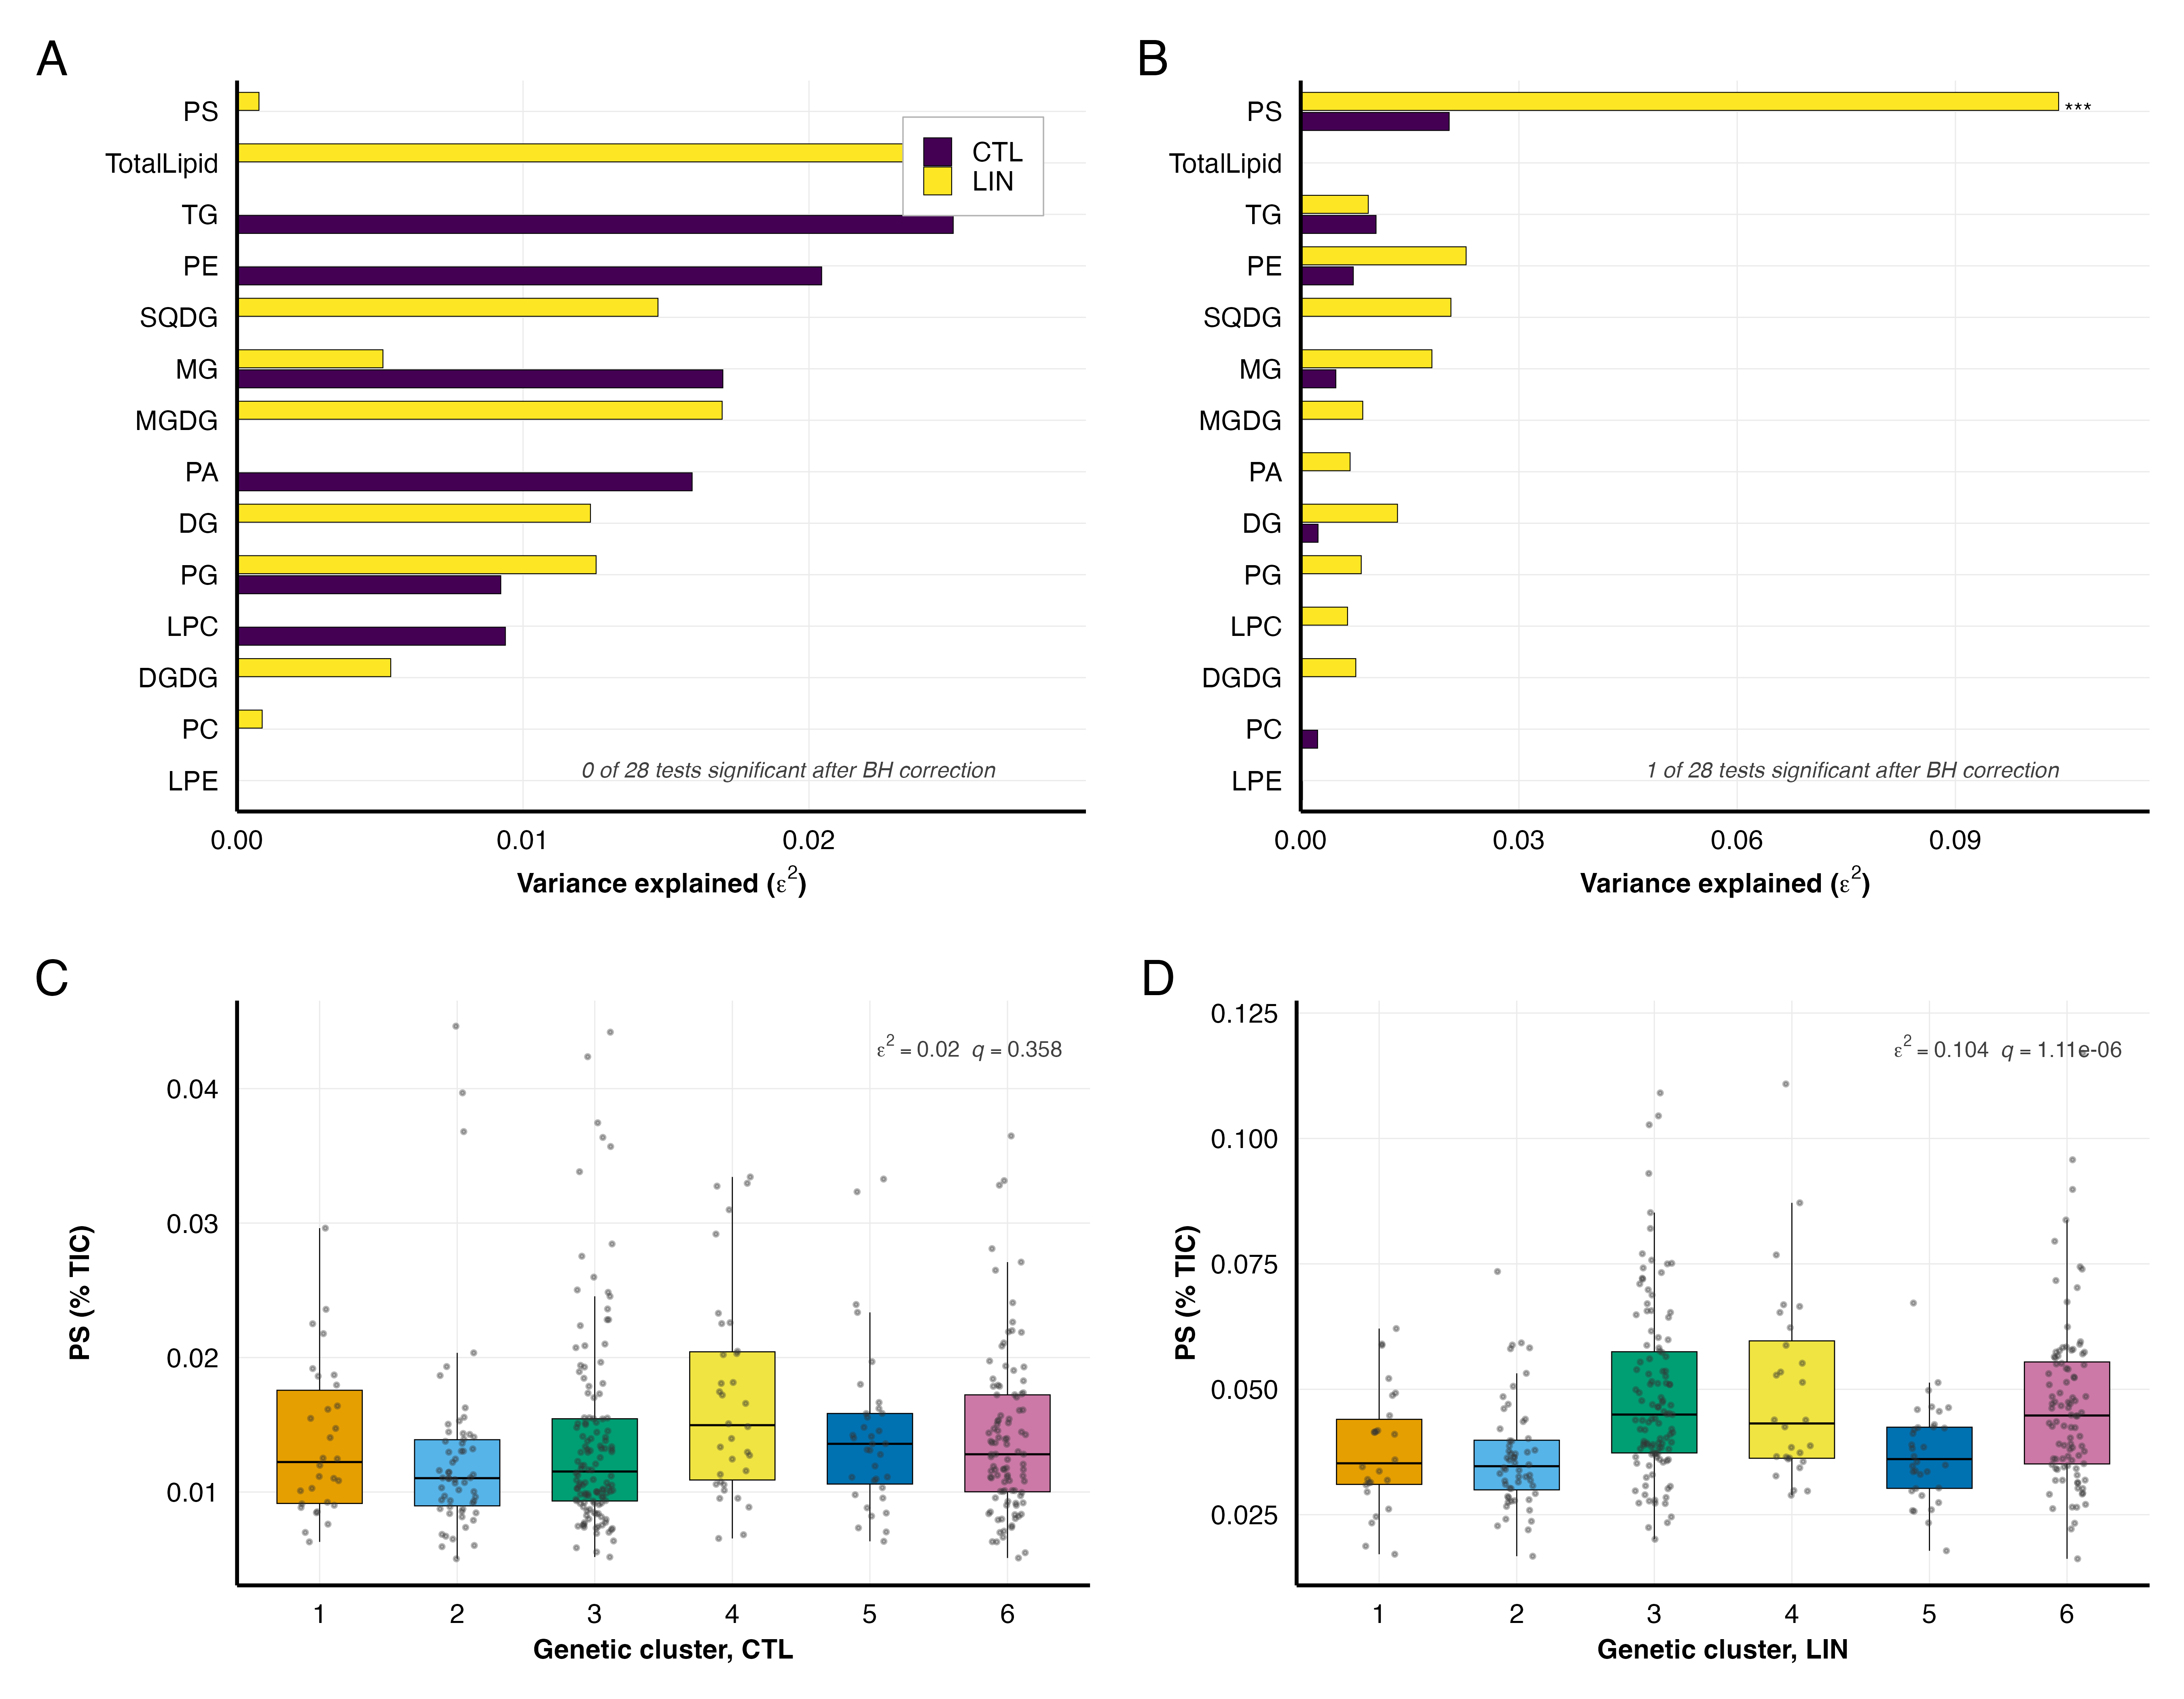
\includegraphics[width=0.95\textwidth]{fig/main/Figure1_Population_Structure.png}
\caption{\textbf{Lipid-class variation is largely independent of botanical race
and of population structure, except for PS.} \textbf{(A,B)}~Variance explained
($\varepsilon^2$) by botanical race (six groups) and by marker-based genetic
cluster ($K=6$), for total lipid signal and the 13 lipid classes, computed
within each field trial. Stars mark tests significant after Benjamini--Hochberg
correction. \textbf{(C,D)}~PS abundance (\% TIC) by genetic cluster in each
trial. Each panel keeps its own scale, since the comparison is between clusters
within a trial. PS under LIN is the only trait of the 28 tested that is
associated with cluster membership.}
\label{fig:fig1_population_structure}
\end{figure*}


\begin{table}[!ht]
\centering
\caption{\textbf{Genomic heritability of lipid-class sums, for the classes distinguishable from zero.}
Estimated by profile likelihood against the marker-based relationship matrix, using every accession of each
trial that is in the relationship matrix (389 under CTL, 357 under LIN) and every species of that class
detected in that trial. The phenotype is the summed spatially corrected intensity of the class on the
$\log_{10}$ scale, the same construction used for the per-species estimates above. Values are $h^2$ with
the 95\% profile-likelihood interval in brackets; $^{*}$ marks an interval excluding zero, the criterion
used throughout for calling a trait heritable. Four of the 17 classes meet it in one trial or the other.
All 17 are in Supplementary Table~S26. $N$ is the number of species summed into the class in that trial.}
\label{tab:classsum_h2}
\small
\begin{tabular}{lrlrl}
\toprule
 & \multicolumn{2}{c}{\textbf{CTL}} & \multicolumn{2}{c}{\textbf{LIN}} \\
\cmidrule(lr){2-3}\cmidrule(lr){4-5}
\textbf{Class} & \textbf{$N$} & \textbf{$h^2$} & \textbf{$N$} & \textbf{$h^2$} \\
\midrule
FA & 1 & 0.111 [0.000, 0.401] & 1 & 0.404 [0.153, 0.708]$^{*}$ \\
PS & 2 & 0.017 [0.000, 0.243] & 1 & 0.382 [0.167, 0.657]$^{*}$ \\
TG & 67 & 0.217 [0.000, 0.564] & 66 & 0.208 [0.017, 0.525]$^{*}$ \\
PA & 1 & 0.555 [0.252, 0.893]$^{*}$ & 2 & 0.000 [0.000, 0.123] \\
\bottomrule
\end{tabular}
\end{table}

\subsection*{Lipidome overview for CTL and LIN SAP}

We quantified a total of 266 lipid species, with 164 detected in both trials, 50 only in CTL, and 52 only in LIN, where ``trial-specific'' indicates detection above the threshold in one trial rather than absence in the other (Supplementary~\ref{fig:suppfig_s5_counts}). All the data are browsable in the SoLD Shiny application. TGs and PCs were the most diverse classes in both environments (TG: 67 in CTL, 66 in LIN; PC: 36 in CTL, 38 in LIN; Supplementary~\ref{fig:suppfig_s5_counts}). The species contributing most to between-genotype variance in each trial are listed in Supplementary Table~S4 (top-variance lipids).

Furthermore, we summarized lipid abundance as \%TIC (mean share of total annotated signal per sample), so values represent the relative signal in each condition. In both trials, the glycerolipids and glycerophospholipids dominated the annotated signal (CTL: 65.4\% and 30.3\%; LIN: 64.3\% and 30.7\%), while the prenol lipids were the only other category above 1\% (3.4\% and 4.2\%) (Fig.~\ref{fig:fig2_class_composition}A). The sterol lipids show the largest proportional change of any category, rising 5.1-fold from 0.04\% to 0.22\% of the annotated signal, almost all of it \textit{$\beta$}-sitosterol (0.039\% to 0.178\%). Both values are small, so the change cannot substantially alter the bulk composition.

Within the galactolipids and phospholipids, MGDG contributed the most with 32.7\% (CTL) and 30.1\% (LIN), while PC contributed 24.2\% and 23.3\%. DGDG (12.1\%, 12.2\%) and DG (13.0\%, 13.8\%) followed. TG increased from 2.6\% (CTL) to 4.9\% (LIN), while SQDG decreased from 2.8\% to 1.3\%. Overall, these lipids comprised 94.7\% (CTL) and 93.5\% (LIN) of annotated signals, with the remainder coming from sterols, terpenoids, prenols, fatty acids, and other minor categories (Fig.~\ref{fig:fig2_class_composition}B; Supplementary Table~S4, composition \%TIC). Because \%TIC values sum to 100, increases in one class reduce others. We therefore repeated the contrast on centered and additive log-ratio scales (CLR and ALR), which lack this constraint. Both gave the same ranking, with SQDG decreasing the most and PS increasing the most (Supplementary Table~S4, CLR and ALR contrasts). Furthermore, removing each botanical race group in turn or randomly deleting 20\% of accessions shifted the mean \%TIC of the largest class (PC) by at most 0.10 percentage points under CTL and 0.18 under LIN, with smaller changes for other classes (Supplementary Table~S3, composition stability). This implies that class shares were robust to panel composition.

Additionally, two minor pools show large changes masked in the bulk profile. PS increases from 0.014\% to 0.045\% of annotated signal, and its correlation with PC flips between trials ($r=0.43$ in CTL vs. $r=-0.34$ in LIN; Supplementary Table~S4, CLR correlation delta; Supplementary~\ref{fig:suppfig_s6_pcor}). Among lysophospholipids the two classes move in opposite directions. LPE rises from 0.006\% to 0.014\% of annotated signal while LPC falls on both log-ratio scales (CLR $-0.14$, ALR $-0.62$; Supplementary Table~S4, CLR and ALR contrasts), so the LPC/LPE ratio halves from 23.2 to 11.1. Both pools stay below 0.2\% in both trials.

After using PCA to assess how genotype and botanical race structure the diversity panel, we performed a similar analysis on the lipidomic data. Within each trial, PCA of major glycerolipid and glycerophospholipid pools showed that lipid class was the main driver of species-level variation (Supplementary~\ref{fig:suppfig_s7_pca}). Results for the remaining lipid classes are available in the Shiny app. TG species formed a distinct cluster separated from most membrane lipids in both CTL and LIN, though along different principal axes. Galactolipids and glycerophospholipids partly overlapped but occupied class-enriched regions, supporting class-level aggregation for downstream compositional and reaction-network analyses. 

\begin{figure*}[!ht]
\centering
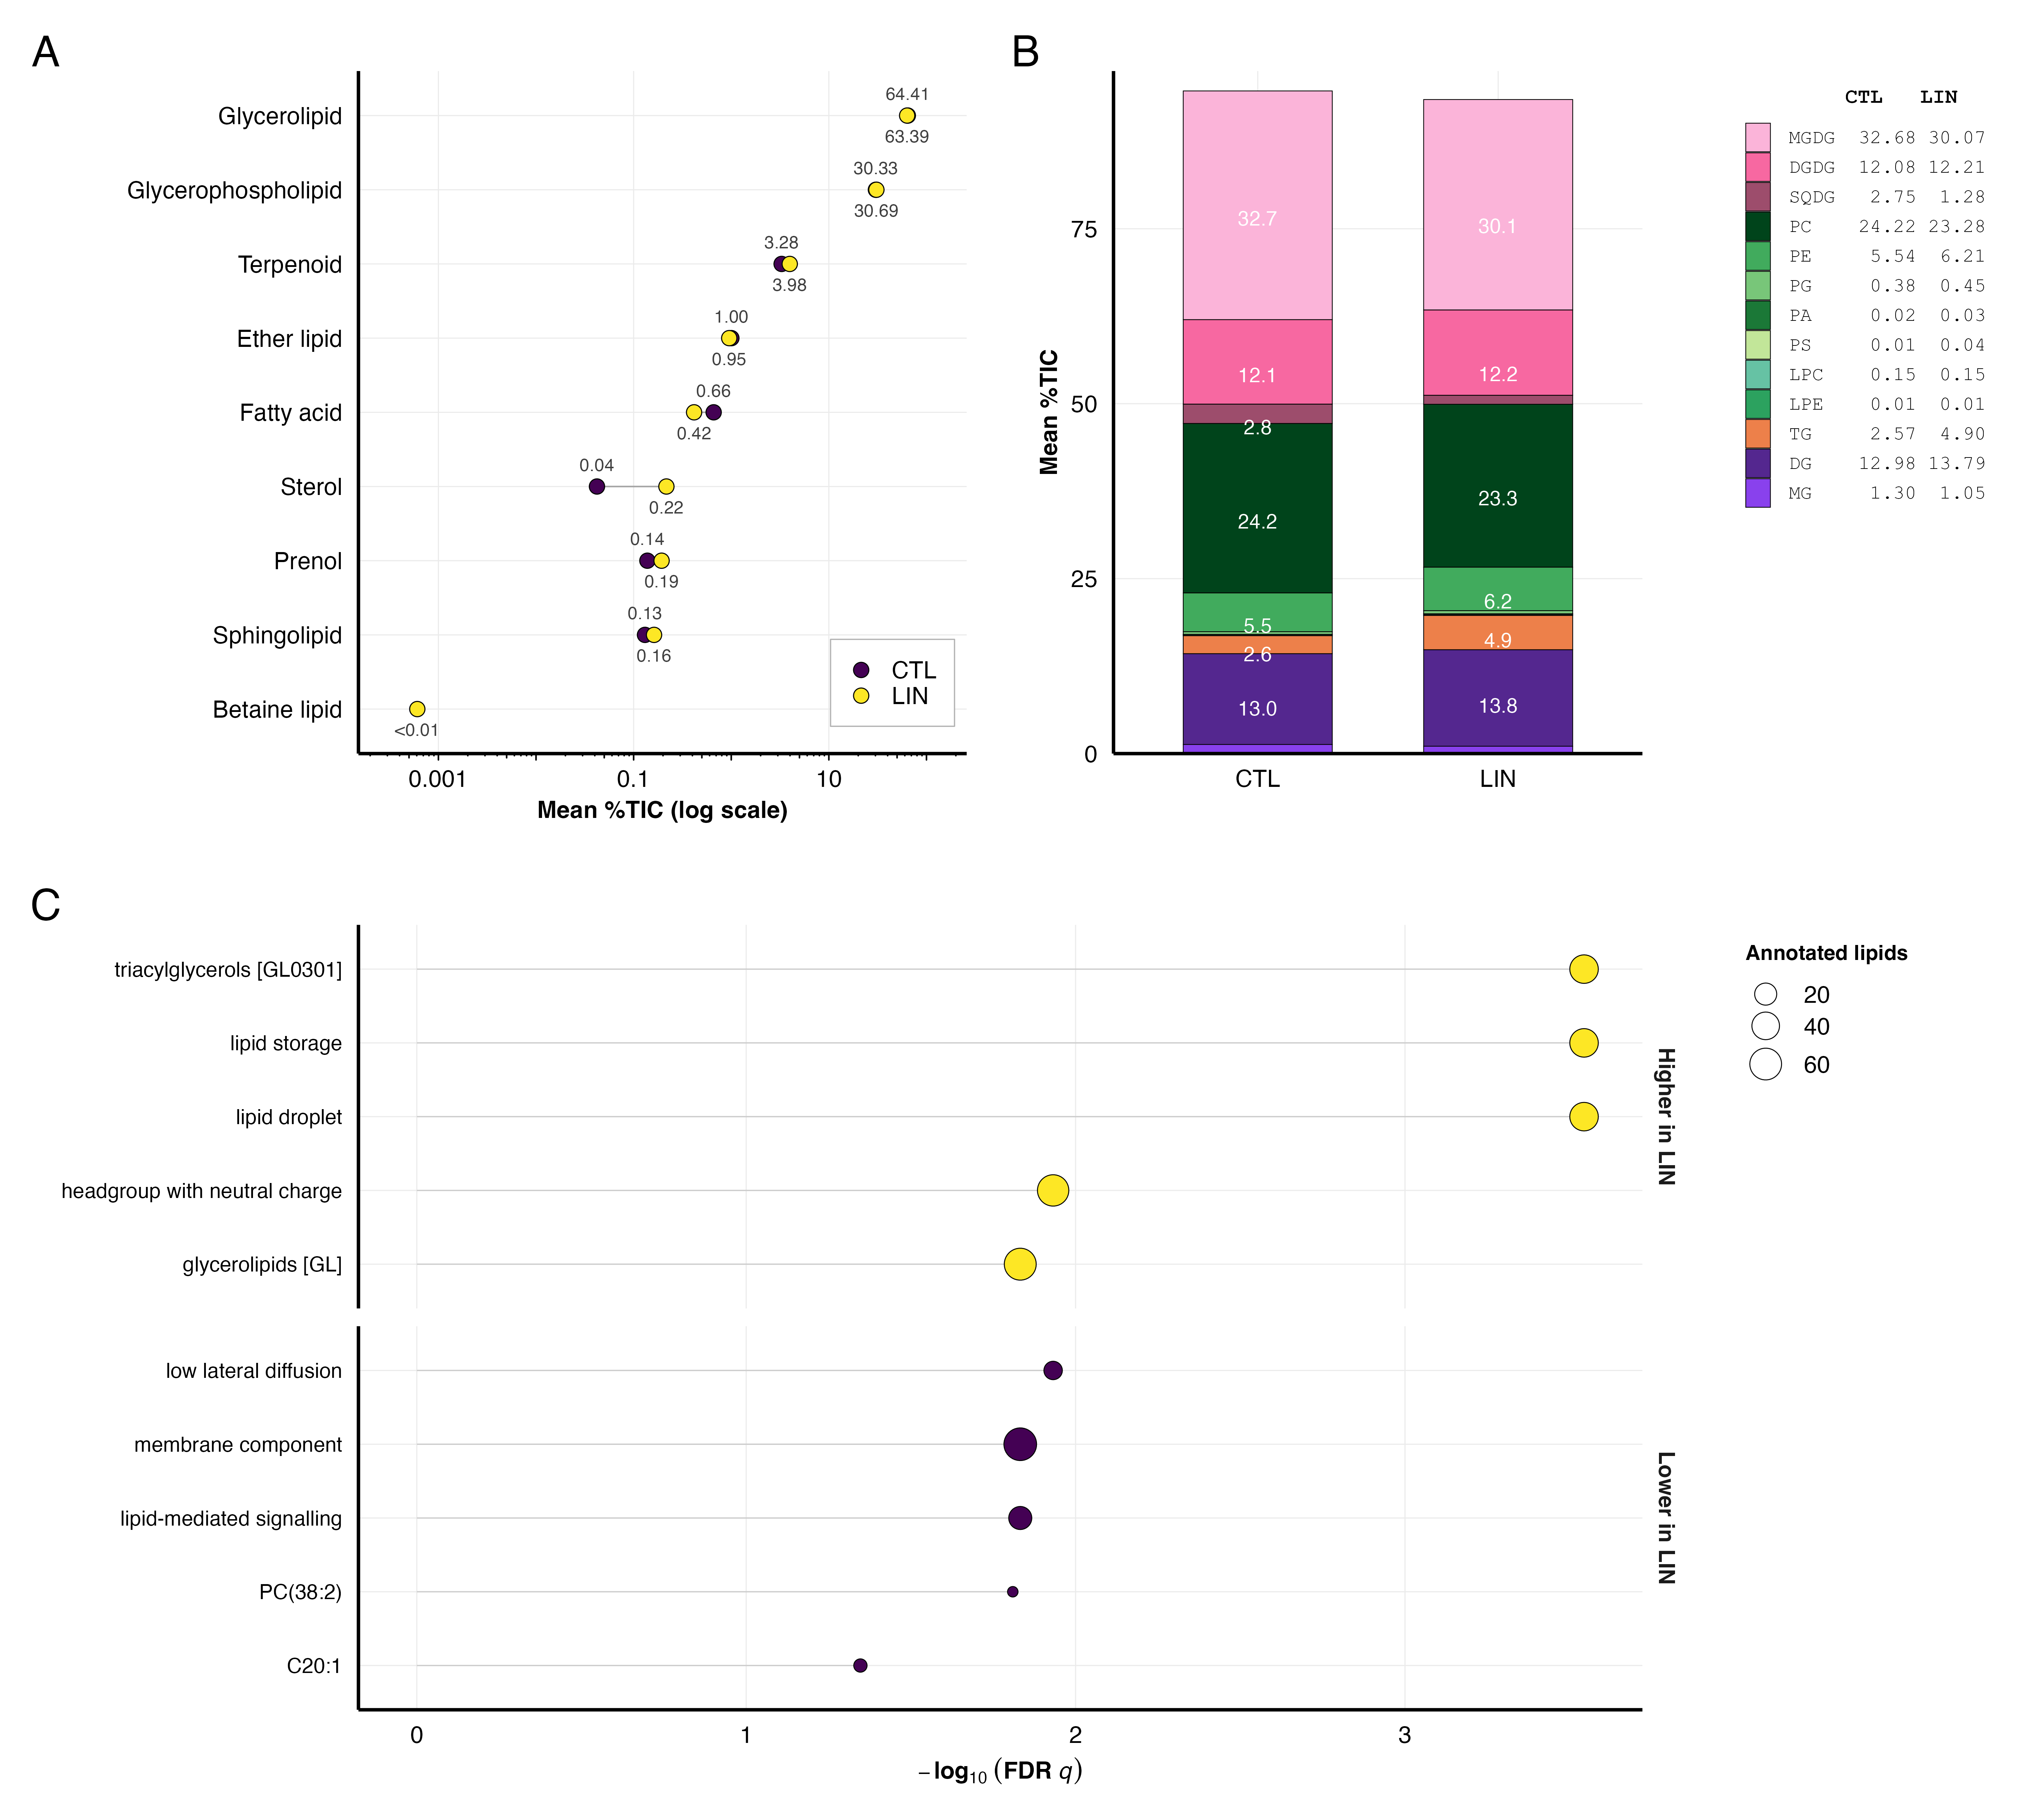
\includegraphics[width=\textwidth]{fig/main/Figure2_Class_Composition.png}
\caption{\textbf{Lipid-class composition of the SAP leaf lipidome in each field
trial.} Composition is \%TIC, the share of total annotated signal, taken per
sample and then averaged. \textbf{(A)}~Every annotated LIPID MAPS category on a log
scale, so categories below 1\% remain legible. \textbf{(B)}~The 13 focal lipid
classes, stacked; the bars stop between 93\% and 95\% because the remaining signal belongs
to the minor categories in (A). \textbf{(C)}~LION ontology terms significant at
FDR $q<0.05$, the ten strongest in each direction, sized by the number of
annotated lipids. Unlike (A) and (B), this panel is a direct CTL--LIN contrast,
and the two trials differ in year, field and acquisition batch.}
\label{fig:fig2_class_composition}
\end{figure*}

We next asked whether the class shifts were accompanied by shared structural and biophysical properties using LION, a lipid ontology that groups species into such categories \citep{Molenaar2019}. LION ranking analysis across the shared lipid species returned ten significant terms, five higher and five lower with respect to LIN (\(q<0.05\); Fig.~\ref{fig:fig2_class_composition}C; Supplementary Table~S5, LION enrichment). The higher LIN terms describe one pool of the 44 shared TG species plus 12 DG and 5 MG rising from 16.9\% to 19.7\%. The five higher terms in LIN all report the same result, that storage lipid increased, rising from 16.9\% to 19.7\% of annotated signal. The three lower terms in LIN are related to the membrane. \textit{Membrane component} is the bilayer itself, and it falls with the shared phospholipids, from 30.2\% to 28.5\% of annotated signal, almost all of it PC (24.2\% to 21.9\%). \textit{Low lateral diffusion} is the tightly packed, ordered fraction of that bilayer, and \textit{lipid-mediated signaLINg} is the DG, PA, and lyso pool released by membrane turnover, and both are lower in LIN as well. Together, these terms suggest a leaf holding less bilayer and more storage lipid under LIN, consistent with acyl chains being routed into droplets rather than into new membrane.

Finally, to describe class chemistry beyond abundance, we summarized each lipid class in a reduced chemical space using the abundance-weighted mean total carbon number and double-bond count across molecular species (Supplementary~\ref{fig:suppfig_s8_chem}; Supplementary Table~S5, chemical space). Carbon number cleanly separates the lipid. Lysophospholipids and monoacylglycerols have 16–18 carbons, diacyl lipids have 33–37, and TG has 51.0 (CTL) and 54.6 (LIN). Diacyl unsaturation varies independently of chain length, increasing from PG (0.6 double bonds) to PC (2.1) to MGDG (5.7). Across trials, PE shows the largest unsaturation increase (2.7 to 3.4 double bonds) among classes with >10 species. Otherwise, aside from a higher TG carbon number, all classes except PS change by <1 carbon and <0.25 double bonds. PS is not comparable (two species to one). Thus, within-class chemistry is largely stable, and CTL–LIN differences mainly reflect shifts in class proportions, not chain composition.

Compared with CTL, four population-wide shifts characterize the LIN lipidome: (i) SQDG depletion, (ii) TG enrichment, (iii) a phospholipid rebalancing centered on PS, and (iv) an LPC/LPE balance shifted toward LPE. All four shifts rest on the abundance and composition analyzes. LION corroborates only the TG shift, with its remaining terms tracking the same glycerolipid-versus-membrane contrast. Because the trials also differ by year, field, planting date, and analytical batch, these shifts characterize LIN as a whole and cannot be attributed solely to nutrient supply, cold, and chemicals. The reaction-network and GWAS sections that follow ask which reactions and loci accompany these changes.

\subsection*{GWAS recovers more genomic regions under LIN and more trait-sharing per region under CTL}

We ran separate GWAS for each individual lipid trait, lipid-class sum, and lipid-class ratio in both trials (747 in total: 220 individual species and 153 class sums and ratios under CTL, 221 and 153 under LIN), using a univariate linear mixed model with the first three genotype PCs to account for population structure (Fig.~\ref{fig:gwas_manhattan}). SNPs surpassing the Bonferroni genome-wide significance threshold ($p \leq 8.19 \times 10^{-9}$ for CTL and $8.22 \times 10^{-9}$ for LIN) were mapped to candidate genes using the LD-based cutoff of 0.4. Under CTL, this identified 1,062 candidate genes for individual lipids and 54 for class sums and ratios (Supplementary Table~S6). Under LIN, the same procedure identified 4,370 and 385 candidate genes (Supplementary Table~S6). Manhattan and QQ plots for every lipid phenotype in both trials are available in the SoLD Shiny application.

Candidate gene counts do not equal signal counts because one significant SNP tags all genes in its LD window. After binning candidates into 250 kb windows, there were 358 distinct windows under CTL and 949 under LIN. So, LIN captures $\sim$2.6$\times$ more loci, not the four-fold suggested by gene counts. Hence, CTL loci average 3.0 candidate genes, while LIN loci average 4.6. Candidates also differ in phenotype recurrence. Under CTL, 586 of 1,062 individual-lipid candidates were linked to more than one phenotype (median 2, maximum 13), compared to 1,474 of 4,370 under LIN (median 1, maximum 8). Thus, in the individual-lipid layer, CTL yields fewer loci with many lipid associations, while LIN yields more loci with few. The class-sum and ratio layer is too small under CTL for the same contrast, with 27 of its 54 candidates linked to more than one phenotype (median 1.5, maximum 6) compared to 84 of 385 under LIN (median 1, maximum 13). Because lipid phenotypes are inherently highly correlated by design, these recurrence counts serve as descriptive summaries rather than formal tests against a null hypothesis, while the cross-trial comparison presented in the next section is evaluated explicitly.

In the CTL individual-lipid layer, the strongest association and the most recurrent locus was \texttt{SORBI\_3001G258000} (protein kinase domain-containing protein; 6 phenotypes; $p = 3.17\times10^{-9}$; $r^2_{\max}=0.66$), one of nine genes in a chromosome 1 interval annotated by an F-box protein in Table \ref{tab:top_loci}. In the CTL sum/ratio layer, the strongest association was \texttt{SORBI\_3006G010000} (FCP1 homology domain-containing protein; $p = 2.02\times10^{-10}$; $r^2_{\max}=0.67$), and the most recurrent locus was \texttt{SORBI\_3001G258000} (protein kinase domain-containing protein; 6 phenotypes; $p = 3.17\times10^{-9}$; $r^2_{\max}=0.66$) (Table~\ref{tab:top_loci}). In the LIN individual-lipid layer, the strongest association was observed for \texttt{SORBI\_3008G081000}, an uncharacterized protein ($p = 4.50\times10^{-33}$; $r^2_{\max}=0.94$), and the most recurrent locus was \texttt{SORBI\_3010G150600} (8 phenotypes; $p = 1.41\times10^{-18}$; $r^2_{\max}=1.0$), one of nine genes in a chromosome~10 interval labelled by a peroxidase. In the LIN sum/ratio layer, the strongest association and the most recurrent locus were both \texttt{SORBI\_3004G004800} (soluble acid invertase; 13 phenotypes; $p = 7.07\times10^{-16}$; $r^2_{\max}=0.69$) (Table~\ref{tab:top_loci}). The full candidate-gene lists are browsable in the SoLD Shiny application. Thus, more heritable traits are  easier to map, so the larger LIN candidate list follows from the heritability result.

\begin{table*}[!ht]
\centering
\caption{\textbf{The most recurrent GWAS loci under CTL and LIN.} The five loci associated with the largest number of phenotypes in each trial and trait layer. A locus is one signal, defined as all candidate genes sharing a trial, trait layer, chromosome and best $p$-value, so the genes tagged by one lead SNP occupy a single row. Interval, the span of the tagged genes in Mb; Genes, the number of candidate genes the signal tags; Gene, the first gene in that interval carrying a functional annotation, given as a label for the locus rather than as a causal assignment; Traits, the number of lipid phenotypes associated with the locus. Recurrence counts are descriptive summaries of the candidate tables and not a test against a null expectation, since lipid phenotypes are correlated by construction.}
\label{tab:top_loci}
\scriptsize
\begin{tabular}{llrllrl}
\toprule
\textbf{Trait layer} & \textbf{Interval (Mb)} & \textbf{Genes} & \textbf{Gene} & \textbf{Putative function} & \textbf{Traits} & \textbf{$P$} \\
\midrule
\multicolumn{7}{l}{\textbf{CTL}} \\
Individual lipids & 5:61.66--61.75 & 2 & \texttt{SORBI\_3005G148500} & FBD domain-containing protein & 13 & $1.55\times10^{-16}$ \\
 & 10:32.68--32.68 & 1 & \texttt{SORBI\_3010G140800} & Uncharacterized protein & 13 & $1.24\times10^{-14}$ \\
 & 5:24.10--24.13 & 2 & \texttt{SORBI\_3005G110120} & Uncharacterized protein & 12 & $8.19\times10^{-15}$ \\
 & 1:60.64--60.65 & 2 & \texttt{SORBI\_3001G318000} & Glutathione transferase & 11 & $3.05\times10^{-16}$ \\
 & 6:35.88--36.24 & 3 & \texttt{SORBI\_3006G049600} & Methyltransferase type~11 domain-containing protein & 11 & $1.18\times10^{-14}$ \\
\addlinespace
Sums / ratios & 1:30.37--30.84 & 9 & \texttt{SORBI\_3001G257300} & F-box domain-containing protein & 6 & $3.17\times10^{-9}$ \\
 & 6:1.45--1.57 & 6 & \texttt{SORBI\_3006G010000} & FCP1 homology domain-containing protein & 3 & $2.02\times10^{-10}$ \\
 & 1:30.70--31.02 & 5 & \texttt{SORBI\_3001G258500} & GDSL esterase/lipase & 3 & $5.80\times10^{-9}$ \\
 & 5:1.12--1.52 & 13 & \texttt{SORBI\_3005G012200} & Serine/threonine protein kinase & 2 & $9.63\times10^{-10}$ \\
 & 1:50.79--50.89 & 4 & \texttt{SORBI\_3001G266600} & Plant lipid transfer protein & 2 & $5.42\times10^{-9}$ \\
\midrule
\multicolumn{7}{l}{\textbf{LIN}} \\
Individual lipids & 10:43.19--43.39 & 9 & \texttt{SORBI\_3010G149700} & Peroxidase & 8 & $1.41\times10^{-18}$ \\
 & 10:43.62--43.63 & 2 & \texttt{SORBI\_3010G151000} & CMP-sialic acid transporter~1 & 8 & $5.94\times10^{-12}$ \\
 & 2:14.37--14.49 & 12 & \texttt{SORBI\_3002G116200} & Adenylate kinase isoenzyme~6 homolog & 7 & $3.76\times10^{-13}$ \\
 & 1:16.45--16.68 & 3 & \texttt{SORBI\_3001G187300} & Molybdate transporter~1 & 7 & $1.16\times10^{-11}$ \\
 & 10:50.10--50.18 & 4 & \texttt{SORBI\_3010G170000} & O-acyltransferase (\textit{DGAT1}) & 6 & $3.16\times10^{-15}$ \\
\addlinespace
Sums / ratios & 4:0.42--0.78 & 27 & \texttt{SORBI\_3004G004800} & Soluble acid invertase & 13 & $7.07\times10^{-16}$ \\
 & 3:7.54--7.78 & 15 & \texttt{SORBI\_3003G087100} & Protein MAO HUZI 4, chloroplastic & 10 & $1.41\times10^{-15}$ \\
 & 3:7.48--7.48 & 1 & \texttt{SORBI\_3003G086600} & LOB domain-containing protein & 10 & $3.62\times10^{-15}$ \\
 & 4:0.18--0.43 & 3 & \texttt{SORBI\_3004G002350} & Small nuclear ribonucleoprotein Sm~D3 & 10 & $1.48\times10^{-14}$ \\
 & 3:71.32--71.66 & 8 & \texttt{SORBI\_3003G406600} & SBP-type domain-containing protein & 9 & $9.97\times10^{-15}$ \\
\bottomrule
\end{tabular}
\end{table*}

\begin{figure*}[!t]
\centering
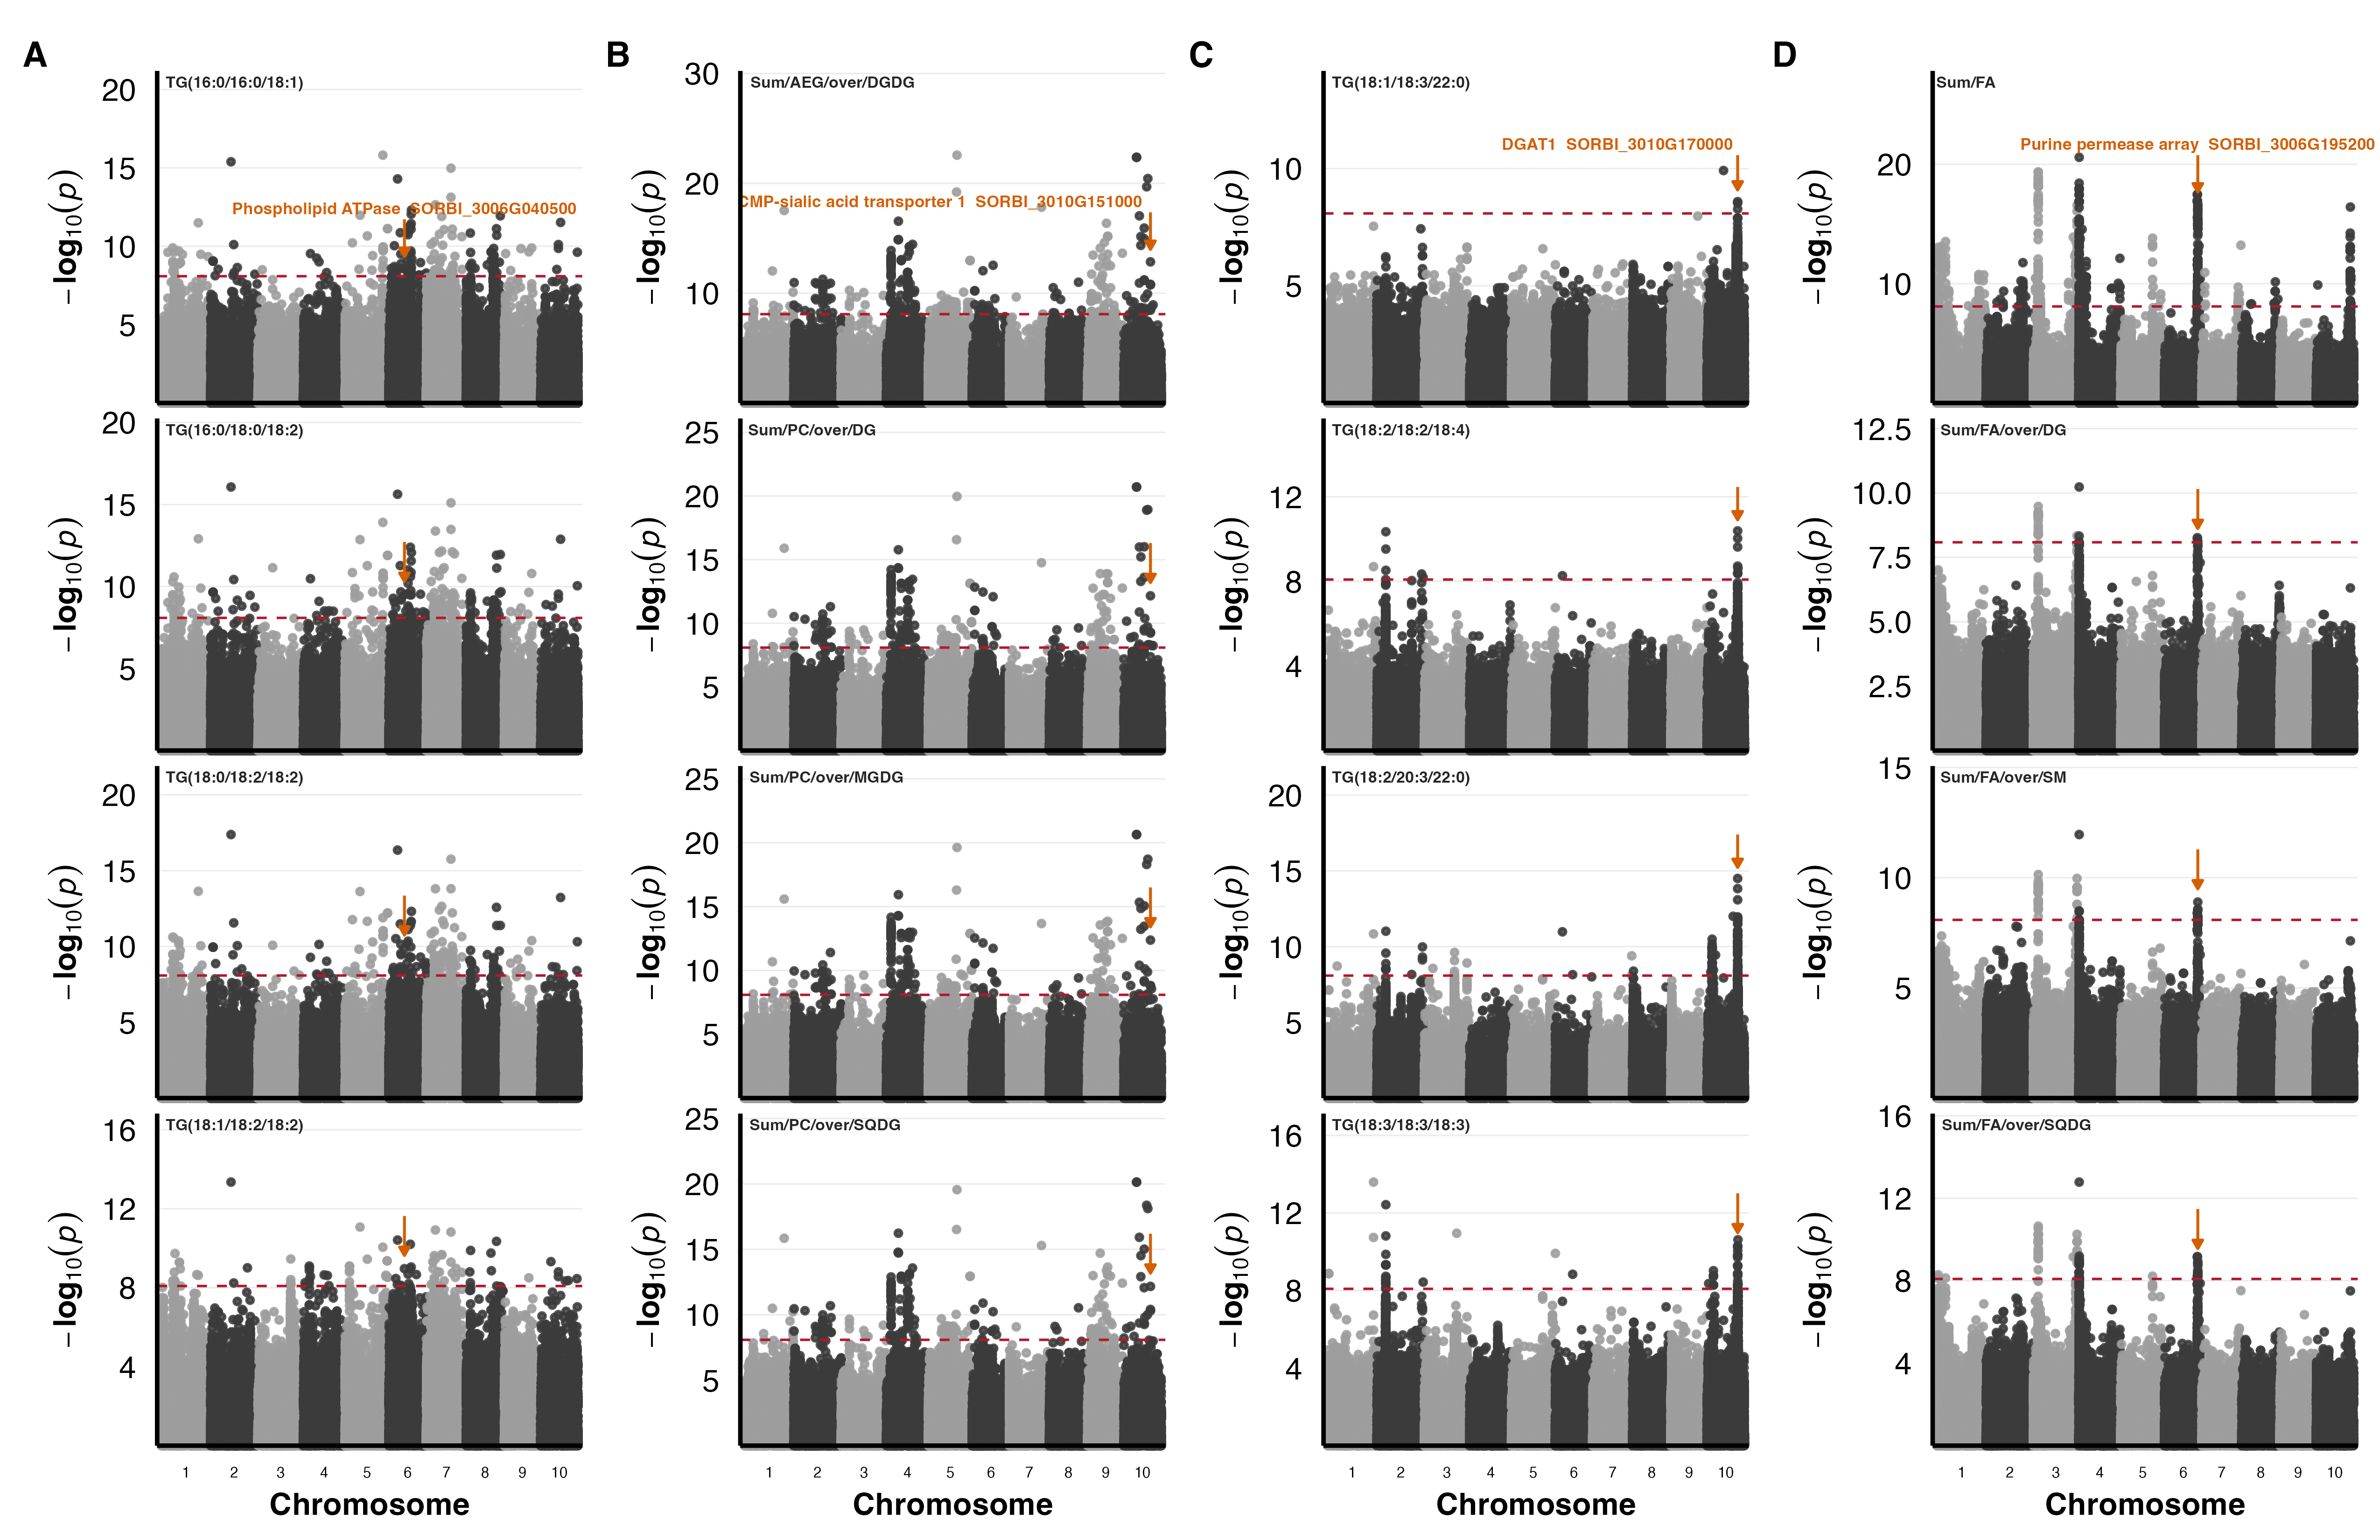
\includegraphics[width=\textwidth]{fig/main/Figure3_GWAS_Manhattan.png}
\caption{\textbf{The same candidate locus recurs across multiple lipid phenotypes
within each trial.} Each column stacks four phenotypes that share one candidate
locus. An orange arrow marks the lead SNP for that locus in every plot, and the
candidate gene is named once, above the arrow in the top plot of the column.
\textbf{(A)}~CTL individual lipids, sharing \texttt{SORBI\_3006G040500}
(phospholipid-transporting ATPase, chromosome~6). \textbf{(B)}~CTL class sums and
ratios, sharing \texttt{SORBI\_3010G151000} (CMP-sialic acid transporter~1,
chromosome~10). \textbf{(C)}~LIN individual lipids, sharing
\texttt{SORBI\_3010G170000} (\textit{DGAT1}, chromosome~10). \textbf{(D)}~LIN
class sums and ratios, sharing the chromosome~6 purine-permease array
(\texttt{SORBI\_3006G195200}). Within a column, each plot is identified by the
trait named in its upper-left corner. Red dashed horizontal lines mark the
Bonferroni genome-wide threshold ($p \leq 8.19 \times 10^{-9}$). Point shading
alternates by chromosome. All Manhattan and QQ plots for the full phenotype set
are browsable in the SoLD Shiny application.}
\label{fig:gwas_manhattan}
\end{figure*}

\begin{figure*}[!ht]
\centering
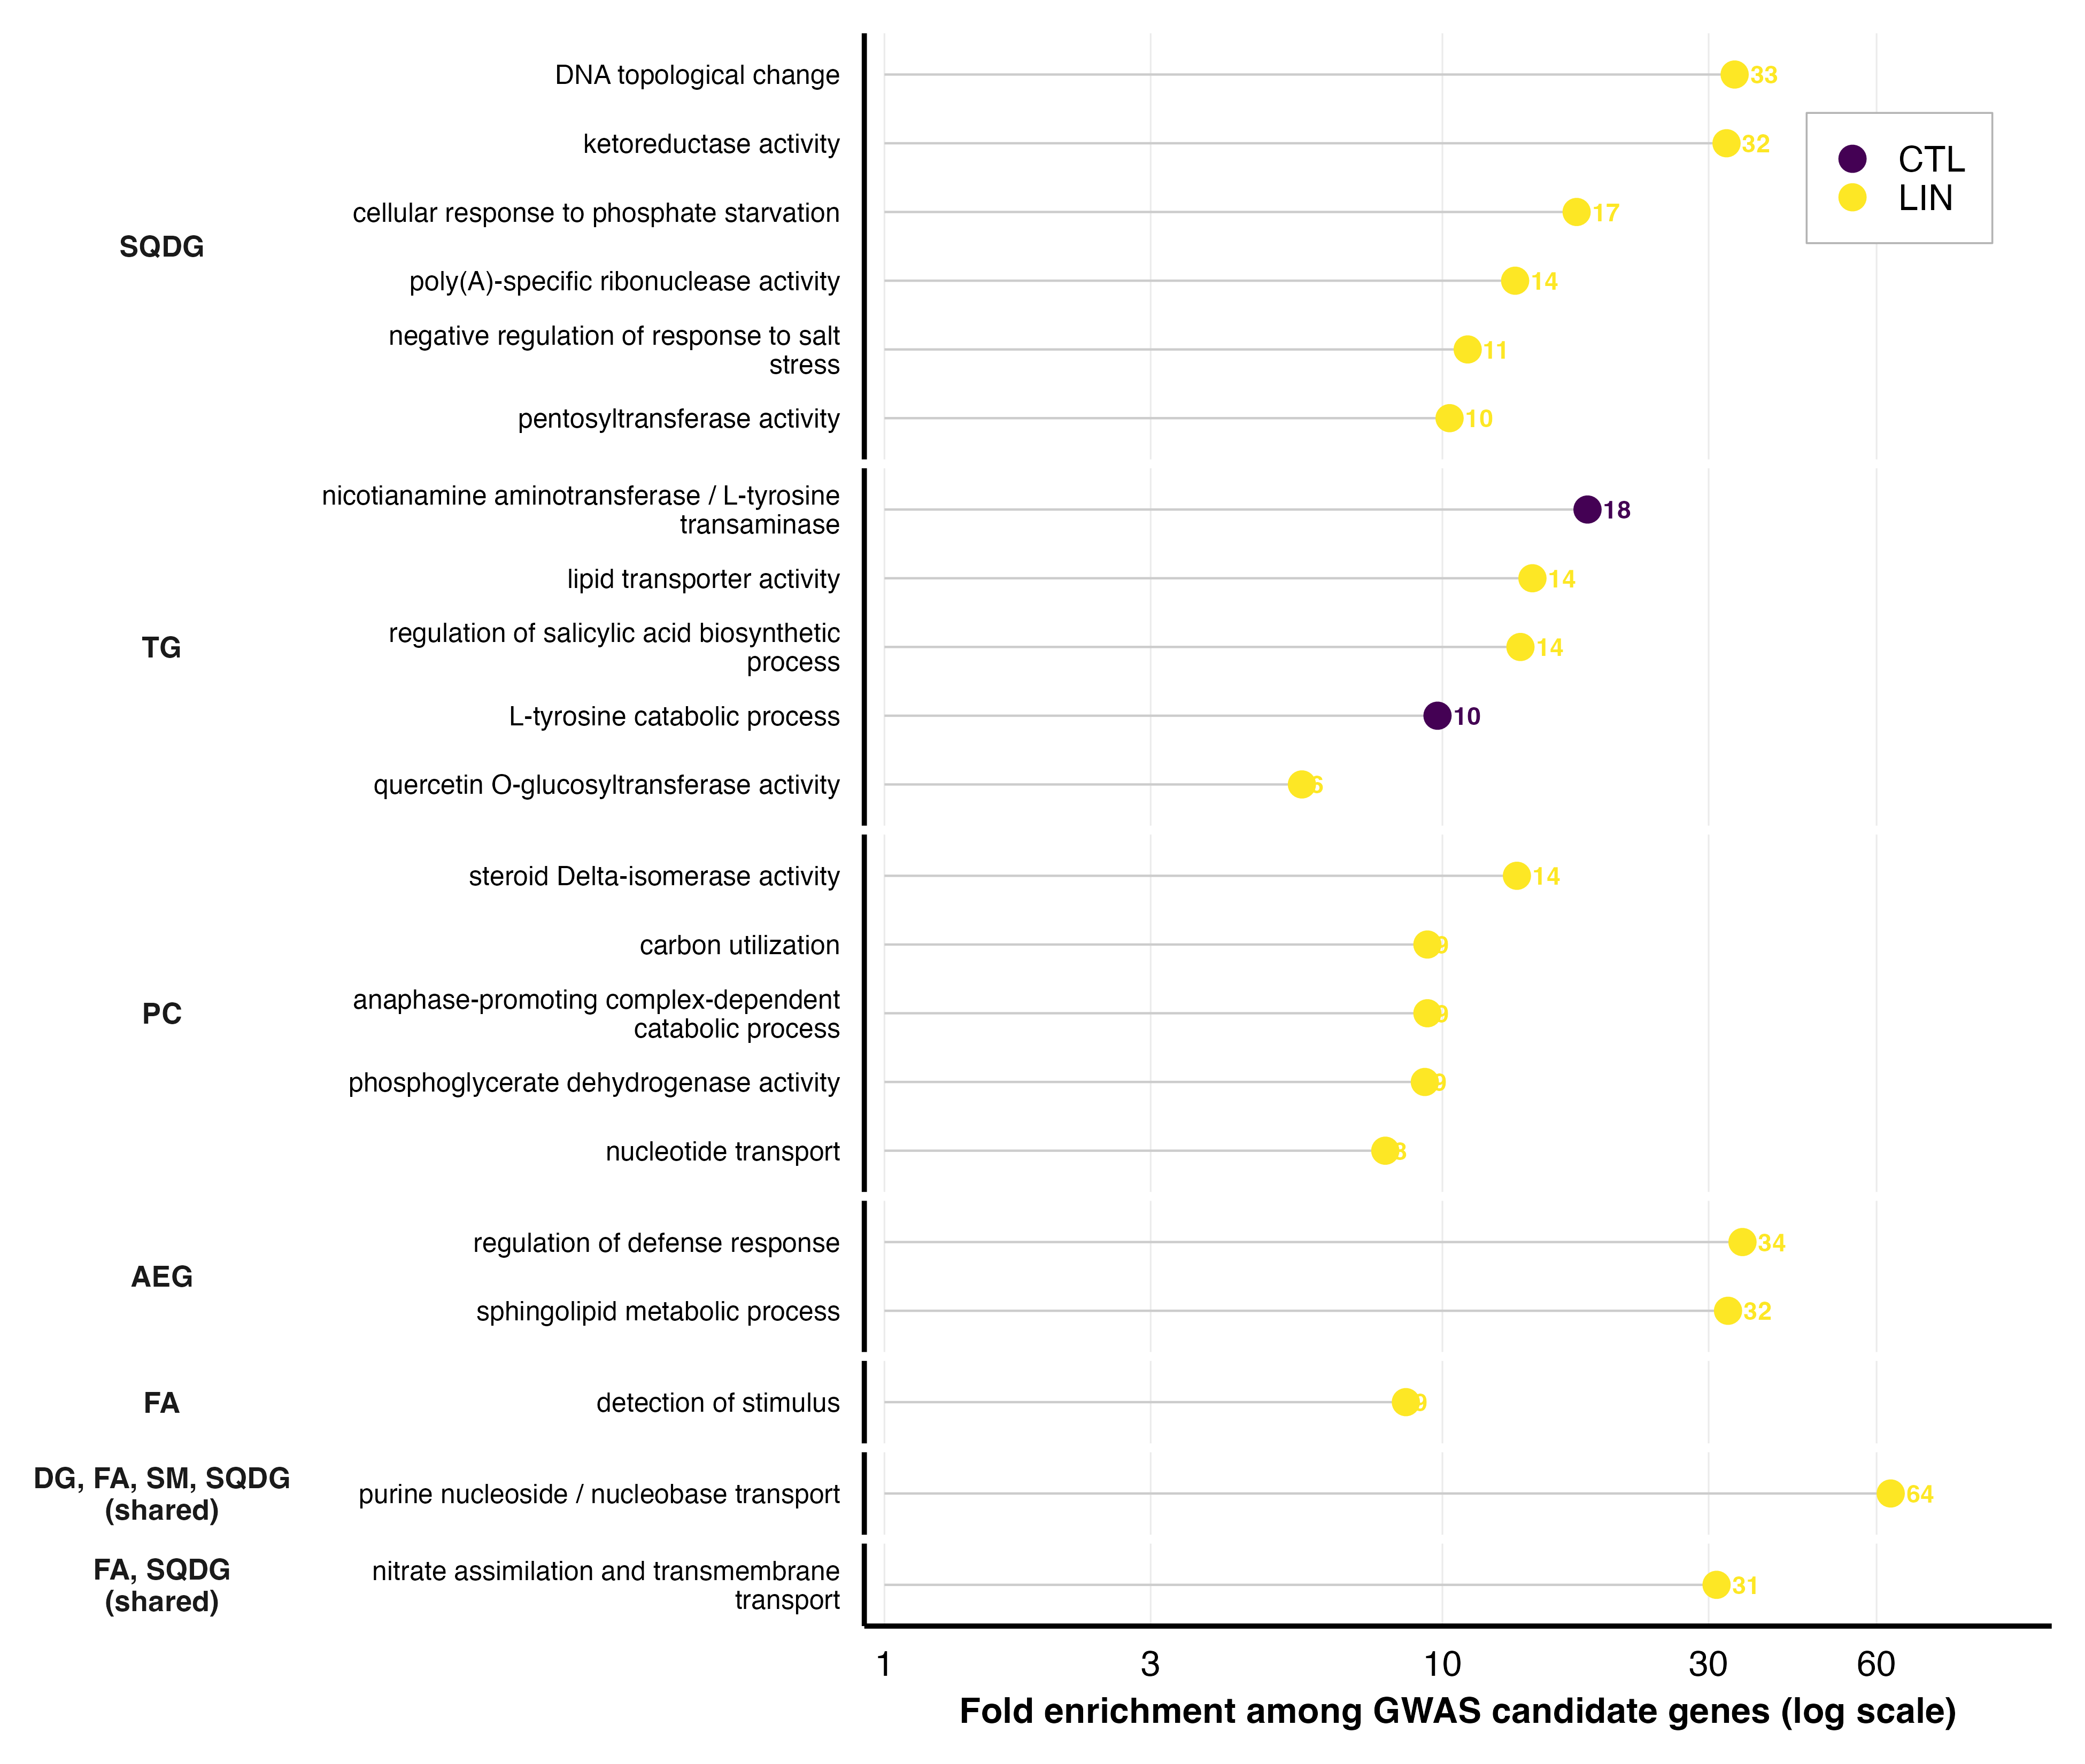
\includegraphics[width=\textwidth]{fig/main/Figure5_GO_BP_LDaware.png}
\caption[GO terms enriched among GWAS candidate genes, by lipid class]{\textbf{Gene
Ontology terms enriched among LD-mapped GWAS candidate genes, grouped by the lipid
class whose traits produced them.} Twenty-three gene sets are shown. Each began as an
enrichment passing the LD-aware permutation null ($q_{\mathrm{LD}}<0.05$); terms
sharing an identical candidate-gene set were then merged, first within a stratum,
where the Gene Ontology's nested parent and child terms describe one locus several
times, and then across lipid class, trait layer and ontology, where class sums and
ratios share candidate genes by construction. Of the 285 gene sets remaining
after those merges, the figure shows the strongest four per lipid class among those
that draw on at most 30 background genes and span at least two independent
intervals. The background limit is a criterion of interpretability rather than of
significance: terms such as \textit{zinc ion binding} (909 background genes) or
\textit{transmembrane transport} (865) pass the permutation null without naming a
lipid-related process. The interval requirement removes 17 gene sets that reach
high fold enrichment from a single LD block. Each label carries the number of
independent intervals supporting it, and every tested term is in Supplementary
Tables S16--S18.
Points give fold enrichment over chance on a logarithmic axis and are coloured by
trial. Left-hand strips name the lipid class; the two strips marked shared are gene
sets recurring across several classes, which are correspondingly less specific. The
complete set of 285 gene sets, with the number of independent 250\,kb intervals
supporting each, is given in Supplementary Table~S16 (loci collapsed).}
\label{fig:go_bp_main}
\end{figure*}

\subsection*{LD-aware GO enrichment reduces the candidate lists to a small number of interpretable terms}

Both candidate lists were too large to inspect gene by gene, so we tested Gene Ontology (GO) biological-process and molecular-function terms for over-representation within each lipid class and trial, using a permutation null that preserves LD-block structure. This distinguishes terms supported by multiple independent intervals from those driven by a single LD block.

In total, 344 of 1{,}292 tested terms passed the LD-aware null ($q_{\mathrm{LD}}<0.05$). Because GO terms are nested and class sums and ratios share candidate genes, we merged terms with identical gene sets, leaving 217 term gene-set combinations across 159 distinct terms (Supplementary Table~S16, loci collapsed). Of these, 87 draw on $\leq 30$ background genes, while the rest were too broad to interpret (\textit{zinc ion binding}, 909 genes; \textit{transmembrane transport}, 865). Seventy-one of the 87 are supported by two or more independent intervals, and the remaining 16 rest on a single LD block. Figure~\ref{fig:go_bp_main} shows the strongest four per lipid class among the 71, giving 22 gene sets.

Those 22 gene sets are unevenly split between trials, with 18 under LIN and 4 under CTL, the same asymmetry that the candidate counts show. All four CTL gene sets come from TG traits. The LIN gene sets primarily focus on nutrient transport and signaling. \textit{Cellular response to phosphate starvation} is the strongest of them, at $51\times$ enrichment across three independent intervals. \textit{Nitrate transmembrane transporter activity} follows from fatty-acid traits at $25\times$ across two intervals, and \textit{sphingolipid metabolic process} from AEG at $35\times$. Fatty acids, PC, and TG each contribute four gene sets, and SQDG three. Enrichment therefore narrows five thousand candidate genes to a short list that could be used for functional validation.

\subsection*{Candidate genes overlap between trials only for individual species, and the overlap does not survive collapsing linkage}

The two trials recovered largely different candidate lists, but different GO terms cannot indicate whether the underlying genetics differ. We therefore counted how many candidate genes the two conditions share and compared that count with the chance expectation from the 34{,}027 \textit{Sorghum bicolor} v3.1 gene models, both at gene resolution and after collapsing linked genes into 100, 250, and 500 kb windows (Fig.~\ref{fig:fig7_ctl_lin_overlap}). Overlap was tested with a hypergeometric test and summarized as fold enrichment over chance and as the Jaccard index, the proportion of all candidate genes appearing in both conditions.

At the gene level, the two candidate sets overlapped more than chance, with 291 genes shared against 140 expected ($2.07\times$, $p = 1.2\times10^{-35}$), but the excess comes entirely from the individual-lipid layer ($2.07\times$, $p = 2.7\times10^{-34}$; Table~\ref{tab:overlap}; Supplementary Table~S20). The class-sum and ratio layer shares no genes at all between trials, against 0.6 expected by chance, so it is neither enriched nor depleted, only empty. The shared genes are, in any case, a small fraction of the total, with a Jaccard index of 0.056. Within the individual-lipid layer, the excess is carried by TG and PC ($1.74\times$ and $3.47\times$, $q<0.02$), while fatty acids overlap no more than chance and four further classes share no genes at all, including SQDG despite its 400 LIN candidates (Table~\ref{tab:overlap_class}).

This mainly reflects LD, because each association maps every gene in its window, and gene-dense regions are mapped repeatedly in both trials. Because no window size is objectively correct for collapsing linkage, we repeated the test at 100, 250, and 500 kb and read the trend across them as the result. For individual lipids, the excess fell at every step, from $2.07\times$ at gene level to $1.17\times$ at 100 kb and $1.05\times$ at 250 kb, where it was no longer significant ($p = 0.22$), so loci recovered in the two trials are no more concordant than two independent samples of the same genome. The class-sum and ratio layer share no window at any of the three sizes. Moreover, recovering the same gene never meant recovering it for the same lipid. Of the 291 shared genes, none are candidates for the same trait in both trials, although 13 traits have significant associations in both. Candidate gene counts are inflated several-fold by LD in both layers.

\begin{table*}[!ht]
\centering
\caption{\textbf{Cross-trial overlap of GWAS candidates at gene and locus resolution.} Overlap between CTL and LIN candidate sets, tested against a background of 34{,}027 annotated gene models (gene level) or of all genome windows containing at least one gene (locus level). Fold, observed/expected shared; $J$, Jaccard index; $P$, hypergeometric (right-tail) test. Bold rows are the resolutions at which LD blocks are effectively collapsed.}
\label{tab:overlap}
\scriptsize
\begin{tabular}{llrrrrrrl}
\toprule
\textbf{Resolution} & \textbf{Trait layer} & \textbf{CTL} & \textbf{LIN} & \textbf{Shared} & \textbf{Exp.} & \textbf{Fold} & \textbf{$J$} & \textbf{$P$} \\
\midrule
Gene   & All layers          & 1091 & 4376 & 291 & 140.3 & 2.07 & 0.056 & $1.2\times10^{-35}$ \\
Gene   & Individual lipids   & 1062 & 4370 & 282 & 136.4 & 2.07 & 0.055 & $2.7\times10^{-34}$ \\
Gene   & Class sums / ratios &   54 &  385 &   0 &   0.6 & --- & 0.000 & 1 (n.s.) \\
\midrule
100 kb & Individual lipids   &  494 & 1556 & 185 & 158.7 & 1.17 & 0.099 & $4.7\times10^{-3}$ \\
100 kb & Class sums / ratios &   23 &  118 &   0 &   0.6 & --- & 0.000 & 1 (n.s.) \\
\textbf{250 kb} & \textbf{Individual lipids} & 351 & 948 & 153 & 146.0 & \textbf{1.05} & 0.133 & \textbf{0.22} \\
250 kb & Class sums / ratios &   17 &   72 &   0 &   0.5 & --- & 0.000 & 1 (n.s.) \\
\textbf{500 kb} & \textbf{Individual lipids} & 275 & 634 & 146 & 140.7 & \textbf{1.04} & 0.191 & \textbf{0.26} \\
500 kb & Class sums / ratios &   13 &   50 &   0 &   0.5 & --- & 0.000 & 1 (n.s.) \\
\bottomrule
\end{tabular}
\end{table*}

\begin{table}[!ht]
\centering
\caption{\textbf{Per-class cross-trial overlap of individual-lipid GWAS candidates.} Genes were assigned to a lipid class through the phenotypes with which they were associated. $q$, Benjamini--Hochberg-adjusted hypergeometric $P$-value. n.s., not significant.}
\label{tab:overlap_class}
\small
\begin{tabular}{lrrrrl}
\toprule
\textbf{Class} & \textbf{CTL} & \textbf{LIN} & \textbf{Shared} & \textbf{Fold} & \textbf{$q$} \\
\midrule
TG          & 832 &  892 & 38 & 1.74 & $5.3\times10^{-3}$ \\
PC          &  52 & 1319 &  7 & 3.47 & $1.3\times10^{-2}$ \\
Fatty acid  & 105 & 2417 &  6 & 0.80 & 1 (n.s.) \\
Terpenoid   &  45 &   49 &  0 & ---  & 1 (n.s.) \\
DG          &  11 &   31 &  0 & ---  & 1 (n.s.) \\
SQDG        &   8 &  400 &  0 & ---  & 1 (n.s.) \\
AEG         &   3 &  122 &  0 & ---  & 1 (n.s.) \\
\bottomrule
\end{tabular}
\end{table}

\subsection*{LINEX-based reaction mapping, reaction-balance scoring, and GWAS support}

To place lipid associations in a biochemical context, we used LINEX2 \citep{Rose2023LINEX2}, which integrates curated lipid-reaction data with lipid signals to identify biochemical connections among lipids and enzymes \citep{Morgat2016Rhea}. Since LINEX2 does not provide a sorghum reference, we used rice instead. Therefore, the resulting network is considered a set of testable hypotheses. The resulting network (Fig.~\ref{fig:Fig4_linex_rewiring_abc}A) revealed four candidate branches linking DG/MG, TG, and lysophospholipid pools: (i) PC+DG$\leftrightarrow$LPC+TG (LCAT*), (ii) TG$\leftrightarrow$DG (PNPLA1-labeled lipase branch), (iii) PE+DG$\leftrightarrow$TG+LPE (LRO1/PDAT-like transfer), and (iv) DG+MG$\leftrightarrow$TG (PNPLA3-labeled branch). LINEX2 returned an enzyme assignment for three of these, but not for branch~(i), so the LCAT assignment was made based on the reaction's specificity (RHEA:32843, RHEA:44236) and is marked LCAT* throughout (Supplementary Table~S9 (reactions)). These annotation-based hypotheses do not establish \emph{in vivo} flux direction, and the contrasts are genotype-matched between-trial ratios.

For each branch, we computed a per-sample reaction-balance score as the mean log abundance of products minus substrates \citep{Rose2023LINEX2, Gieger2008, Illig2010}, so a batch effect that scales every lipid by the same factor cancels. In genotype-matched paired Wilcoxon tests across 355 genotype pairs, all four branches shifted, and all four maintained their direction when recomputed on only the species measured in both trials. The results were positive for PNPLA3 ($+0.314$), LRO1 ($+0.261$), and LCAT* ($+0.139$), and negative for PNPLA1 ($-0.256$) (BH-adjusted $p<10^{-52}$; Supplementary Table~S9, reaction balance). TG-producing branches shifted in one direction and the hydrolytic TG$\rightarrow$DG branch in the other, showing that the class-level shift holds within genotypes, not just on average. However, these directions reflect trial differences rather than management response.

Cross-referencing branches with the LIN GWAS candidate tables supported three of four (Supplementary Tables~S6 and S9). Branch~(i) was supported by two LCAT-superfamily genes, \texttt{SORBI\_3006G214500} and \texttt{SORBI\_3004G341900}, whose closest Arabidopsis homologues are LCAT4 and PSAT; characterized members of this family release a lysophospholipid from PC or PE rather than transferring the acyl group to diacylglycerol \citep{Chen2012LCATPLA, Banas2005PSAT}; branch~(ii) by \texttt{SORBI\_3001G041900}, a PNPLA-domain lipase in the SDP1 clade associated with three TG species under LIN; and branch~(iv) by two DGAT1-family genes, \texttt{SORBI\_3010G170000} (\textit{DGAT1}) and \texttt{SORBI\_3009G072700}. No candidate was found for branch~(iii), and no PDAT-family gene was recovered in either trial (Supplementary Table~S9, branch summary). Together, these results link the class-level composition shift to four candidate reactions, three of which also show a LIN genome-wide association.

\begin{figure*}[!ht]
\centering
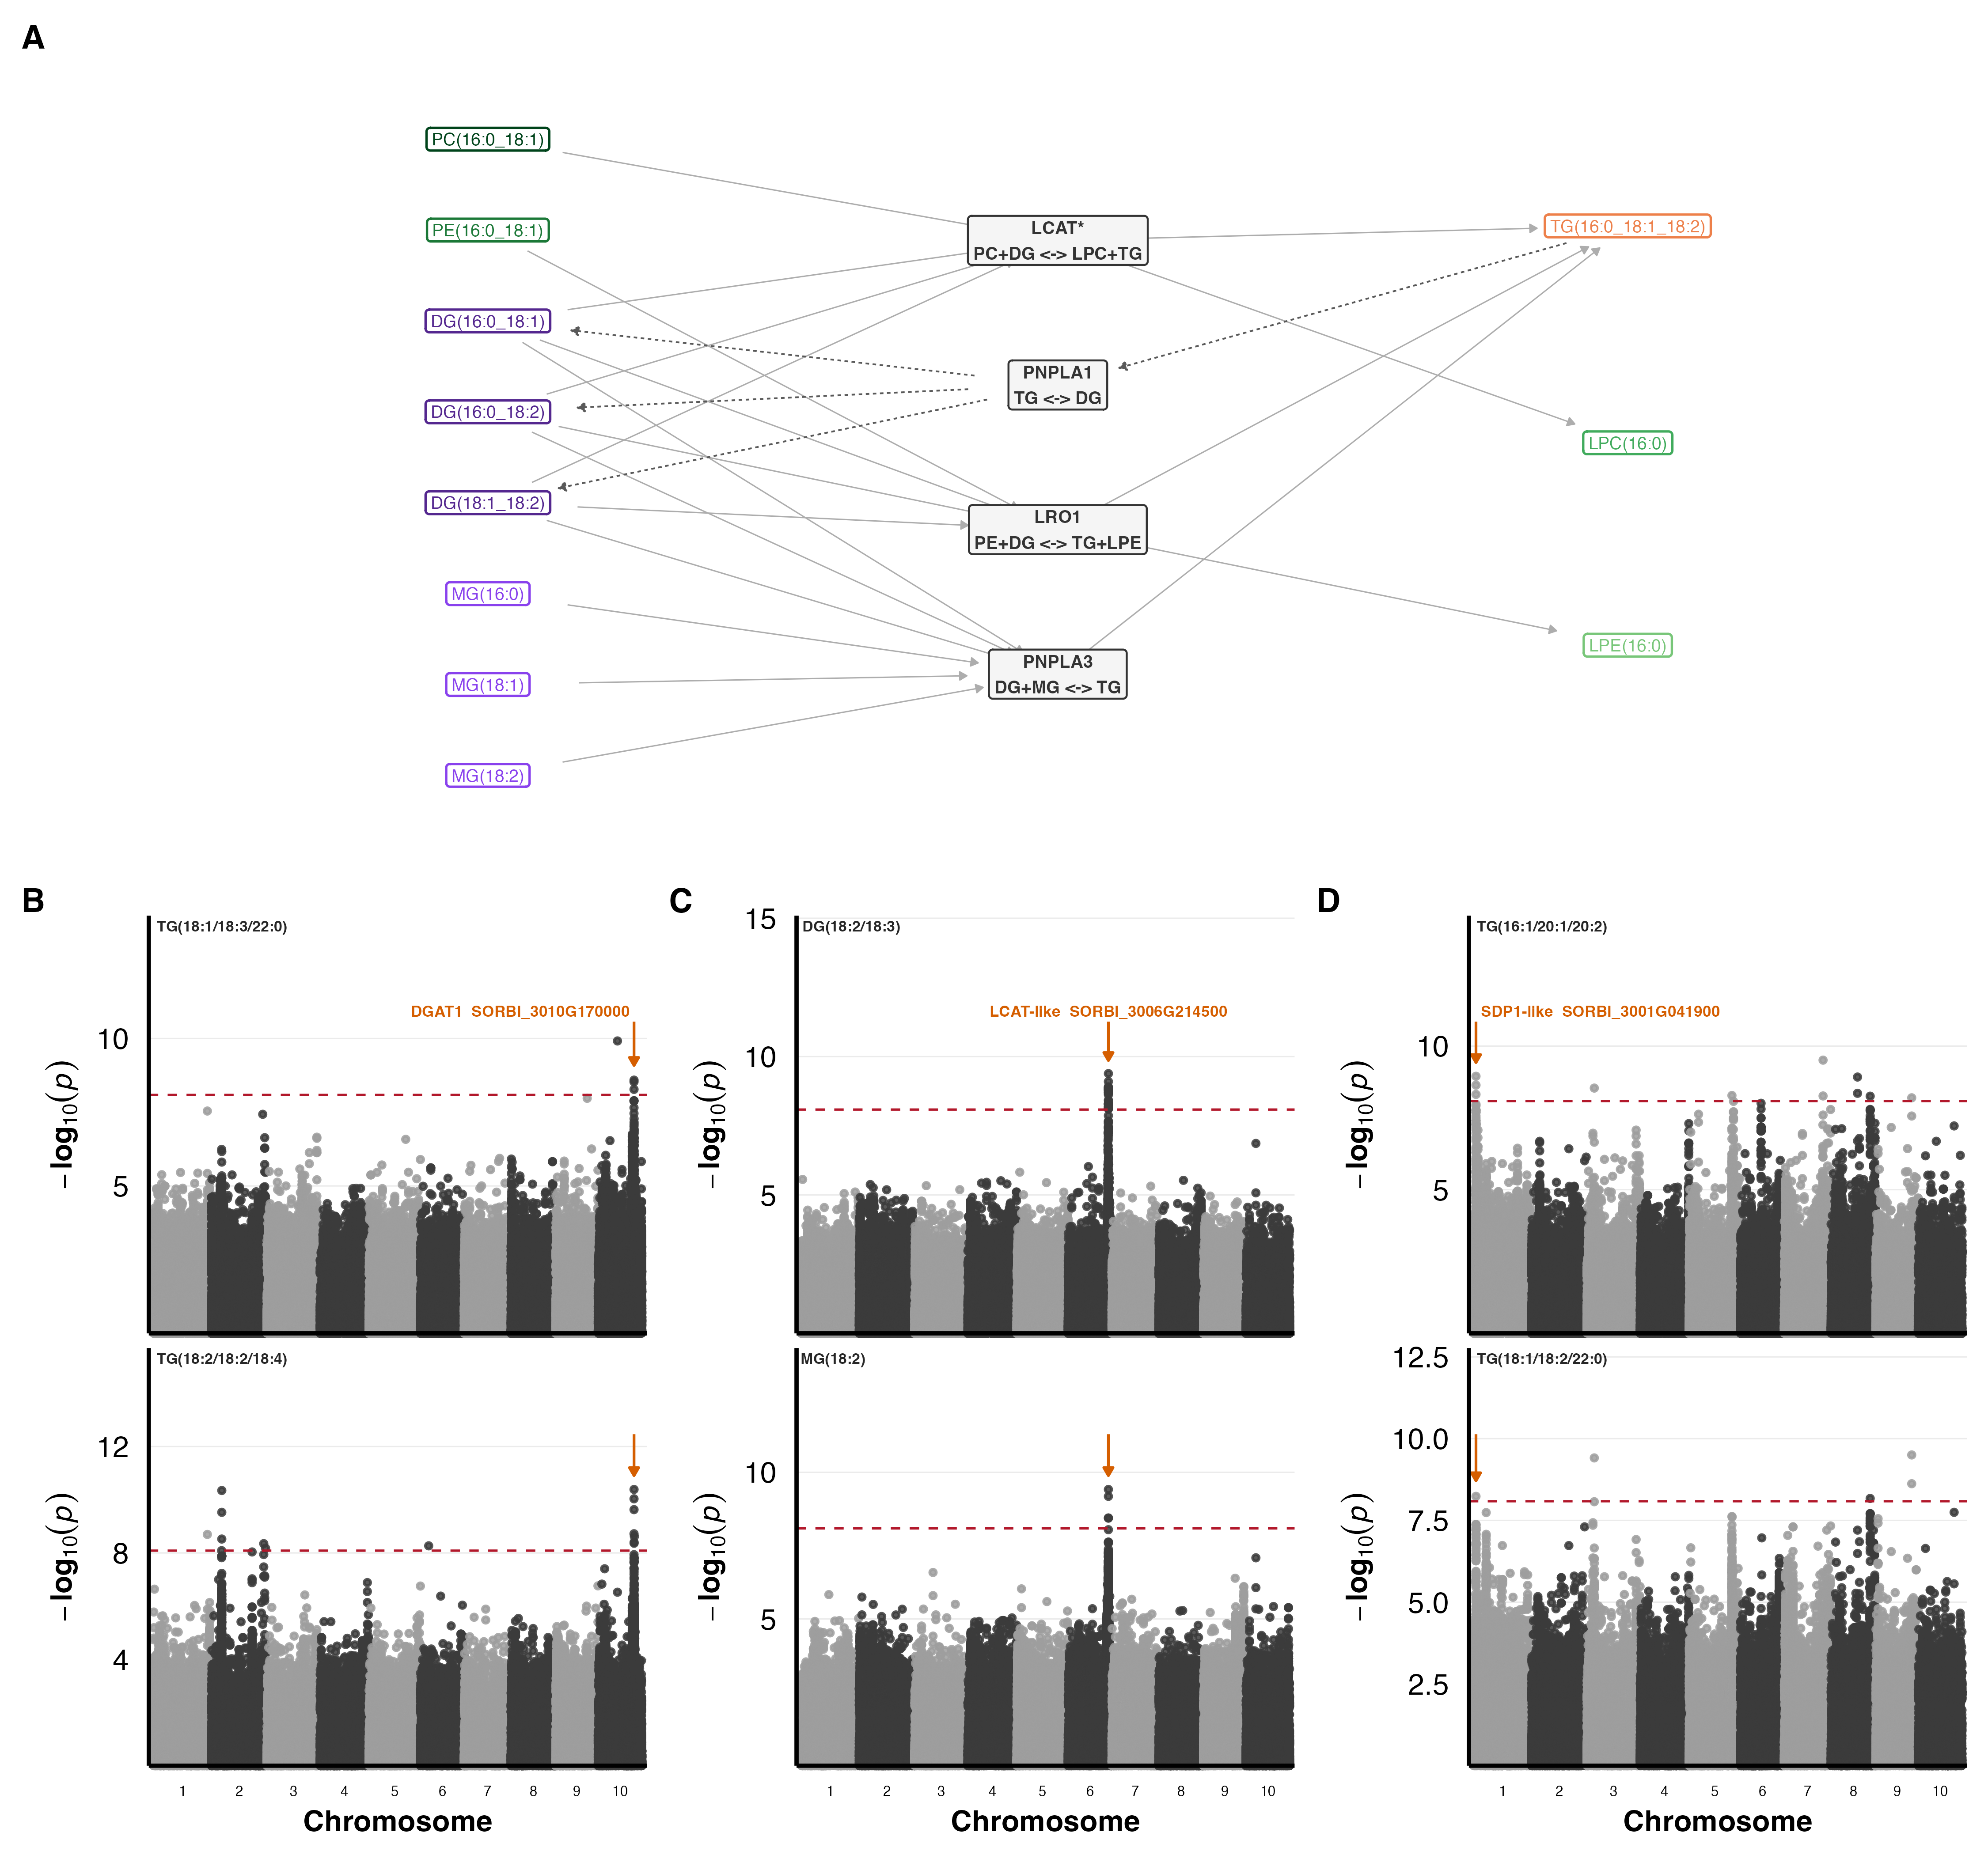
\includegraphics[width=\textwidth]{fig/main/Figure5_LINEX.png}
\caption{\textbf{Candidate lipid reaction branches and the GWAS support for them.}
\textbf{(A)} LINEX-enriched lipid reaction subnetwork connecting candidate reactions to their substrate and product lipid species. Central reaction nodes depict hypothesized LCAT-like acyl editing, PNPLA1-mediated TG$\rightarrow$DG lipolysis, LRO1-mediated acyl transfer between PE/DG and TG/LPE, and PNPLA3-associated DG/MG$\rightarrow$TG re-esterification; arrows show reaction direction, dashed arrows run right to left, and boxed labels give representative lipid species coloured by class. All four reactions were retrieved from the LINEX2 network; the enzyme label on the acyl-editing branch, marked LCAT*, was assigned from reaction specificity rather than returned by LINEX2.
\textbf{(B--D)} GWAS support for the three branch-supporting candidate genes under LIN, two associated traits per gene: \textbf{(B)} \textit{DGAT1} (\texttt{SORBI\_3010G170000}), \textbf{(C)} an LCAT-like gene (\texttt{SORBI\_3006G214500}), and \textbf{(D)} an SDP1-like lipase (\texttt{SORBI\_3001G041900}). An orange arrow marks the lead SNP at each candidate locus, and the gene is named once above the arrow in the top plot of its column; each plot is identified by the trait in its upper-left corner. Red dashed horizontal lines mark the Bonferroni genome-wide threshold, and point shading alternates by chromosome. The reaction-balance scores for these branches are given in Supplementary Table~S9 (reaction balance) rather than shown here, because they are a CTL--LIN contrast.}
\label{fig:Fig4_linex_rewiring_abc}
\end{figure*}

\subsection*{An interactive SoLD Shiny application enables exploration of lipid and GWAS results}

The SoLD web server provides a clean and readable browsing experience for exploring lipid phenotypes and their genetic associations across two field environments (Fig.~\ref{fig:Fig5_shiny_app}A). Traits can be examined at three resolutions: individual species, class-level sums, and inter-class ratios \citep{Fahy2009LipidMapsClass}, as well as hierarchical filtering by LIPID MAPS category and species. Exploratory and multivariate modules (data preview, boxplots, volcano plots, correlation and network views, heatmaps, PCA, t-SNE/UMAP) are paired with two genetic modules: (i) GWAS, which shows trait-specific associations, and (ii) Gene Hits, which aggregates recurrent candidate genes under user-defined dataset, trait-type, lipid-class, and significance settings. Furthermore, a Genotype module supports experimental design by identifying accessions within specified lipid value ranges.

\begin{figure*}[!t]
\centering
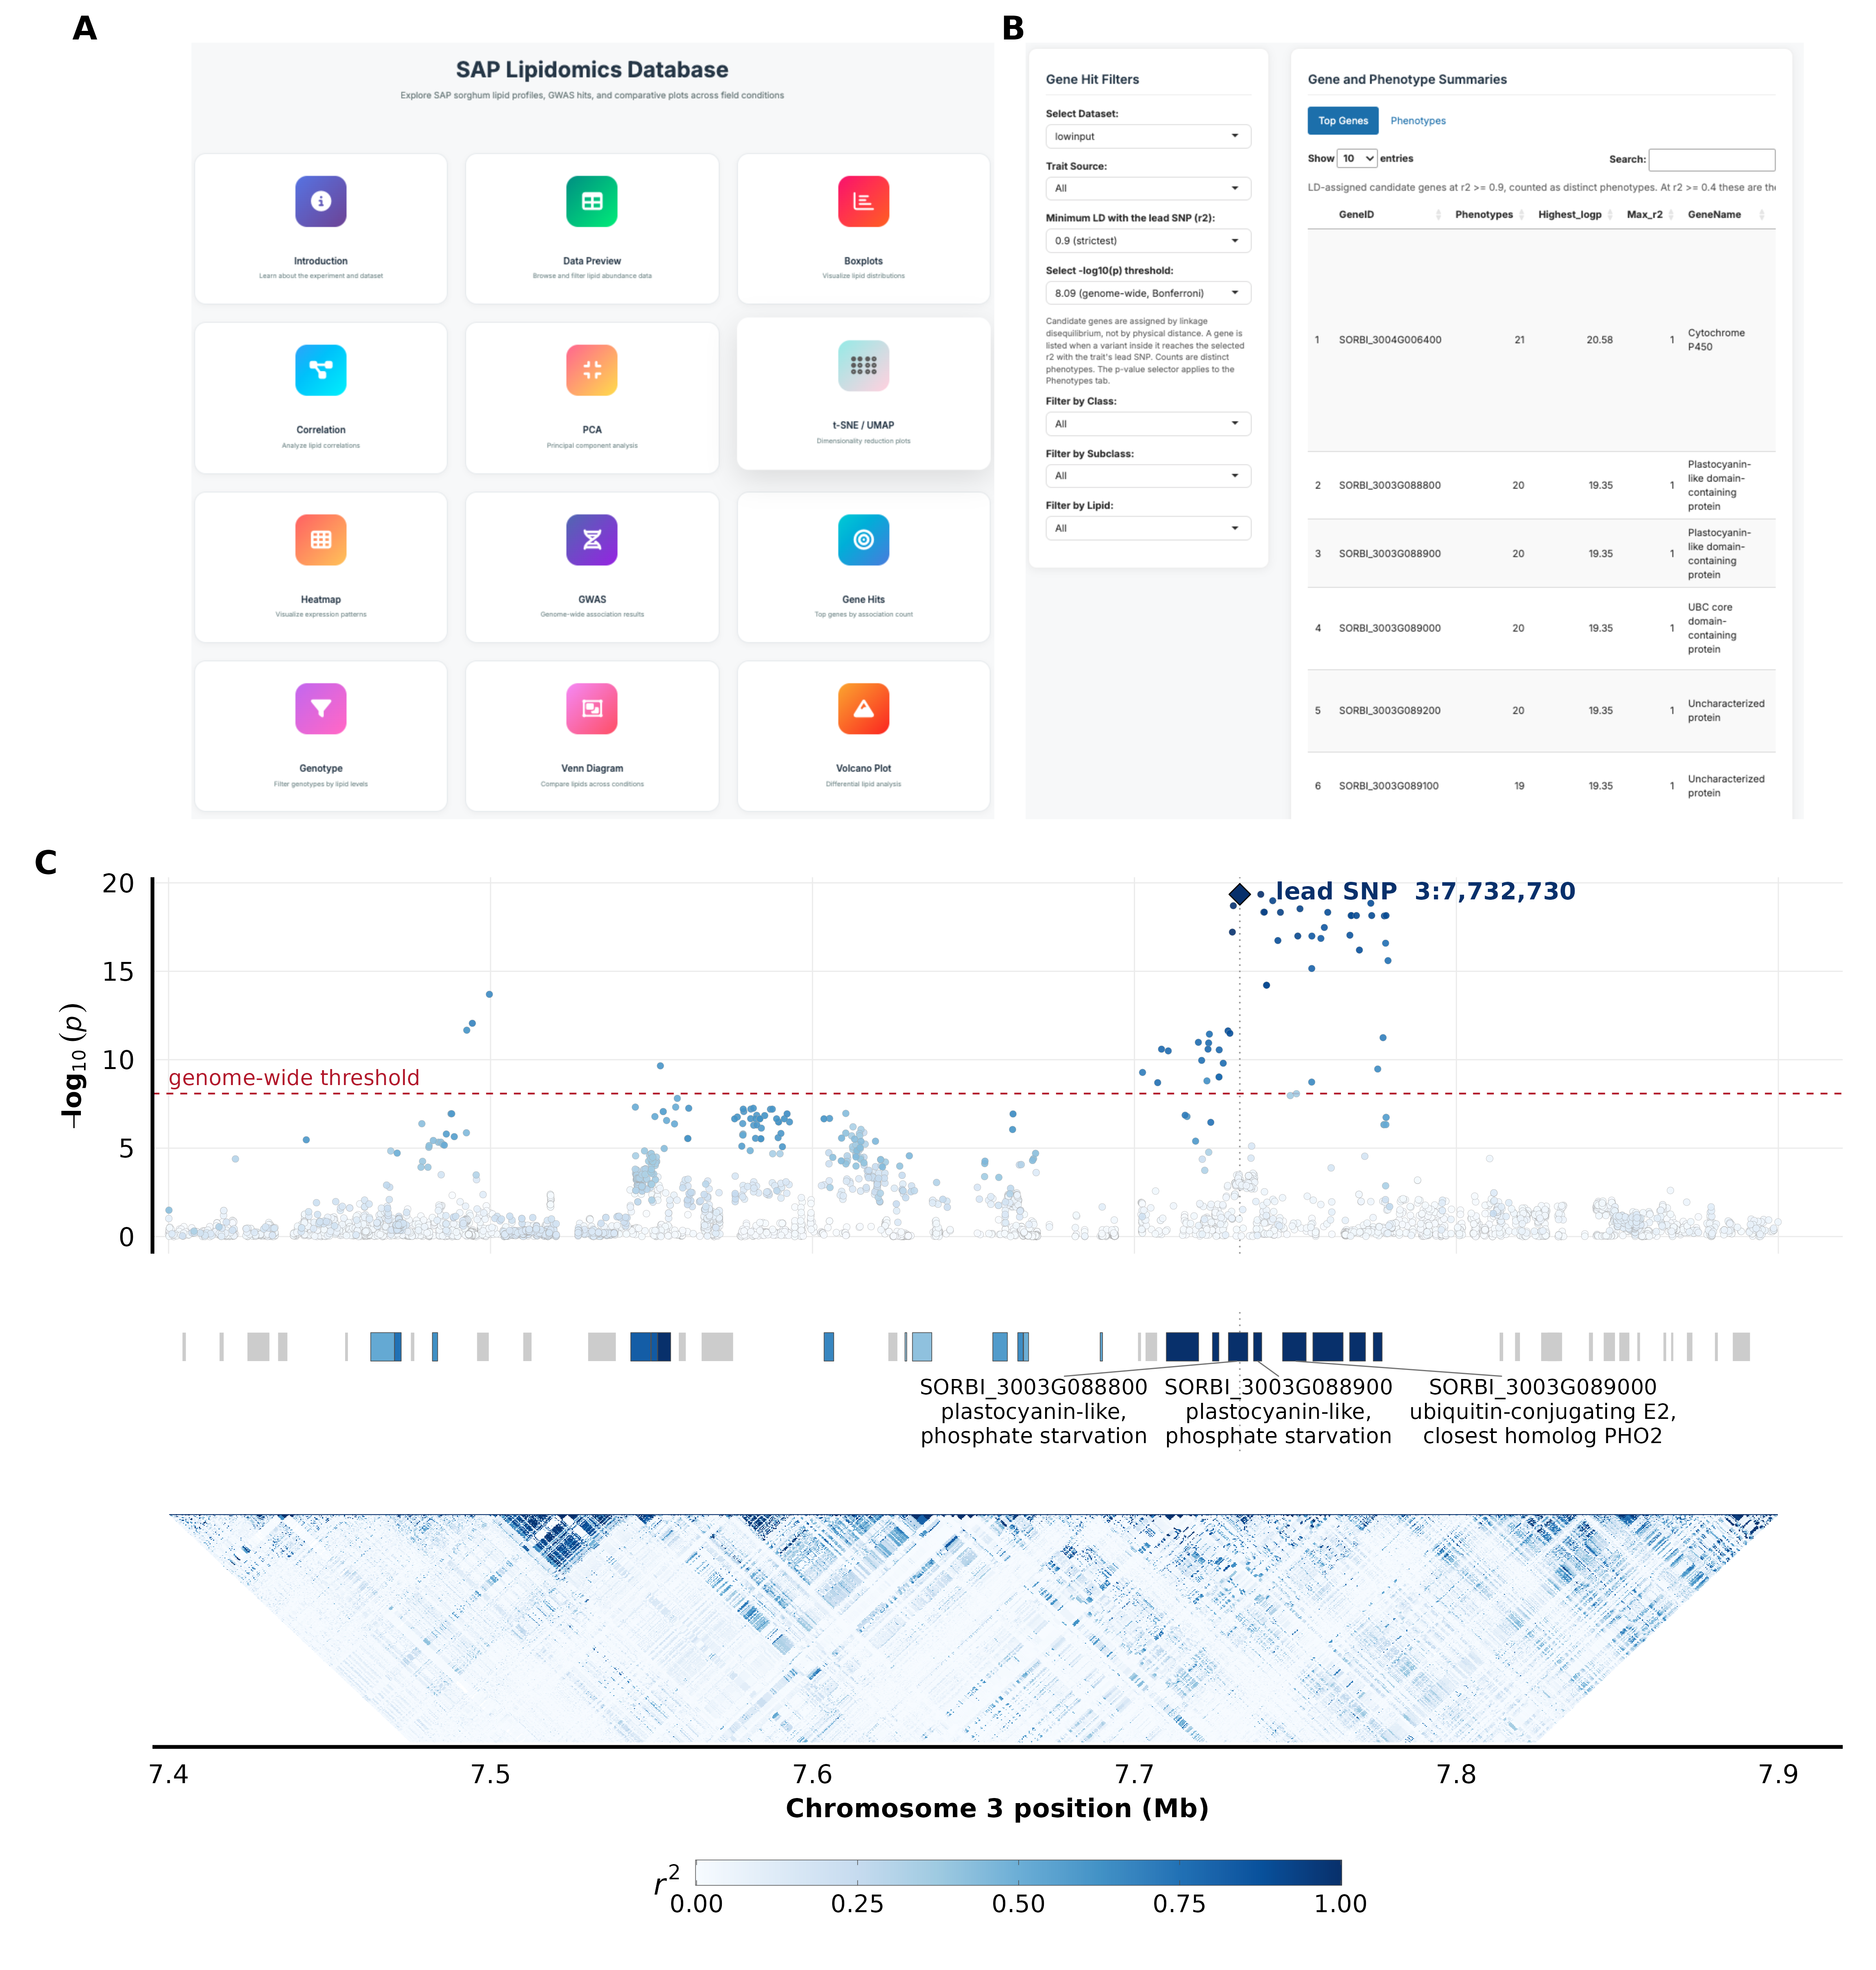
\includegraphics[width=\textwidth]{fig/main/Figure7_Shiny_App.png}
\caption{\textbf{SoLD Shiny app and the chromosome~3 candidate block under LIN.}
(A) The homepage of the SoLD Shiny app with a list of features. (B) Gene Hits module under the LIN dataset, all trait sources, the genome-wide threshold, and the strictest LD setting (r$^2 \geq 0.9$), ranking candidate genes by the number of distinct phenotypes each recurs in. (C) Regional view of the chromosome~3 locus that the top of that table points to, over 7.40--7.90~Mb for the LIN fatty-acid class sum. Top, every GWAS SNP as $-\log_{10}(p)$, coloured by its r$^2$ with the lead SNP, with the LIN Bonferroni threshold dashed and the lead SNP as a diamond; a second SNP at 3:7{,}739{,}242 ties it at $p = 4.46\times10^{-20}$. Middle, the 49 annotated genes in the window, coloured by the highest r$^2$ any variant inside them reaches with the lead SNP, which is how candidate genes are assigned throughout; grey genes carry no variant at r$^2 \geq 0.4$. Three of the five block genes are labelled, the other two being uncharacterised. Bottom, pairwise r$^2$ between variants less than 150~kb apart. All three tiers share one r$^2$ scale.}
\label{fig:Fig5_shiny_app}
\end{figure*}

Also, the interface allows for easy tracing of traits to candidate genes through the combination of filtering, plotting, and gene summaries. In the \emph{Gene Hits} module (LIN dataset; all trait sources; genome-wide threshold; strict LD, $r^2 \geq 0.9$), 1,291 candidate genes are output and ranked by the number of phenotypes in which they recur (Fig.~\ref{fig:Fig5_shiny_app}B). The top gene is a chromosome 4 cytochrome P450 (\texttt{SORBI\_3004G006400}), recurring in 14 phenotypes. Next are five adjacent chromosome 3 genes. Each carries a variant in perfect linkage disequilibrium ($r^2 = 1$) with the most significant SNP at the locus, recurs in the same 11 phenotypes, and shares the same association ($p = 4.46 \times 10^{-20}$), which places them above a sixth gene, \texttt{SORBI\_3003G406600} at 71.4~Mb on the same chromosome, that matches their phenotype count but not their $p$-value. These are one class sum (free fatty acids), one species, FA(22:1), and nine class ratios. In the 500~kb window (7.40--7.90~Mb) around these genes, the association is concentrated in $\sim$7.70--7.78~Mb, which carries 48 of the 52 genome-wide significant SNPs in the window, the remaining four lying near 7.49 and 7.55~Mb (Fig.~\ref{fig:Fig5_shiny_app}C), and 26 of the 49 genes in the window were not selected ($r^2 < 0.4$). Three of the five block genes are well characterized. \texttt{SORBI\_3003G088800} and \texttt{SORBI\_3003G088900} are near-identical neighbors, closest to rice \textit{OsLPR2} and \textit{OsLPR1} (76\% and 75\% amino-acid identity), which encode multicopper oxidases of the LOW PHOSPHATE ROOT family that govern the root meristem response to phosphate deficiency. The third gene, \texttt{SORBI\_3003G089000}, whose closest annotated Arabidopsis relative is UBC24/PHO2, acts as a negative regulator that limits phosphate uptake and root-to-shoot translocation. Two arms of the phosphate-starvation response, sensing at the root and restraint of transport, therefore fall within a single LD block detected under LIN. Thus, the SoLD Shiny app brings together lipid phenotypes, their associations, and LD-supported candidate genes, enabling direct recovery and inspection of loci (e.g., the chromosome 3 block), comparison of compositional and multivariate views across two trials, and selection of accessions by lipid content for follow-up experiments.

\section{Discussion}

The two trials differ in lipid composition at the class level. Lipid-trait loci, in contrast, were largely distinct between them. We first link the lipidome changes to trial conditions, then discuss candidate genes, and finish with the near-absence of shared loci between trials, which points to different genes acting on the same pathways in each environment. All GWAS results returned far more candidate genes than could be interpreted, with 1,062 for individual lipids and 54 for class sums and ratios under CTL, compared to 4,370 and 385 under LIN, because a single significant SNP tags every gene in its LD block. Two filters reduced these to the set discussed below. Most candidates fall within ontology terms passing the LD-aware permutation null, supported by both enrichment and association (Supplementary Table~S7, genes in enriched terms). A second set comes from the LINEX reaction network, retaining genes mapped to branches flagged as remodeled between trials. These two approaches yield different types of candidates because enrichment clusters genes by function, while the reaction network maps them to the reactions connecting the lipid classes that showed changes. However, two caveats apply. First, gene functions are inferred by orthology to characterized genes in other species. Second, candidates come from LD blocks, so most associated regions contain several genes that should also be taken into account for validation.

\subsection*{Integrated interpretation of lipidome remodeling across contrasting field trials}

The two most prominent changes in LIN are a decrease in SQDG and an increase in TG. The accumulation of TG is commonly associated with low temperatures, drought, oxidative stress, and nutrient-driven carbon reallocation, suggesting a shift towards increased storage within the LIN signature \citep{Tan2018, Yan2025, Pfaff2020}. 

The median LIN balances are higher than CTL for every ratio in which TG is the numerator, TG/SQDG (4.1$\times$), TG/MG (2.4$\times$), TG/MGDG (2.1$\times$), TG/DG (1.8$\times$), and TG/PE (1.7$\times$), so TG rises against every other class (Supplementary Table~S4, ratio statistics). DG rises less than TG but more than MG, giving DG/MG 1.3$\times$, while DG/PS falls to 0.32$\times$ because PS rises further still.

The median LIN balances are higher than CTL for TG/DG (2.2$\times$), TG/MGDG (2.7$\times$), TG/SQDG (3.6$\times$), and TG/PE (1.3$\times$). The exception is TG/MG (0.74$\times$), reflecting a faster rise in MG. DG shifts oppositely as DG/MG is 0.34$\times$ and DG/PS is 0.13$\times$. Correlations also change. PS--TG switches from negative in CTL ($r=-0.26$) to positive in LIN ($r=+0.43$), a strong sign reversal (Supplementary Table~S4, CLR correlation delta). Additionally, LINEX reactions add to these results. TG-producing branches shift toward products under LIN, while TG$\rightarrow$DG hydrolysis shifts toward substrate, collectively favoring TG over DG (Supplementary Table~S9, reaction balance). These class-level balances together suggest a reorganization of DG supply and TG synthesis and mobilization, though direct measures of enzyme activity are needed. Both arms contain LIN candidates. \textit{DGAT1} (\texttt{SORBI\_3010G170000}) acylates diacylglycerol to triacylglycerol and falls within a repeatedly mapped chromosome 10 crude-fat QTL in sorghum \citep{Boyles2017DGAT1, Yen2008DGAT}. The reverse (hydrolytic) step is \texttt{SORBI\_3001G041900}, an SDP1-clade lipase. In Arabidopsis, SDP1 hydrolyses triacylglycerol to diacylglycerol and free fatty acid and accounts for most TG breakdown during reserve mobilization \citep{Kelly2011SDP1L}. This locus clusters with \textit{SbSDP1-L} in the sorghum lipase phylogeny \citep{Sapara2024PLA}.


Another change involves the balance among phospholipid headgroups. PS increased against every class it was tested against (Supplementary Table~S4, ratio statistics), and the PS--PC correlation flipped from positive in CTL ($r=+0.43$) to negative in LIN ($r=-0.34$), the largest shift among class pairs (Supplementary Table~S4, CLR correlation delta). PE showed the largest increase in mean double-bond number of any class, although the species detected differ slightly between trials, and this is a composition measure rather than a direct account of acyl editing. Comparable shifts in headgroup proportions, membrane unsaturation, and lysophospholipid pools are reported under cold, nutrient, oxidative, and water limitation, where they accompany changes in membrane fluidity, lipid repair, signaling, and remobilization \citep{Hou2016, Rawat2021, Yan2025, Zhang2020}. The balance between the lysophospholipid classes also shifted, with LPC/LPE dropping to 0.48-fold in LIN (Supplementary Table~S4, ratio statistics), driven by LPE rising from 0.0065\% to 0.0139\% of total signal while LPC was essentially unchanged (Supplementary Table~S4, composition \%TIC). PS and the lysophospholipids each contribute under 0.2\% of TIC, so these are large proportional changes on small pools. The annotation is also shallow, with four LPC species under CTL and three under LIN and a single LPE species in both, so the shift cannot be read as evidence about phospholipase activity.

These changes do not indicate phosphate conservation, nor a headgroup swap. Under phosphate limitation, phospholipids are degraded to release phosphate and replaced by glycolipids, raising SQDG/DGDG and lowering phospholipids \citep{Essigmann1998, Hartel2000, Jouhet2004, KellyDormann2002, Pfaff2020}, however, neither occurs here. On the CLR scale, SQDG drops most ($-0.942$, $0.39\times$), galactolipids drop less (MGDG $0.77\times$, DGDG $0.85\times$), and PG shows no change (Supplementary Table~S4), so the two anionic thylakoid lipids decline together rather than substitute (3.13\% to 1.72\% of TIC). Phospholipids hold steady (30.3\% to 30.2\% of TIC) while glycolipids fall (47.5\% to 43.5\%), increasing the phospholipid:glycolipid ratio. Additionally, all phospholipids increase relative to SQDG (PC $2.07\times$, PE $2.41\times$, PG $2.54\times$; Supplementary Table~S4). PC salvage via deacylation would increase LPC, but LPC does not accumulate ($0.87\times$ CLR), so that route does not explain the modest PC decline. Overall, the lipidome suggests a smaller plastid lipid fraction with a disproportionate loss of SQDG. Because SQDG is the only sulfur-containing plastid lipid, this pattern is consistent with constrained sulfolipid synthesis. The LIN GWAS included two SQD2-like loci (\texttt{SORBI\_3003G076900}, \texttt{SORBI\_3002G000600}), though they were implicated via fatty-acid traits, not SQDG. In the absence of sulfur, chlorophyll, or thylakoid measurements, and considering the other reported LIN vs CTL differences, the lipidome data alone constrain conclusions about the underlying mechanism. Thus, the LIN lipidome is best understood as a redistribution among plastid, phospholipid, lysophospholipid, and neutral-storage pools, supported independently only by the GWAS.

\subsection*{Genetic control of lipid variation is stronger under LIN and largely trial-specific}

These compositional changes coincide with a shift in how strongly lipid variation reflects genotype. Under CTL, the median $h^2$ was near zero (11/164 species excluded zero), while under LIN the median $h^2$ was 0.170 (53/164 excluded zero), with $h^2$ higher under LIN for 131 species versus 21 under CTL. This difference persisted after conditioning on population structure and after removing any race group or 20\% of accessions. Low heritability for individual leaf metabolites in a single field environment is usual rather than exceptional. Mean broad-sense heritability across 76 leaf metabolites in a 135-line wheat panel was 0.25, with genotype-by-location variance twice the genetic variance \citep{Matros2017}, and 25 to 40\% of leaf mass features in a 282-line maize panel fell below $H^2=0.2$ \citep{Zhou2019}. Our values are genomic heritabilities from a marker-based relationship matrix, so they capture only the additive variance tagged by markers and are expected to sit below broad-sense estimates from replicated designs. CTL is therefore better read as a low-genetic-variance environment. A similar one-sided pattern holds for ancestry, though effects are small. No lipid-class sum was associated with botanical race in either trial (smallest $q=0.479$, $\varepsilon^2 \leq 0.027$). No species was significant under CTL, whereas nine were under LIN, eight by marker-based genetic cluster alone and one by cluster and by race, led by $\beta$-sitosterol ($\varepsilon^2=0.095$, $q=7.7\times10^{-5}$) and PS(18:0/18:2) ($\varepsilon^2=0.088$, $q=1.2\times10^{-4}$). Thus, ancestry explains little in either trial, and a detectable signal appears only under LIN. Moreover, the GWAS mapping results show the same asymmetry, with traits that have higher heritability being simpler to map, so the longer LIN candidate list likely indicates higher $h^2$ rather than a greater number of genes.

Candidate loci were largely trial-specific. The two candidate sets overlapped more than chance ($2.07\times$), but a single association tags every gene in its linkage block, so one shared region is counted once for each gene it contains. Counting shared 250 kb regions instead of shared genes removes the excess for individual lipids, from 282 shared genes ($2.07\times$) to 153 shared regions ($1.05\times$, $p=0.22$). Class sums and ratios share no gene and no region between trials at all, so the excess is confined to individual species and does not survive the collapse of linkage in either layer. Sharing a region is also not the same as sharing a trait. Of the 291 genes recovered in both trials, none is a candidate for the same trait in both, even though 13 traits are significantly associated in both (Supplementary Table~S31, shared ranked). Because the trials differ by year, field, and batch, as well as nutrients, these results do not isolate a genotype-by-nutrient effect, and testing that would require repeating the nutrient contrast within a single year.

\subsection*{A cold-induced MADS regulator is associated with fatty-acid traits under LIN}

Developmental timing and cold response might be studied on \texttt{SORBI\_3003G406800}, a MADS-box transcription factor associated with fatty-acid traits under LIN for FA(22:1), PC(18:2\_20:4), the fatty-acid class sum, and eight FA-to-class ratios. The only GO term it carries that passes the LD-aware null is \textit{DNA binding}, drawn from a background of 1,166 genes and too broad to add anything, so the case for it rests on its associations and on prior work rather than on enrichment. It also shares every one of those associations with seven other genes in the same LD block, so the mapping does not single it out. Multiple studies support its cold-response role. In sorghum, this gene is induced in cold, and it is a hub in the early shock co-expression module \citep{Kurt2026ColdSorghum}. Its functional homolog in maize, \textit{ZmMADS69}, a flowering-time locus, regulates ZmRap2.7/\textit{ZCN8} and was selected during tropical-to-temperate adaptation \citep{Liang2019ZmMADS69}.

LIN was planted earlier to expose the plants to cold during establishment, so a cold-induced gene linked to fatty-acid traits fits the treatment. Cold acclimation also involves acyl-chain remodeling to maintain membrane fluidity \citep{Tan2018, Zhang2020}. However, LIN also differs from CTL in nitrogen, phosphorus, and chemicals, so temperature cannot be isolated. A MADS-box flowering-time regulator may instead reflect a developmental-stage shift at sampling rather than lipid regulation, which this design cannot differentiate. Earlier planting also changes the photoperiod and temperature a plant experiences at each stage, so a flowering-time locus would be expected to differ between the trials, whether or not it acts on lipids. Thus, the locus ties earlier planting to fatty-acid variation, though whether that runs through cold response, developmental timing, or both is not resolved here.

\subsection*{Nitrate transporters are the remaining nitrogen-related candidates under LIN}

Nitrogen transport enters the LIN candidate set through two GO enrichments. The first is specific but narrow. \textit{Nitrate transmembrane transporter activity} and \textit{nitrate transmembrane transport} are enriched in the fatty-acid set, the stronger at $25\times$ enrichment ($q_{\mathrm{LD}}=0.045$). Both are counted across two 250~kb intervals, but the two lead SNPs are 136~kb apart and fall either side of a bin boundary, so this is better read as one locus than two. The second enrichment is broad but distributed, covering \textit{transmembrane transporter activity} and \textit{transmembrane transport}.

The nitrate terms are driven by \texttt{SORBI\_3004G009400} (NRT2.1-like, high-affinity) together with two adjacent genes of the same family, \texttt{SORBI\_3004G009200} and \texttt{SORBI\_3004G009500}, all three within a 250~kb interval on chromosome~4. \texttt{SORBI\_3004G009400} is the best supported of the three and is associated with FA(22:1), the fatty-acid class sum, and two oxidised fatty acids, 13S-HOTrE and 13-keto-9Z,11E-octadecadienoic acid. That interval tags 23 LIN candidate genes in total, so LD does not single out the transporters within it. In maize, NRT2.1 requires NAR2.1, and its capacity varies along the root with plasma-membrane H$^+$-ATPase activity \citep{Lupini2016NAR2, Sorgona2011Nitrate}.

Two additional NPF/NRT1 transporters, \texttt{SORBI\_3008G081400} and \texttt{SORBI\_3001G133900}, appear in the broad transport terms. \texttt{SORBI\_3008G081400} is recovered in both trials (seven TGs under CTL, five of them palmitate-containing; FA(22:1), TG(18:1\_18:2\_18:2) and 11,14,17-eicosatrienoic acid under LIN). Its closest Arabidopsis homolog is NPF4.6/NRT1.2/AIT1, which transports both nitrate and abscisic acid without the two competing as substrates \citep{Kanno2013NPF46}. The same protein interacts with PHOSPHOLIPASE D$\alpha$1 at the plasma membrane, and \textit{PLD$\alpha$1} is epistatic to \textit{NRT1.2} in ABA responses \citep{Li2020NRT12PLD}. The homolog therefore sits at a junction of nitrate transport, ABA transport and phospholipase D activity, which is a plausible point of contact between nitrogen status and membrane lipid turnover, although the PLD$\alpha$1 interaction was characterized in seed germination rather than in leaves. \texttt{SORBI\_3001G133900} associates with one lipid, TG(14:0\_18:2\_18:3), and its rice ortholog OsNPF2.4 mediates low-affinity nitrate root-to-shoot transfer \citep{Xia2015NPF24}. Thus, these three transporters are the most promising nitrogen-related candidates in the LIN set for follow-up work.

\subsection*{Phosphate and sulfur candidates recovered under LIN}

Under LIN, the term cellular response to phosphate starvation is enriched across most class-sum strata, and in the SQDG traits its three genes are \texttt{SORBI\_3001G028500} on chromosome 1, and \texttt{SORBI\_3003G088800} and \texttt{SORBI\_3003G088900} on chromosome 3. \texttt{SORBI\_3001G028500} encodes an SPX-domain phosphate-status signaling protein and is associated with FA(22:1), the fatty-acid class sum, and the SQDG-to-fatty-acid ratio. Like rice OsSPX4, which negatively regulates phosphate signaling through its interaction with PHR2, it may regulate phosphate-starvation responses \citep{Lv2014SPX4}.

The two chromosome 3 genes sit in one of the strongest signals recovered under LIN ($p = 4.46\times10^{-20}$, 52 significant SNPs), associated with FA(22:1), the free fatty acid class sum, and nine class-ratio traits. This is the same block recovered through the \emph{Gene Hits} module above. \texttt{SORBI\_3003G088800} and \texttt{SORBI\_3003G088900} are separated by 1.8 kb and are closest to the rice \textit{OsLPR2} and \textit{OsLPR1}, the multicopper oxidases of the LOW PHOSPHATE ROOT family, which control the root meristem response to phosphate deficiency. In rice, the family has expanded to five genes, \textit{OsLPR1--5}, within 65 kb of chromosome 1, of which \textit{OsLPR3} and \textit{OsLPR5} are induced by Pi deficiency \citep{Cao2016OsLPR}, so the sorghum pair is closest to the non-induced members. The same block carries a PHO2-family ubiquitin-conjugating E2, \texttt{SORBI\_3003G089000}. PHO2/UBC24 is a negative regulator that limits phosphate uptake and root-to-shoot transport. The gene \textit{pho2} overaccumulates Pi through a nonsense mutation in \textit{UBC24}, and \textit{PHO2} is miR399-cleaved under phosphate deficiency \citep{Aung2006PHO2}. PHT1 transporters and PHOSPHATE TRANSPORTER TRAFFIC FACILITATOR1 act downstream of PHO2 \citep{Huang2013PHO2}, and in Arabidopsis the RING-type E3 ligase NITROGEN LIMITATION ADAPTATION partners with UBC24 to ubiquitinate PT2 \citep{Park2014NLA}, a link that matches our design because LIN reduced both N and P. The block holds five genes in all, the remaining two being a WD40-repeat protein (\texttt{SORBI\_3003G089100}) and a glutamyl-tRNA amidotransferase subunit (\texttt{SORBI\_3003G089200}), neither of which belongs to an enriched term. Because every gene in the block is tagged by the same signal, the association identifies the region rather than any one gene within it.

Two transporters are included via the candidate list rather than by enrichment, and both map only to the general transport terms (not shown in Fig.~\ref{fig:go_bp_main}). \texttt{SORBI\_3006G244000}, a STAS-domain protein placed in the SULTR3 family by homology, is associated with three species, TG(14:0\_18:3\_18:3) across 40 significant SNPs, TG(12:0\_18:2\_18:3) across 11, and PC(18:2\_20:4) across four. In Arabidopsis, SULTR3 proteins localize to the chloroplast envelope and mediate chloroplast sulfate uptake \citep{Chen2019SULTR3}. Because SQDG is a plastid lipid whose sulfur-containing head group depends on plastid sulfate import and reduction, SULTR3 sits on the sulfur-supply route to SQDG. Phosphate limitation typically raises SQDG by replacing phospholipids, yet SQDG was depleted under LIN, which makes constrained plastid sulfate supply a hypothesis worth exploring. \texttt{SORBI\_3002G116100} encodes a PHT1-family H$^+$/Pi cotransporter whose closest characterized rice relative is OsPT4 (\textit{OsPht1;4}), affecting phosphate accumulation and embryo phosphate mobilization \citep{Ye2015OsPT4,Zhang2015OsPht14}. Its five traits are four TGs and one PC rather than phospholipids, which does not fit a simple phospholipid-to-glycolipid replacement under phosphate limitation. Thus, these loci are prioritized for functional validation for LIN associated phenotypes.

\subsection*{A TIFY/JAZ region enriched under LIN is also recovered under CTL for different lipids}

Under LIN, three TIFY-domain genes on chromosome 1 (\texttt{SORBI\_3001G259300}, \texttt{SORBI\_3001G259400}, \texttt{SORBI\_3001G259600}) drive the enrichment of the regulation of defense response, regulation of the jasmonic acid mediated signaling pathway, and response to wounding, all from the AEG trait class. Each of the three terms is carried by a single 250~kb interval, so they are reported in Supplementary Table~S17 rather than shown in Fig.~\ref{fig:go_bp_main}, which is restricted to gene sets spanning at least two independent intervals. All three genes associate with AEG(o-15:2\_15:0) and PC(14:0\_18:3), and \texttt{SORBI\_3001G259400} and \texttt{SORBI\_3001G259600} additionally associate with 11,14,17-eicosatrienoic acid. The same region is also recovered under CTL, but for different lipids and without a corresponding enrichment. There, \texttt{SORBI\_3001G259400} and \texttt{SORBI\_3001G259600} are candidates for the nine TG species, seven of which contain 16:0. \texttt{SORBI\_3001G259700} is a candidate for four of those nine, and none of the genes is a candidate for any TG under LIN.

TIFY/JAZ proteins repress jasmonate signaling, and jasmonate slows growth while redirecting metabolism toward defense and repair \citep{Larrieu2016JA}. Jasmonate is made from $\alpha$-linolenic acid (18:3) released from plastid galactolipids, and the LIN traits include PC(14:0\_18:3), which carries that precursor, and a free C20:3. Nitrogen, phosphorus, and temperature all differ between CTL and LIN, and each has a documented connection to jasmonate signaling. Nitrate signaling can act through NIN-LIKE PROTEIN 7 to activate \textit{JAZ1}, while jasmonate can restrain nitrate-driven growth through COI1-dependent JAZ1 degradation \citep{Pu2025JAZ1}. Phosphate deficiency can also increase jasmonate and jasmonoyl-isoleucine levels and enhance herbivory resistance \citep{Khan2016PiJA}. Low temperature provides another relevant stress context, as most \textit{OsTIFY} genes respond to cold in rice \citep{Ye2009TIFYRice}, and TIFY-family genes have also been implicated in cold responses in pepper and sweet orange \citep{Wang2023CaTIFYCold,Zhang2026TIFYOrange}. The whole pathway is a plausible point of contact for future studies. However, LD does not isolate the TIFY genes. The same significant SNPs also tag an SPX domain-containing protein (\texttt{SORBI\_3001G259100}, explained above), a glycosyltransferase, a translation initiation factor, and several uncharacterized genes in the same block. The whole region might be of interest for future studies.

\section*{Conclusion}

SoLD is a population-scale lipidomics web resource for SAP, profiling 266 annotated lipid species across two contrasting fields. Compared with CTL, the LIN lipidome showed four population-wide shifts: SQDG depletion, TG enrichment, a PS-centered phospholipid redistribution, and an LPC/LPE balance shifted toward LPE. These were independent of botanical race and genome-wide genetic structure. Genomic heritability was also higher under LIN with a median near zero under CTL compared to 0.170 under LIN. The increase reflects more genetic variance rather than less experimental noise, so more of the lipidome can be mapped under LIN than CTL.

GWAS returned far more candidate genes than could be interpreted. Under CTL we obtained 1,062 for individual lipids and 54 for class sums and ratios, and 4,370 and 385 under LIN. Two filters reduced these numbers based on ontology terms, passing an LD-aware permutation null and genes mapped onto LINEX reaction branches. The two filters return different kinds of candidates. Enrichment groups genes by function, whereas the reaction network assigns them to the specific reactions linking the lipid classes that changed between trials. Both arms of DG--TG cycling are recovered by this route, including \texttt{SORBI\_3010G170000} (\textit{DGAT1}) for polyunsaturated TGs and an SDP1-like lipase for the reverse reaction. GO enrichment identifies nutrient and cold candidates. \texttt{SORBI\_3006G244000}, a SULTR3-family chloroplast sulfate transporter, offers a potential mechanism for the SQDG decline that the canonical phosphate-starvation response does not explain. Furthermore, the strongest recurrence under LIN is a chromosome 3 block carrying two LOW PHOSPHATE ROOT homologues, which share an enriched \textit{cellular response to phosphate starvation} term with an SPX-domain signaling gene on chromosome 1. Additionally, nitrogen is represented by \texttt{SORBI\_3004G009400}, a high-affinity nitrate transporter driving nitrate transport enrichment in both the fatty-acid and SQDG trait sets. The loci are largely trial-specific, but the implicated metabolism is shared. Tyrosine is the clearest case, with the catabolic route enriched under CTL and the dhurrin cluster, sorghum's cyanogenic glucoside and nitrogen store, recovered under LIN, while the same TIFY/JAZ region appears in both trials with different associated lipids. Leaf-lipid genetic control is, therefore, largely environment-specific at the locus level, with the few pathways recovered in both trials. Thus, these are candidates, not causes, and disentangling nutrient from year and planting date effects will require factorial, same-year trials including both regimes.

\section*{Materials and methods}

\subsection*{Plant Material and Growth Conditions}

We used the Sorghum Association Panel ($\sim$400 genotypes), a genetically diverse collection of sorghum accessions representing major botanical races and broad phenotypic diversity \citep{Casa2008CommunityResourcesSorghum, Boatwright2022}. We evaluated SAP accessions across two different field settings during two growing seasons (2019 and 2022) at the Pee Dee Research and Education Center, Clemson University, Florence, South Carolina. The ``control'' condition, herein denoted as CTL, involved standard agronomic inputs with sufficient levels of nitrogen (N) and phosphorus (P) along with a typical planting schedule. In contrast, the ``low input'' condition, denoted as LIN, featured reduced N and P coupled with earlier planting to mimic a cold stress environment.

\subsection*{Schematic diagram}

The schematic in Supplementary~\ref{fig:suppfig_s1_workflow} was created using FigureLabs.ai (\url{https://www.figurelabs.ai/}).

\subsection*{Lipidomics Analysis}

\paragraph{Sample Preparation and Extraction.}
Samples were prepared following the standard extraction protocols explained in the paper by \citep{Barnes2022}.

\paragraph{Liquid Chromatography-Mass Spectrometry (LC-MS) Analysis.}
Lipid extracts were analyzed at the Joint Genome Institute/Lawrence Berkeley National Laboratory using their standard LC-MS/MS electrospray ionization lipidomics workflow; detailed chromatographic conditions, acquisition parameters, and quality-control procedures are described in the published JGI/LBNL protocol using a Thermo Exploris 120 Orbitrap mass spectrometer inline with an Agilent 1290 UHPLC system \citep{Louie2025JGI_Lipids}.

\paragraph{Feature Detection and Data Processing.}
Raw LC-MS data, in both positive and negative ion modes, were processed utilizing MZmine 2, an open-source software for the analysis of mass spectrometry data \citep{Pluskal2010MZmine2}. The pipeline encompassed peak detection, chromatogram construction, deconvolution, and isotope filtering, producing a detailed feature table containing mass-to-charge ratio-retention time (mz-rt) pairs. Isotopic peaks were excluded to minimize redundancy, as a single metabolite can yield multiple co-eluting ions, such as adducts and in-source fragments; remaining mz-rt duplicates were resolved at the annotation stage described below. We acknowledge that such degeneracy can lead to an inflated number of features compared to the actual number of metabolites present, which we considered during metabolite identification.

\paragraph{Blank/extraction-control filtering, intensity thresholds, and sparsity pruning.}

To reduce background and carryover effects, an extraction control filter was implemented at the feature level. For each feature, the maximum intensity was determined across extraction controls ($a$) and biological samples ($b$). Features for which $b < 10\times a$ were eliminated. To preclude the exclusion of borderline yet potentially biological signals, a feature was retained if at least one biological sample exceeded the extraction control maximum. Furthermore, a minimum average intensity threshold within the treatment groups of interest ($\sim 10^{6}$ peak height) was imposed to ensure that downstream analyses would emphasize robust signals. At the sample level, any sample exhibiting $\geq 70\%$ features as zero (or missing) was excluded prior to normalization and statistical analysis. This pruning of sparsity is essential to prevent unstable scaling and spurious differential signals caused by ultra-sparse profiles. A lipid species was considered detected within a condition if it passed the feature-detection, intensity, and sparsity filters described above using only that condition's samples. Species detected in both conditions were classified as shared, whereas species detected in only one condition were classified as condition-specific (CTL-specific or LIN-specific).

\paragraph{MS/MS spectral library matching and cross-referencing of IDs.}
For each feature analyzed by MS/MS, the most intense fragmentation spectrum was queried against the GNPS database. Library matches resulted in putative identifications (Metabolomics Standards Initiative levels 2/3), potentially including isomers or near-mass analogs. Species-level assignments are therefore putative throughout, and individual annotations should be confirmed against authentic standards before being treated as identified compounds. Features without direct matches were eliminated. To enable quantification with identifications, tables were linked using the feature \emph{row ID} from the MZmine peak list and the corresponding \#Scan\# key in the GNPS results, ensuring a one-to-one correspondence between intensities and candidate identifications. In cases where a feature yielded multiple GNPS hits, a single primary annotation was designated by retaining the highest MQScore (cosine similarity). Ties in the values were resolved based on a greater number of shared fragment ions and a smaller precursor mass error (ppm). All other sub-threshold or lower-ranked candidates were retained for verification but were excluded from subsequent statistical analyses.

\paragraph{Systematic Error Removal Using Random Forest (SERRF).}
Following the cleaning process, the data were then used for SERRF normalization \citep{Fan2019}. We used the SERRF server (\url{https://slfan2013.github.io/SERRF-online/}) to obtain the normalized output. After applying SERRF, only biological samples were preserved. Any zeros were substituted with two-thirds of the minimum nonzero value for that feature to prevent potential infinite logarithmic transformations.

\paragraph{Spatial Correction.}
Finally, we conducted an additional quality control step specifically aimed at eliminating any spatial patterns across our experimental trials. This was achieved using the R package \texttt{SpATS} \citep{RodriguezAlvarez2018}, which applies a two-dimensional P-spline ANOVA surface over the field coordinates. For every lipid feature, we characterized its intensity as
\begin{align}
  y_{ij} &= \mu + f_{\mathrm{row}}(i) + f_{\mathrm{col}}(j) + f_{\mathrm{row,col}}(i,j) + \varepsilon_{ij},
\end{align}
where
\begin{itemize}
  \item $f_{\mathrm{row}}$ and $f_{\mathrm{col}}$ represent smooth functions that model systematic effects across rows and columns, respectively,
  \item $f_{\mathrm{row,col}}$ is a smooth interaction surface that handles more complex spatial gradients.
\end{itemize}
For downstream analyses we used SpATS-adjusted intensities, calculated as the model residuals plus the fitted mean. This preserves the original intensity scale and avoids negative values, which is required for the \%TIC, CLR, and log-ratio transforms. This methodology effectively corrects for positional artifacts, such as edge effects, that could interfere with subsequent analyses. Detailed smoothing parameters, including the number of knots, penalty orders, and comprehensive model specifications, can be found in our GitHub repository.

\paragraph{Lipid Quantification.}
The identified lipid species were assigned to the eight LIPID MAPS categories, and to classes and subclasses within them, following the LIPID MAPS classification \citep{Fahy2009LipidMapsClass} (Supplementary Table~S10). Category is the top tier used in the figures; lipid class refers throughout to the abbreviation carried in a species name, such as PC or TG. In each sample, the total intensity for a class was obtained by summing the intensities of the species within that class. To manage variability in signal intensity due to different runs or injections, these class totals were normalized relative to the total ion current (TIC) of the sample. As a result, the relative abundances were presented as percentages of the TIC by adding up intensities across all lipid classes in the sample. For each class and its subclasses, we determined the TIC fraction for each sample and then averaged these percentages across samples for each condition. Lipids were categorized into glycerolipid, glycerophospholipid, sphingolipid, sterol, betaine lipid, fatty acid, ether lipid, and terpenoid.

\paragraph{Lipid ratio calculation.}
For each sample $i$ and lipid class $c$, species intensities were aggregated to class totals,
\[
C_{i,c}=\sum_{k \in c} I_{i,k}.
\]
Two annotated features were excluded from all class- and category-level comparisons. Phytosphingosine rose from 0.04\% of total signal under CTL to 16.9\% under LIN, which would make a free sphingoid long-chain base the second most abundant feature of the LIN lipidome and is not biologically plausible for a leaf. SM(d18:1/17:0) was the only member of its class, and plants do not synthesize sphingomyelin, so an odd-chain C17 species of this type is most consistent with an internal standard or misannotation. Both differences track the separate 2019 and 2022 analytical runs rather than genotype. Neither feature yielded a GWAS candidate, so no genetic result depends on this exclusion. Because log-ratios are scale-invariant, TIC normalization was unnecessary. For genetic analyses, class totals were computed from SpATS genotype BLUPs (not plot-level intensities) to retain spatial field correction. Since BLUPs are deviations from the panel mean and are negative for ~60% of genotype-by-class combinations, we added the class-level intercept before log transformation.
\[
A_{g,c}=\mathrm{BLUP}_{g,c}+\bar{C}_{c},
\]
where $\bar{C}_{c}$ is the panel mean total for class $c$ on the input intensity scale. This returns each genotype to the original, strictly positive intensity scale in both trials (verified), so no pseudo-count, shift, or denominator floor was applied. Pairwise class log-ratios were then
\[
r_{g,c_1/c_2}=\log_{10}A_{g,c_1}-\log_{10}A_{g,c_2}.
\]
Because $r_{g,c_1/c_2}=-r_{g,c_2/c_1}$, each class pair yields the same trait up to sign and identical association statistics, so we kept only one ordering per pair. With 17 classes, this gives 17 class sums and $\binom{17}{2}=136$ ratios, for 153 traits per trial.

\paragraph{Compositional transforms.}
Class totals and the pairwise class log-ratios defined above are the traits carried forward to GWAS. For species-resolved analyses we used the centered log-ratio (CLR) transformation, which rescales each species by the geometric mean of all species in the same sample and so removes the constant-sum constraint of compositional data:
\[
\mathrm{CLR}(x_i)=\ln\!\left(\frac{x_i}{g(\mathbf{x})}\right),
\]
where $g(\mathbf{x})$ is the geometric mean of species-level abundances in a sample.

\subsection*{Lipid species inventory}

Species counts report every annotated feature in a trial, whether it is named in lipid shorthand, the convention that names a species by its class and acyl composition, or under a trivial chemical name, as the carotenoids, sterols, tocopherols, quinones and free sphingoid bases are. The same set is used for the species counts and for every composition analysis, so the \%TIC category values cover it in full. Class labels follow the lyso normalisation used throughout, so a species written with an empty second chain is counted as the lysolipid rather than as its diacyl parent. The frozen species set is given in Supplementary Table~S3.

\subsection*{Principal Component Analysis (PCA)}

Principal component analysis (PCA) was performed on individual lipid species within each experimental condition. Lipid intensities were first normalized to total ion current (TIC) to obtain relative abundances, then transformed using a centered log-ratio (CLR). The CLR-transformed data were mean-centered and scaled to unit variance, and PCA was conducted in R using the \emph{stats} package. The first two principal components were retained for visualization.

\subsection*{Genome-wide Association Studies (GWAS)}

GWAS analyses were carried out for each lipid trait under each condition using the mixed linear model (MLM) featured in GEMMA (v2.3) \citep{Zhou2012}. To address population structure and relatedness, a centered relatedness matrix (kinship) was computed from SNP genotype data. We filtered the genotype data by MAF 0.05 and heterozygosity of 0.8. For each lipid trait, the MLM was applied using the kinship matrix to handle population stratification effects. Besides individual traits, GWAS was also applied to summed lipid classes and all possible ratios. The first three genotype principal components were fitted as fixed covariates. A Bonferroni-corrected genome-wide significance threshold was employed to account for multiple comparisons. Based on approximately 6.11 million tested SNPs under CTL and 6.08 million under LIN, this corresponded to $p \le 8.19\times10^{-9}$ for CTL ($-\log_{10}(p)\ge 8.09$) and $p \le 8.22\times10^{-9}$ for LIN ($-\log_{10}(p)\ge 8.09$).

\subsection*{Botanical race and population-structure testing}

Botanical race, working group, and marker-based genetic cluster assignments for the SAP were taken from panel passport data. For race analysis, accessions were grouped into the five classical races (Bicolor, Caudatum, Durra, Guinea, Kafir) plus a Mixed group containing all hyphenated intermediate designations; accessions lacking a race assignment and the single \textit{S. bicolor} subsp. \textit{verticilliflorum} accession were excluded. The second grouping used the $K=6$ genetic cluster assignment. Fourteen traits were tested per condition: total lipid signal (log$_{10}$ of the summed SpATS-adjusted intensity across all annotated lipid features) and the \%TIC of each of 13 major lipid classes. Groups with fewer than five accessions in a condition were excluded from that test. Differences among groups were assessed with tie-corrected Kruskal--Wallis tests within each condition, and $P$-values were adjusted across the 14 traits per condition using the Benjamini--Hochberg procedure. Effect sizes were computed as $\varepsilon^2=(H-k+1)/(n-k)$, where $H$ is the tie-corrected statistic, $k$ the number of groups, and $n$ the number of accessions; negative values were truncated to zero. Because total ion current is partly technical, the total-lipid trait is reported for completeness and interpreted only relatively.

The stability of the class composition within a trial was assessed by resampling rather than by hypothesis testing. Neither procedure poses a null hypothesis, computes a test statistic, or yields a $P$-value. The first is a leave-one-group-out sensitivity analysis: within a trial, every accession belonging to one botanical race group was deleted and the mean \%TIC of each of the 13 lipid classes was recomputed from the remaining accessions, once for each of the six groups, giving 78 recomputations per trial. We report the smallest and largest value any omission produced and the largest absolute departure from the full-panel mean. The second is nonparametric subsampling: 1000 draws of 80\% of a trial's accessions were taken without replacement (315 of 394 under CTL, 290 of 363 under LIN, random seed fixed at 1), the same 13 class means were recomputed for each draw, and the 2.5th and 97.5th percentiles of the resulting distribution are reported as a percentile interval. That interval describes how far the descriptive mean moves under resampling; it is not a confidence interval derived from a test, and it carries no significance claim. Both procedures run entirely within a single trial and involve no comparison between trials.

\subsection*{Candidate-locus definition and cross-trial overlap testing}

Cross-trial overlap was computed from the LD-mapped candidate tables, separately for the individual-lipid layer, the class-sum/ratio layer, and their union. At gene level, the background was the 34{,}027 annotated \textit{S. bicolor} v3.1 gene models. Because LD-based mapping assigns every gene within a window to one association, gene-level counts overstate independent signals, so we repeated the analysis at locus level. The genome was partitioned into non-overlapping 250~kb windows, and a window was a candidate locus for a condition if it contained at least one candidate gene from that condition. The locus-level background was the set of windows containing at least one annotated gene (2{,}279 windows). At both resolutions we assessed overlap with a one-sided hypergeometric (Fisher right-tail) test, and reported $P$-values with the fold enrichment over the expected overlap $|A||B|/N$ and the Jaccard index $|A\cap B|/|A\cup B|$, which is insensitive to set-size disparities between conditions.

For the per-class analysis, each candidate gene was assigned the lipid classes represented among the phenotypes with which it was significantly associated. Class labels were parsed from the lipid species name for individual-lipid traits and from the numerator and denominator of the trait name for class sums and ratios; species lacking an abbreviated class prefix were mapped via the curated lipid class table. Because a single gene in the class-ratio layer can be associated with ratios spanning many classes, per-class overlap tests were stratified by trait layer. Class concordance was the proportion of genes recovered in both conditions that shared at least one lipid class between their CTL and LIN class sets. All tests were implemented in Python (pandas, NumPy), with hypergeometric and Benjamini--Hochberg procedures implemented directly.

\subsection*{Gene Annotation}

SNPs were aligned with the \textit{Sorghum bicolor} reference genome v3.1 (BTx623). Linkage disequilibrium in the sorghum association panel extends over appreciable physical distances \citep{Boatwright2022}, so a Bonferroni-significant SNP typically tags several linked genes rather than one. Significant SNPs were therefore grouped into association regions at a linkage-disequilibrium threshold of $r^2 \geq 0.4$. This is a moderate cutoff, retaining variants that carry at least approximately 40\% of the effective sample size for tagging a causal site, and it trades the narrow regions obtained at stringent thresholds, which discard genes tagged by imperfect proxies, against the inflated gene counts obtained at permissive ones. Because candidate-gene counts are considerably more sensitive to this cutoff than interval counts are, all interval-level analyses, including GO enrichment and the cross-trial overlap, were carried out on 250~kb intervals rather than on gene identifiers. Candidate genes were defined as the annotated gene models falling within these LD-defined association regions. Functional annotations and homology were obtained from Phytozome (\url{https://phytozome.jgi.doe.gov}), SorghumBase (\url{https://sorghumbase.com}), and TAIR for corresponding \textit{Arabidopsis thaliana} orthologs. Genes with known roles in N, P, cold tolerance, or lipid metabolism were specifically noted. We aggregated the frequency of each candidate gene within all lipid GWAS findings and marked those with the highest recurrence among Bonferroni-significant associations.

\subsubsection*{Gene Ontology Enrichment}

GO biological-process and molecular-function terms were taken from the same PANTHER-derived annotation. The two ontologies were analyzed separately, each against a background restricted to sorghum genes carrying at least one annotation in that ontology. Over-representation was tested with a right-tailed hypergeometric test, retaining terms with at least two candidate genes in the stratum, and $p$-values were BH-corrected across all GO terms within each ontology and analysis. To account for LD among candidate genes, each term was also tested against a permutation null that preserved the candidate block structure. Permutation ran in two stages. Every term was screened with 2,000 draws, and any term with fewer than 20 hits in that screen was redrawn 100,000 times, which bounds the smallest attainable permutation $p$-value at $1.0\times10^{-5}$ and keeps the resolution below what BH correction across several hundred terms requires. The genome was divided into consecutive, non-overlapping 250~kb intervals, assigning each candidate gene to the interval containing its start, so the number of intervals carrying a term reflects the number of distinct genomic regions supporting that term rather than the number of gene IDs. Each permutation redrew the same number of intervals, each contributing the same number of genes, from background intervals matched on gene density. Permutation $p$-values were BH-corrected and reported as $q_{\mathrm{LD}}$.

Enrichment was computed separately within each lipid class, so that a term is attributed to the traits of one class rather than to the candidate set as a whole. Crossed with the two trait layers, the two ontologies and the two trials, this gives one analysis per class per layer per ontology per trial.

Because the Gene Ontology nests parent and child terms, a single candidate gene set can surface as several terms. Terms whose candidate gene sets were identical were therefore merged into one finding, keeping the most specific term as the label and retaining every merged term name and GO identifier in the supplementary table. The same gene set also recurs between analyses, since class sums and ratios share candidate genes by construction. Gene sets identical across analyses were merged in the same way, and the lipid classes in which each appeared were retained, because a gene set surfacing in a single class is class-specific whereas one surfacing across many is generic. After both merges, the 433 terms passing the LD-aware null reduced to 285 distinct candidate gene sets across 189 terms.

We retained gene sets whose GO term draws on at most 30 background genes. This is a criterion of specificity rather than of significance, applied because a term drawn from a background of hundreds or thousands of genes cannot be interpreted whatever its enrichment. \textit{Nucleic acid binding} (970 background genes), \textit{zinc ion binding} (909), \textit{transmembrane transport} (865) and \textit{mRNA binding} (474) all pass the permutation null, and none of them names a lipid-related process. We additionally required at least two independent 250~kb intervals. The permutation null draws gene-density-matched intervals from the genome, so a gene set confined to a single locus can pass it and still describe a place rather than a process; 17 such gene sets reach up to 324-fold enrichment and would otherwise fill the figure. Of the 102 gene sets within the background limit, 85 meet the interval requirement, and the figure shows the four most enriched within each lipid class, giving 23. Each label carries its interval count. All 285 gene sets are listed in Supplementary Table~S16 with their interval counts, and the uncollapsed per-term results in Supplementary Tables~S17 and S18, so nothing excluded from the figure is lost.


\subsection*{Genomic heritability}
Genomic heritability was estimated as
\[
h^2 = \frac{V_g}{V_g + V_e}
\]
from the model
\[
y = \mathbf{1}\mu + u + e,
\]
where
\[
u \sim N(0, K\sigma_g^2)
\]
and \(K\) is a genomic relationship matrix. The matrix \(K\) was built with PLINK~2 using \texttt{--make-rel square} from the SAP genotype set used for GWAS after LD pruning with \texttt{--indep-pairwise 50 5 0.2}, covering 400 genotypes. Variance components were estimated by REML using the eigendecomposition of \(K\), with the model reparameterised as \(V = \sigma^2\!\left(h^2 K + (1-h^2) I\right)\) so that \(h^2\) is profiled directly. The estimator was verified against \texttt{lme4} \citep{Bates2015lme4}, refitting the same model with \(K\) replaced by its symmetric square root so that the random coefficients are independent, which is the construction used internally when a relationship matrix is supplied to a mixed-model solver. Across the 34 class-sum traits the two agreed to within 0.0005 in \(h^2\) and 0.0011 in either interval bound, which is the resolution of the profile grid.

Intervals are 95\% profile-likelihood intervals, defined as the set of \(h^2\) values on a grid whose restricted log-likelihood falls within \(\chi^2_1/2\) of the maximum. A trait was called non-zero when this interval excluded zero. Bootstrap resampling was not used, as resampling genotypes with replacement creates pairs with relationship 1 and identical phenotypes, which forces the estimate to 1 in every replicate. For the per-species comparison, CTL and LIN were fitted using the same 351 genotypes and the same 163 species present in both trials, so the trials differed only in the phenotype. The class sums were instead fitted on every accession and every species of each trial, on the summed spatially corrected intensity of the class transformed as \(\log_{10}(x+1)\), the same construction used for the per-species estimates and the usual scale for mass-spectrometry abundances. Both trials were also analysed jointly. Values were standardised within trial, and each genotype's mean across trials and difference between trials were fitted with the same model and the same interval, so that the heritability of the mean estimates the genotype main effect and the heritability of the difference estimates genotype-by-environment variance. Because the trials differ in year, field, planting date and analytical batch and neither is replicated, the environment term is the whole trial contrast rather than the nutrient treatment.


\subsection*{Lipid Metabolic Network Analysis (LINEX2)}

We used the Lipid Network Explorer (LINEX2; \url{https://exbio.wzw.tum.de/linex/}) to reconstruct annotation-guided lipid reaction networks and identify plausible biochemical connections among lipid classes and candidate enzymes. Lipid names were standardized to align with species notation (class plus acyl composition). LINEX2 constructs a global species network based on curated reaction rules, including headgroup interconversions, (de)acylation/editing, elongation, and desaturation, and maps these relationships onto the observed lipid abundance data. Since \textit{Sorghum bicolor} is not implemented as a default organism in LINEX2, we selected \textit{Oryza sativa} (OSA) as the reference species for network construction.

For branch-level analysis, we extracted candidate reactions linking DG/MG, TG, and lysophospholipid pools and summarized each branch using a reaction-balance score. Three were taken from the LINEX2 network. The fourth, an LCAT-like acyl-editing branch denoted LCAT*, was defined manually from reaction specificity (RHEA:32843, RHEA:44236) rather than retrieved from LINEX2, and the asterisk marks it as such throughout. For sample $i$ and lipid class $c$, let $C_{i,c}$ denote the class-sum abundance of class $c$ in sample $i$, let $\varepsilon_i$ denote the sample-specific pseudocount added prior to log transformation, and define $\ell_{i,c}=\log_{10}(C_{i,c}+\varepsilon_i)$ as the corresponding log-abundance. For each candidate reaction, we computed
\[
S_{i,\mathrm{rxn}}=\mathrm{mean}(\ell_{i,\mathrm{products}})-\mathrm{mean}(\ell_{i,\mathrm{substrates}}),
\]
so that larger $S_{i,\mathrm{rxn}}$ indicates a more product-weighted balance within that sample, whereas smaller values indicate a more substrate-weighted balance. The branch-specific scores were defined as:
\begin{itemize}
\item LCAT*: $S_i=\mathrm{mean}(\ell_{i,\mathrm{LPC}},\ell_{i,\mathrm{TG}})-\mathrm{mean}(\ell_{i,\mathrm{PC}},\ell_{i,\mathrm{DG}})$;
\item PNPLA1: $S_i=\ell_{i,\mathrm{DG}}-\ell_{i,\mathrm{TG}}$;
\item LRO1: $S_i=\mathrm{mean}(\ell_{i,\mathrm{TG}},\ell_{i,\mathrm{LPE}})-\mathrm{mean}(\ell_{i,\mathrm{PE}},\ell_{i,\mathrm{DG}})$;
\item PNPLA3: $S_i=\ell_{i,\mathrm{TG}}-\mathrm{mean}(\ell_{i,\mathrm{DG}},\ell_{i,\mathrm{MG}})$.
\end{itemize}
These scores were treated as branch-aligned summaries of lipid-pool balance rather than direct measures of enzymatic activity or metabolic flux. Reaction-balance scores were compared between CTL and LIN using paired genotype-matched Wilcoxon signed-rank tests, and $p$-values were adjusted using the Benjamini--Hochberg procedure.

\subsection*{Lipid Ontology Enrichment and Hierarchical Classification (LION/web)}

We conducted a functional ontology for lipids using LION/web \citep{Molenaar2019} (\url{http://www.lipidontology.com}). Lipid nomenclature was standardized according to LIPID MAPS annotations. The default settings of LION/web were applied for enrichment statistics and multiple-testing correction. We retained terms for $q \leq 0.10$. A hierarchical classification analysis of individual lipids and functional ontologies was also performed using LION/web.

\subsection*{Data Availability}

Data processing and statistical analyses were performed in R (version 4.3.3). All the codes, figures, and pipeline are described in the GitHub repository: \url{https://github.com/rr-lab/SAP-Lipidomics-Database}.

\section{Acknowledgments}
The work on this paper and Nirwan Tandukar was supported by the U.S. Department of Energy, Office of Science, Biological and Environmental Research program, Early Career Award Number DE-SC0021889.
The work (proposal:https://doi.org/10.46936/10.25585/60008134) conducted by the U.S. Department of Energy Joint Genome Institute (https://ror.org/04xm1d337), a DOE Office of Science User Facility, is supported by the Office of Science of the U.S. Department of Energy operated under Contract No. DE-AC02-05CH11231. This work was supported by the Research Capacity Fund (HATCH), project award no. 7005660, from the U.S. Department of Agriculture’s National Institute of Food and Agriculture.  
This work was supported in part by the Science and Technologies for Phosphorus Sustainability (STEPS) Center, a National Science Foundation Science and Technology Center (CBET-2019435).
We thank members of the Rubén Rellán Álvarez labs for their contribution to field work and sampling that made possible the research in this manuscript.

\bibliography{SoLD}

\pagebreak

\onecolumn

\section*{Supplement}
\beginsupplement

% ===== Supplementary figures (converted from thesis Chapter 2) =====

\begin{figure*}[!ht]
\centering
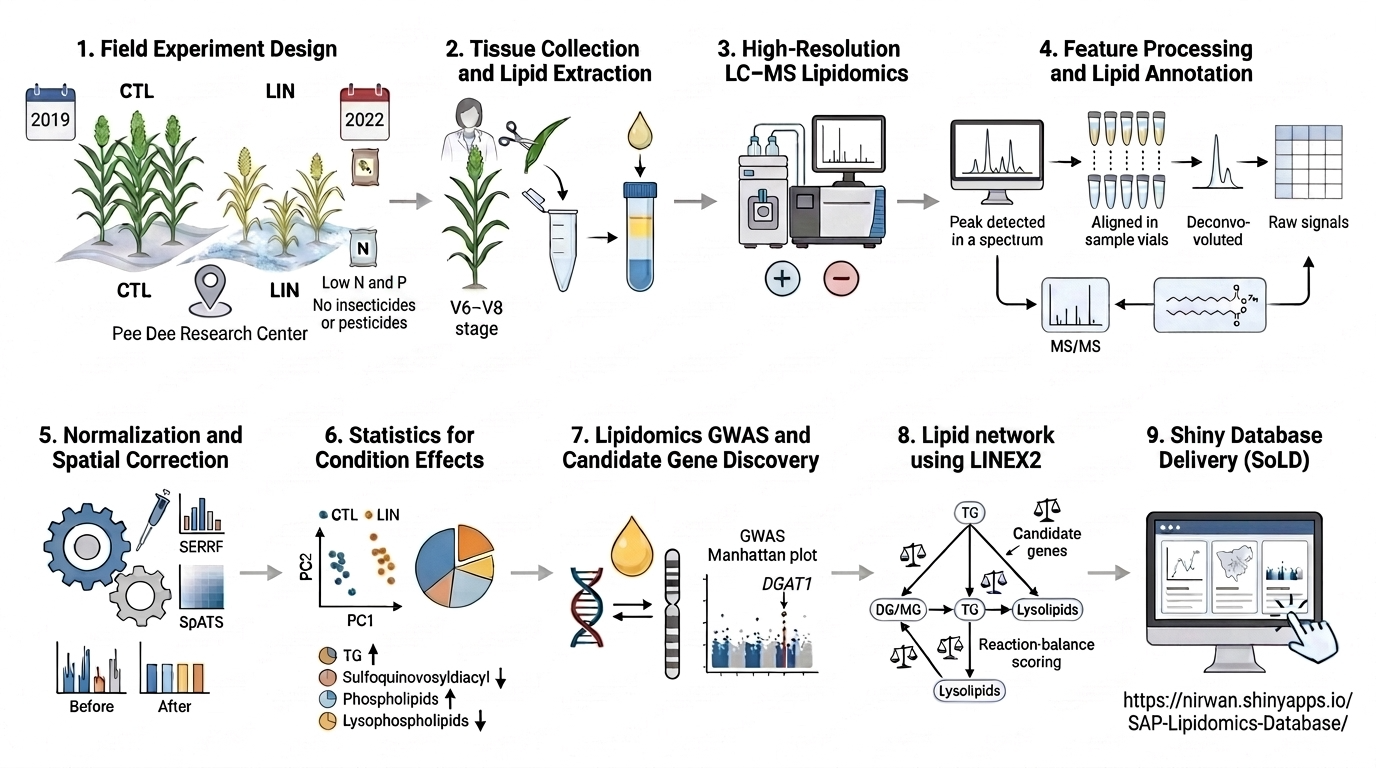
\includegraphics[width=\textwidth]{fig/supp/SuppFig_S1_Workflow.png}
\caption{\textbf{Field-to-database workflow.} Sample collection and lipid
extraction, high-resolution LC-MS lipidomic profiling, GNPS-assisted feature
processing and annotation, post-acquisition correction with SERRF and SpATS,
statistical description of each trial, lipidomics GWAS and candidate gene
discovery, LINEX2 reaction mapping, and dissemination through the SoLD Shiny
application.}
\label{fig:suppfig_s1_workflow}
\end{figure*}

\begin{figure*}[!ht]
\centering
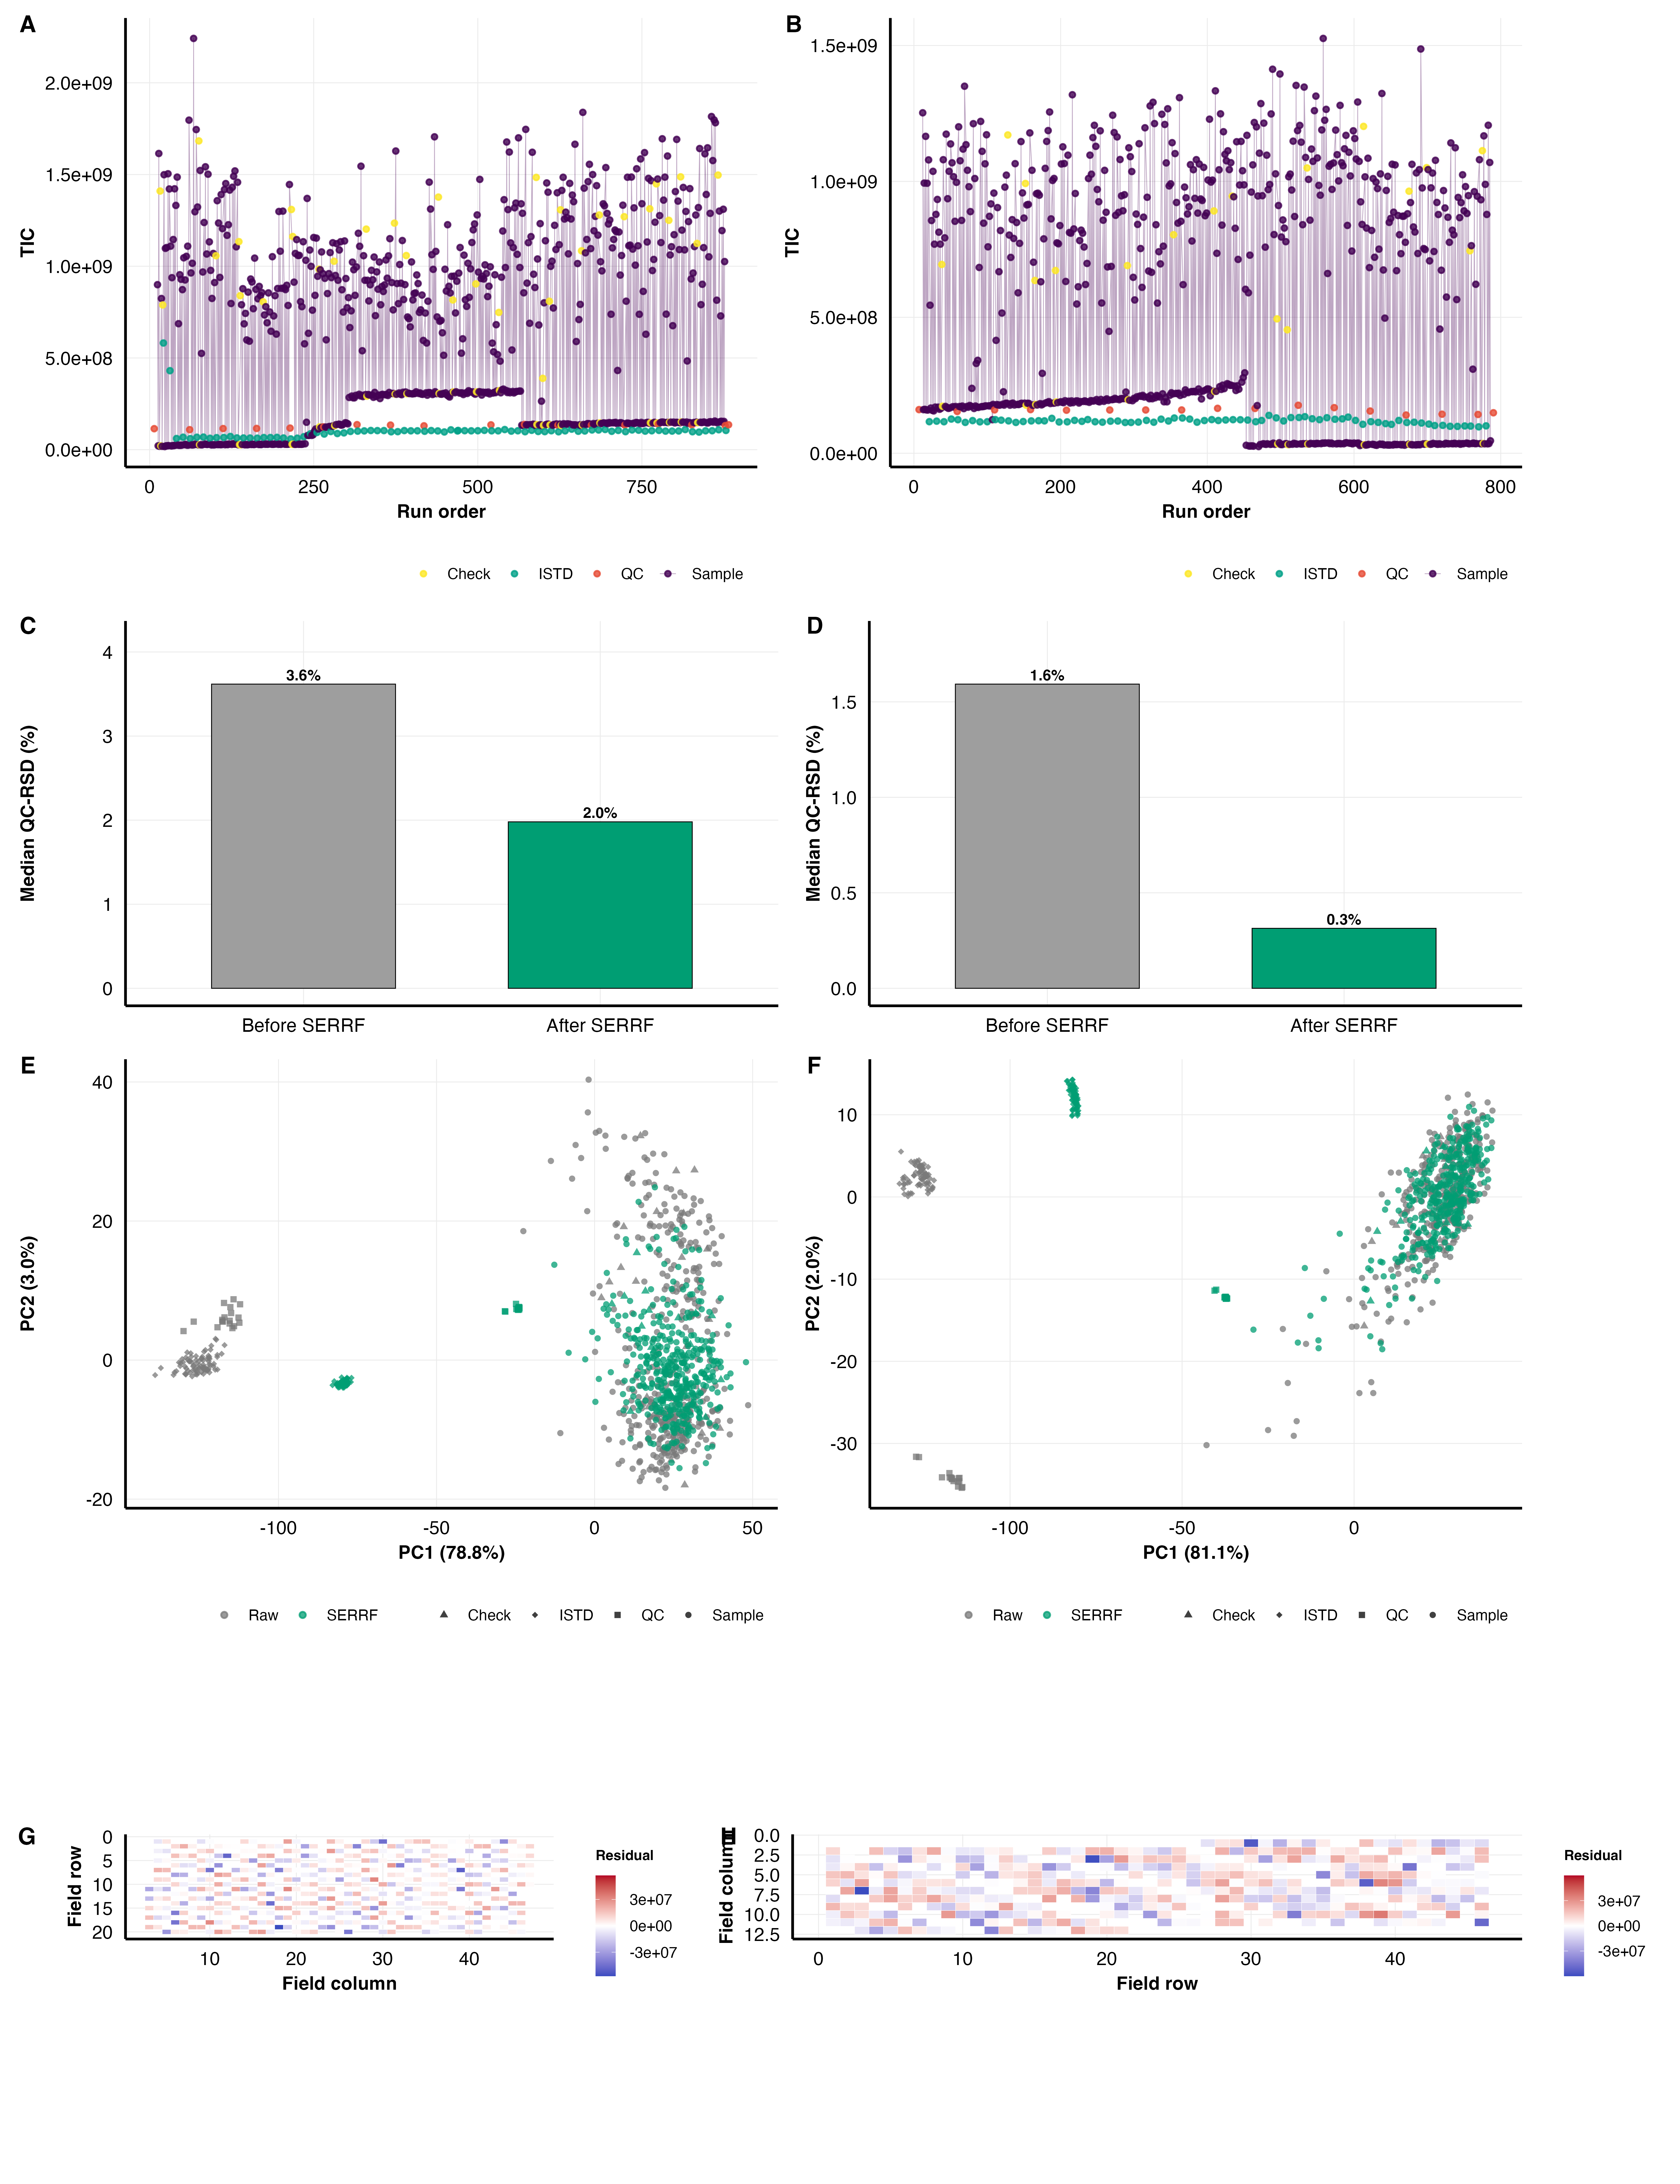
\includegraphics[width=\textwidth]{fig/supp/SuppFig_S2_QC_RunOrder_SERRF_PCA_SpATS.png}
\caption{\textbf{Quality control, SERRF normalization, and SpATS spatial adjustment diagnostics.}
(A,B) Run-order TIC plots for CTL and LIN conditions demonstrating stable analytical performance throughout the acquisition sequence.
(C,D) QC-RSD distributions before and after SERRF normalization, showing reduction in technical variation.
(E,F) PCA score plots comparing sample clustering before and after normalization.
(G,H) SpATS spatial residual maps indicating successful mitigation of field-position effects in both conditions.}
\label{fig:suppfig_s2_qc}
\end{figure*}

\begin{figure*}[!ht]
\centering
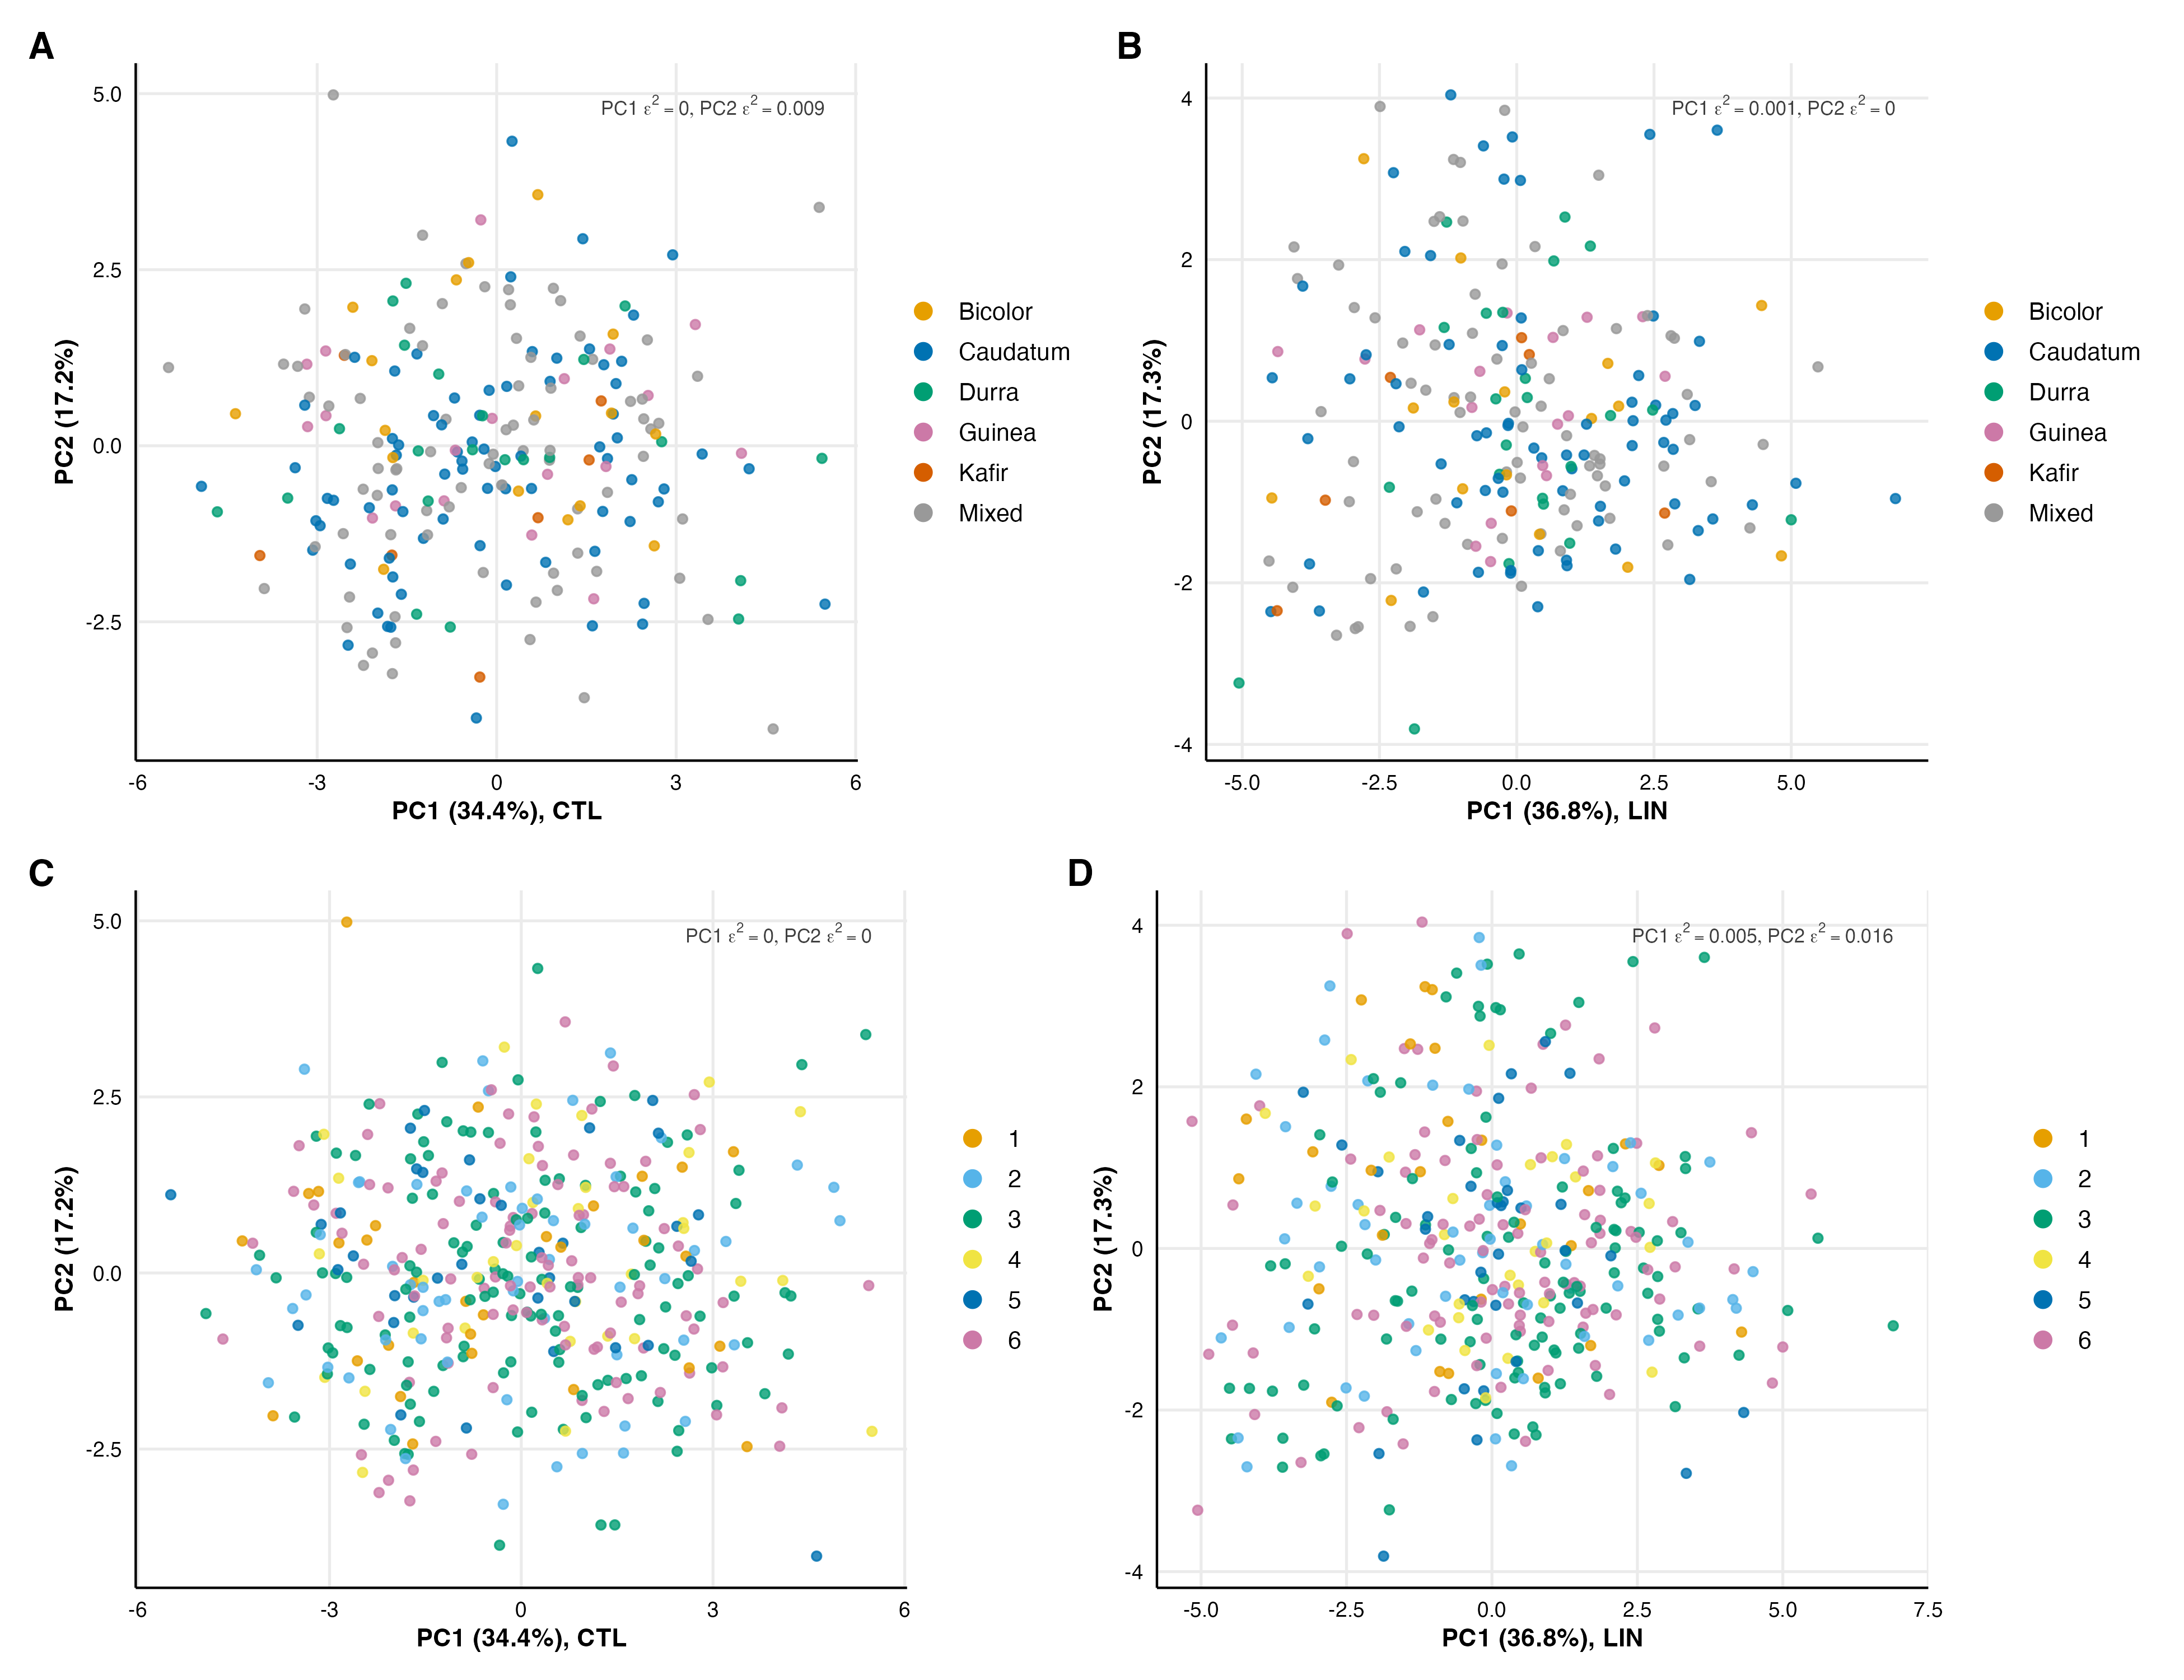
\includegraphics[width=\textwidth]{fig/supp/SuppFig_S3_Class_PCA_Structure.png}
\caption{\textbf{Lipid-class composition does not separate accessions by botanical
race or by genetic cluster.} Principal component analysis of the 13 lipid-class
percentages, run separately within each field trial on log$_{10}$ values scaled to
unit variance so that no single dominant class sets the axes.
\textbf{(A,B)}~Accessions coloured by botanical race in CTL and LIN.
\textbf{(C,D)}~The same two ordinations coloured by marker-based genetic cluster
($K=6$). Each panel gives the variance in PC1 and PC2 explained by that grouping
($\varepsilon^2$, Kruskal--Wallis). No grouping explains either leading axis in
either trial.}
\label{fig:suppfig_s3_class_pca}
\end{figure*}

\begin{figure*}[!ht]
\centering
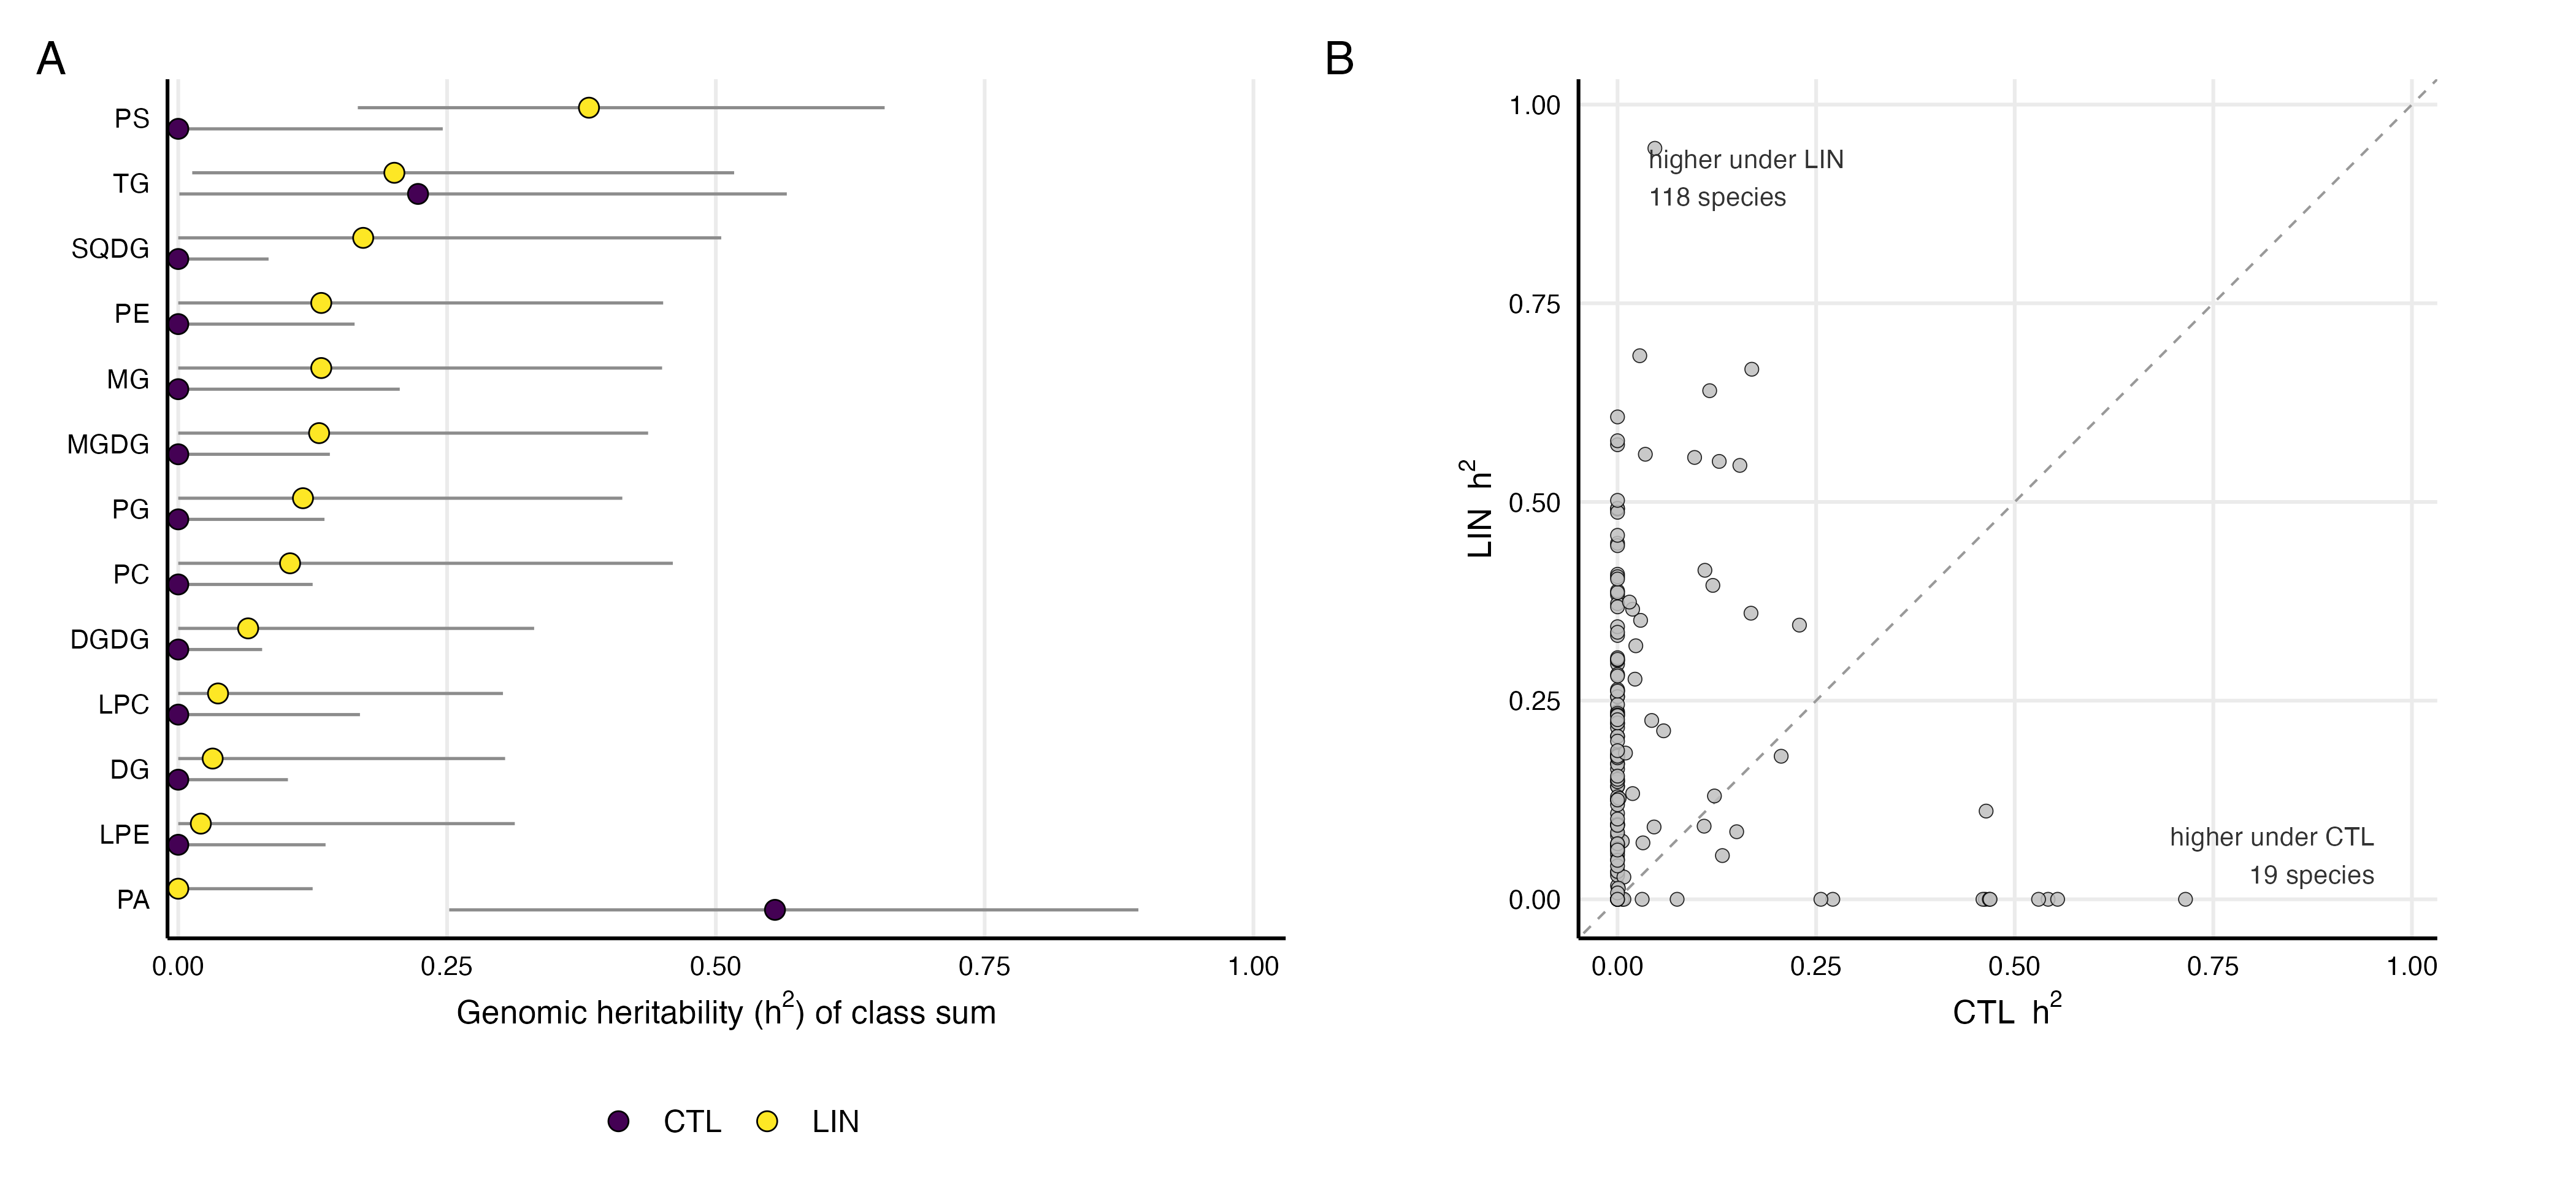
\includegraphics[width=\textwidth]{fig/supp/SuppFig_S4_Heritability.png}
\caption{\textbf{Genomic heritability of lipid traits in the two field trials.}
\textbf{(A)}~Genomic heritability of each of the 17 lipid-class sums, point
estimate with its 95\% profile-likelihood interval, on every accession of the
trial that is in the relationship matrix (389 under CTL, 357 under LIN) and
every species of that class detected in that trial. \textbf{(B)}~Paired
per-species heritability, one point per species, CTL on the horizontal axis and
LIN on the vertical; the dashed line is equality. Panel~B is restricted to the
same 351 genotypes and the same 163 species detected in both trials, so there
the two trials differ only in the phenotype measured. Both panels use the same
genomic relationship matrix and the same $\log_{10}$ scale.}
\label{fig:suppfig_s4_heritability}
\end{figure*}

\begin{figure*}[!ht]
\centering
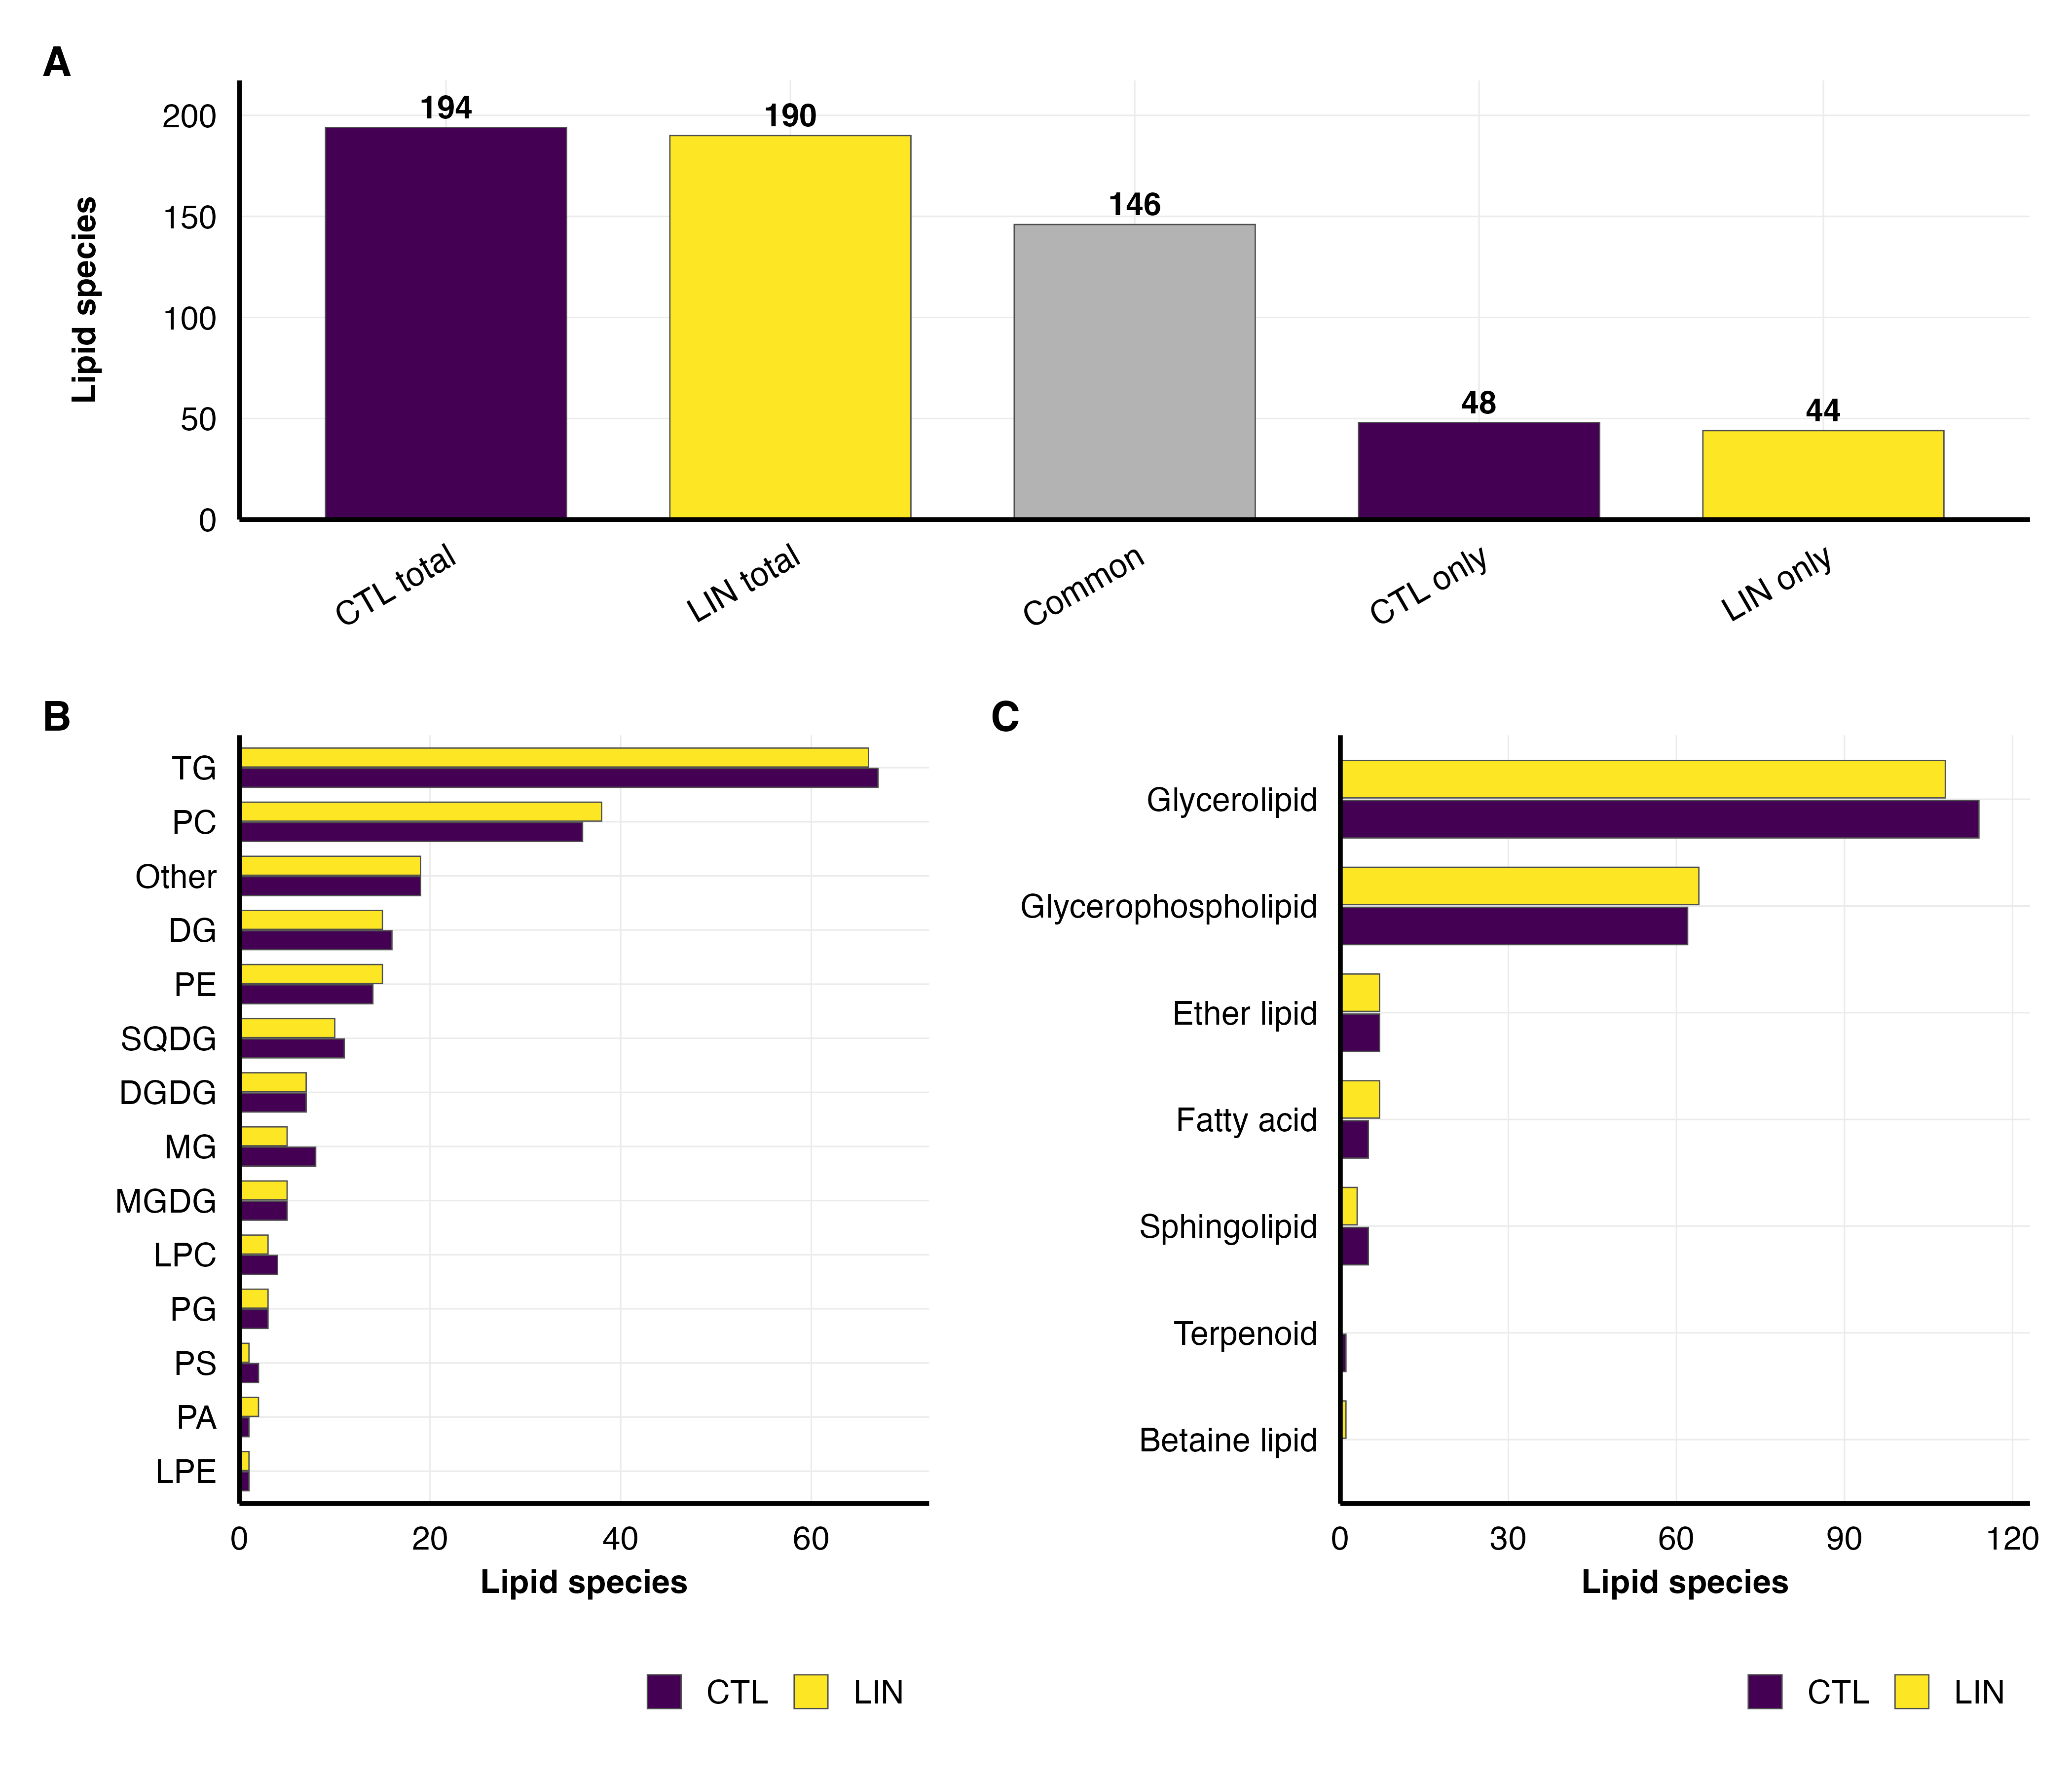
\includegraphics[width=\textwidth]{fig/supp/SuppFig_S5_Lipid_Species_Counts.png}
\caption{\textbf{Lipid species counts and overlap between conditions.}
\textbf{(A)}~Species detected in each trial, with the common and trial-specific counts.
\textbf{(B)}~Counts by lipid class. \textbf{(C)}~Counts by LIPID MAPS category. Counts
cover features annotated in lipid shorthand notation; the carotenoids, sterols,
tocopherols, quinones and free sphingoid bases carried under trivial names are
excluded here but retained in the composition analyses.}
\label{fig:suppfig_s5_counts}
\end{figure*}

\begin{figure*}[!ht]
\centering
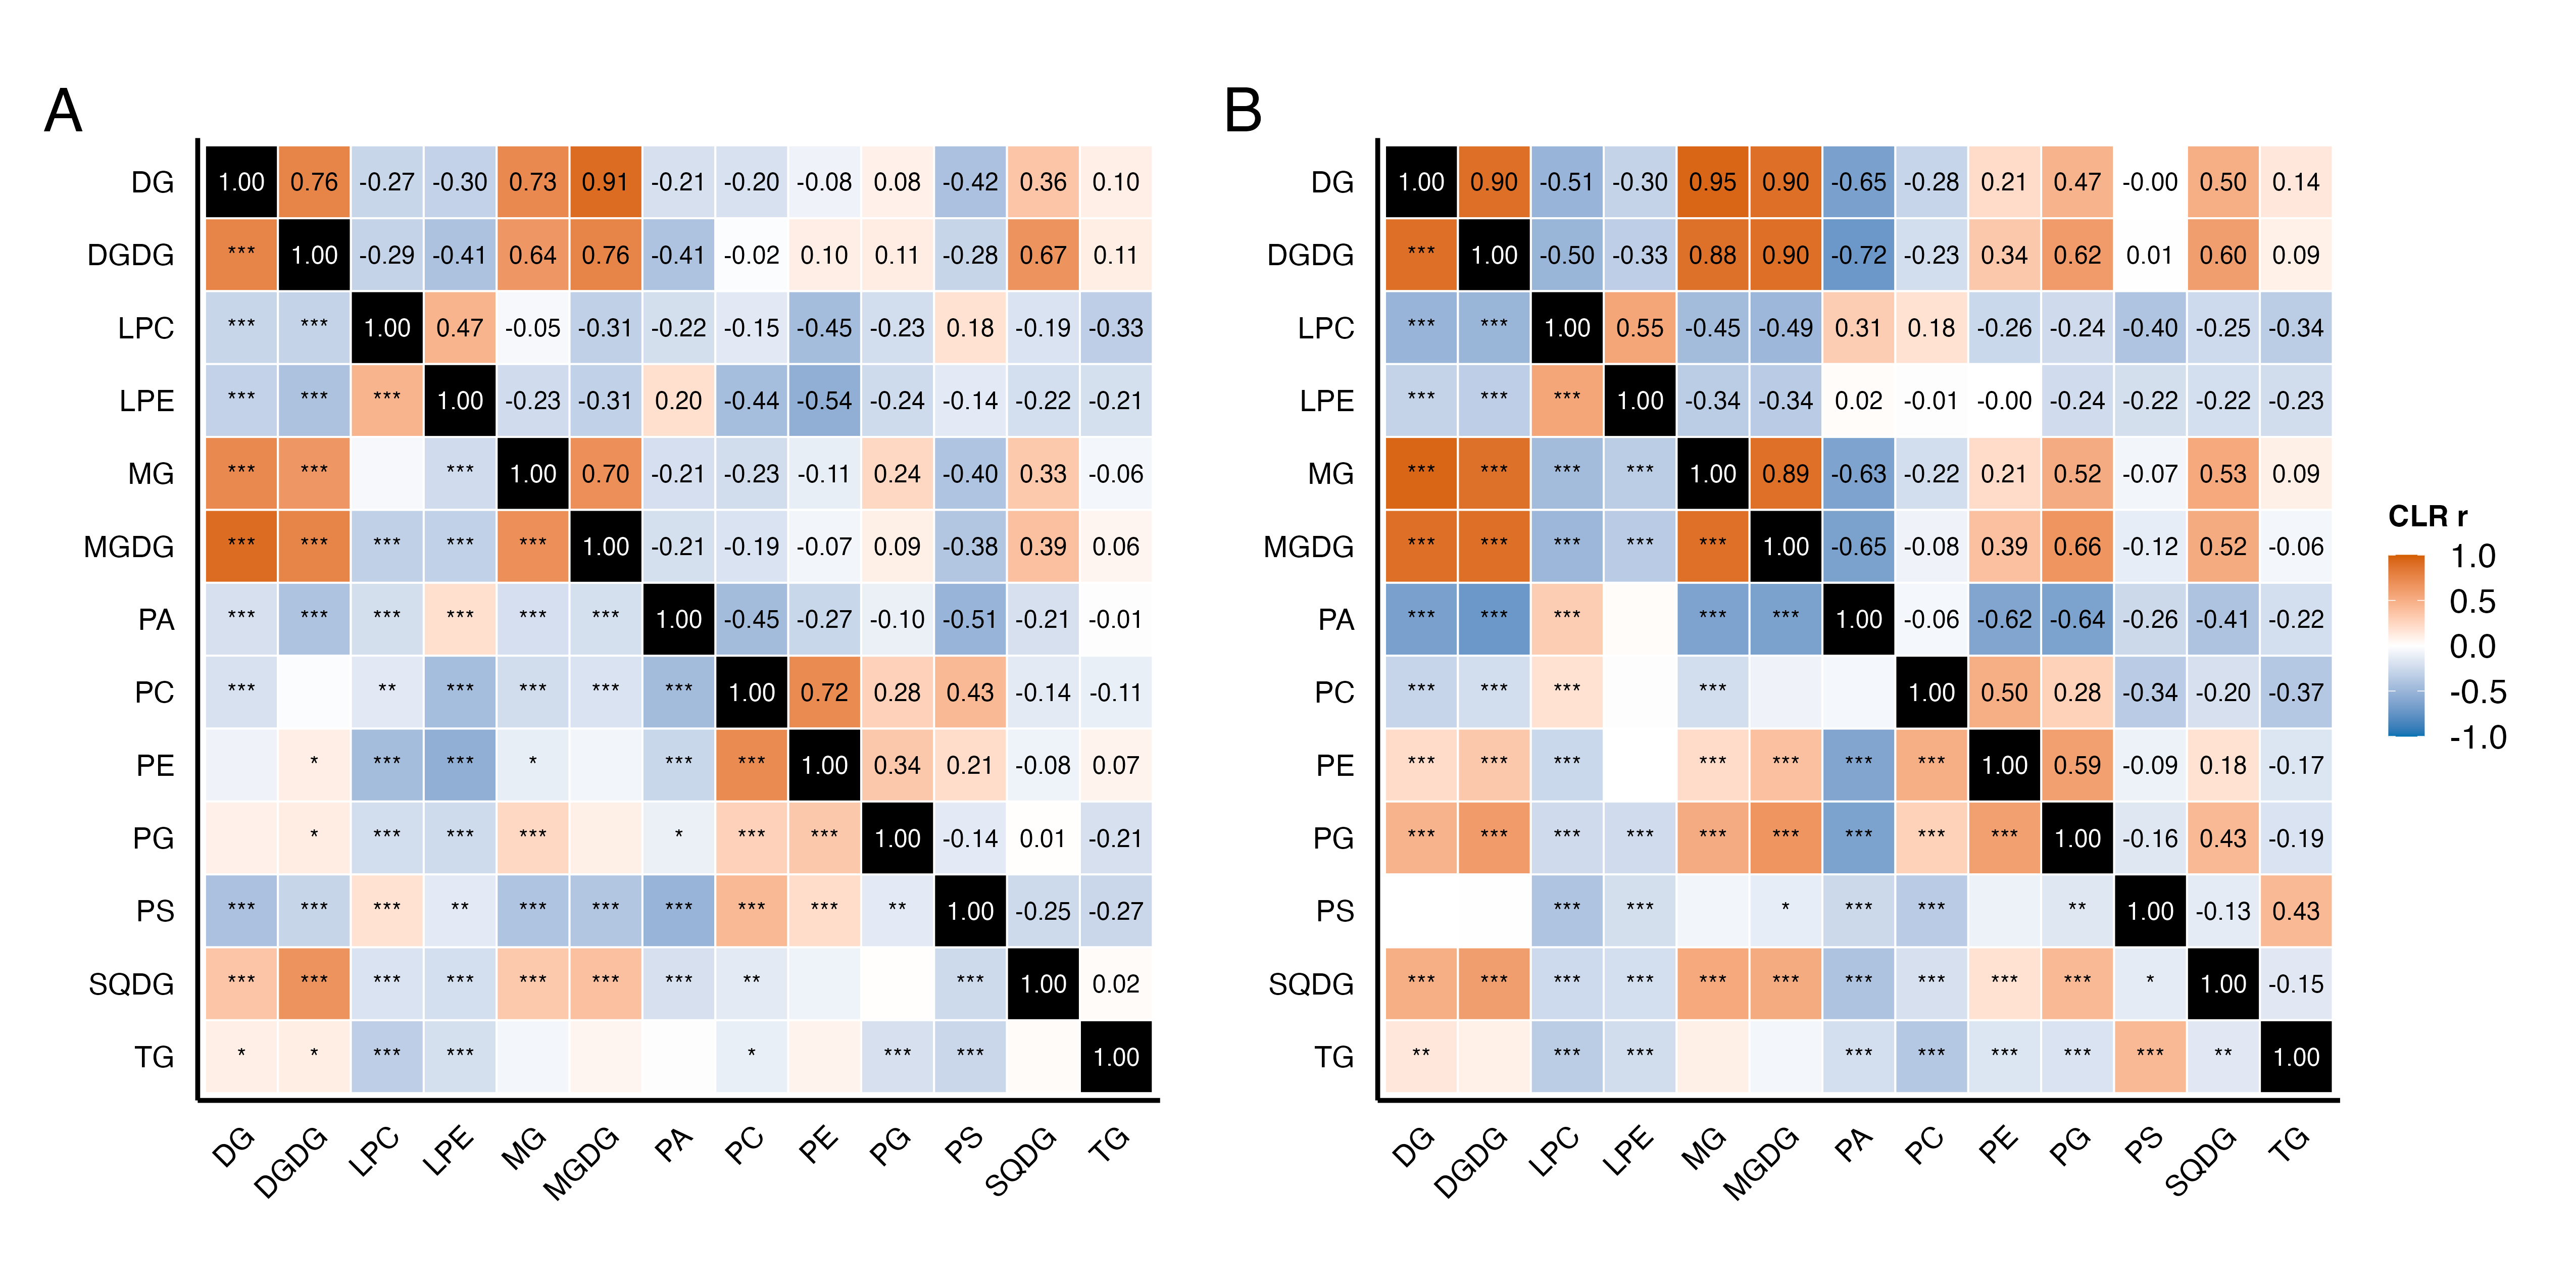
\includegraphics[width=\textwidth]{fig/supp/SuppFig_S6_CLR_Correlations.png}
\caption{\textbf{Correlation structure among lipid classes within each field
trial.} Pearson correlation matrices computed on class-level centered log-ratio
abundances for \textbf{(A)}~CTL and \textbf{(B)}~LIN. The lower triangle gives
the correlation coefficient and the upper triangle its significance
(*$p<0.05$, **$p<0.01$, ***$p<0.001$). Each matrix is computed within one trial
and the two are not differenced.}
\label{fig:suppfig_s6_pcor}
\end{figure*}

\begin{figure*}[!ht]
\centering
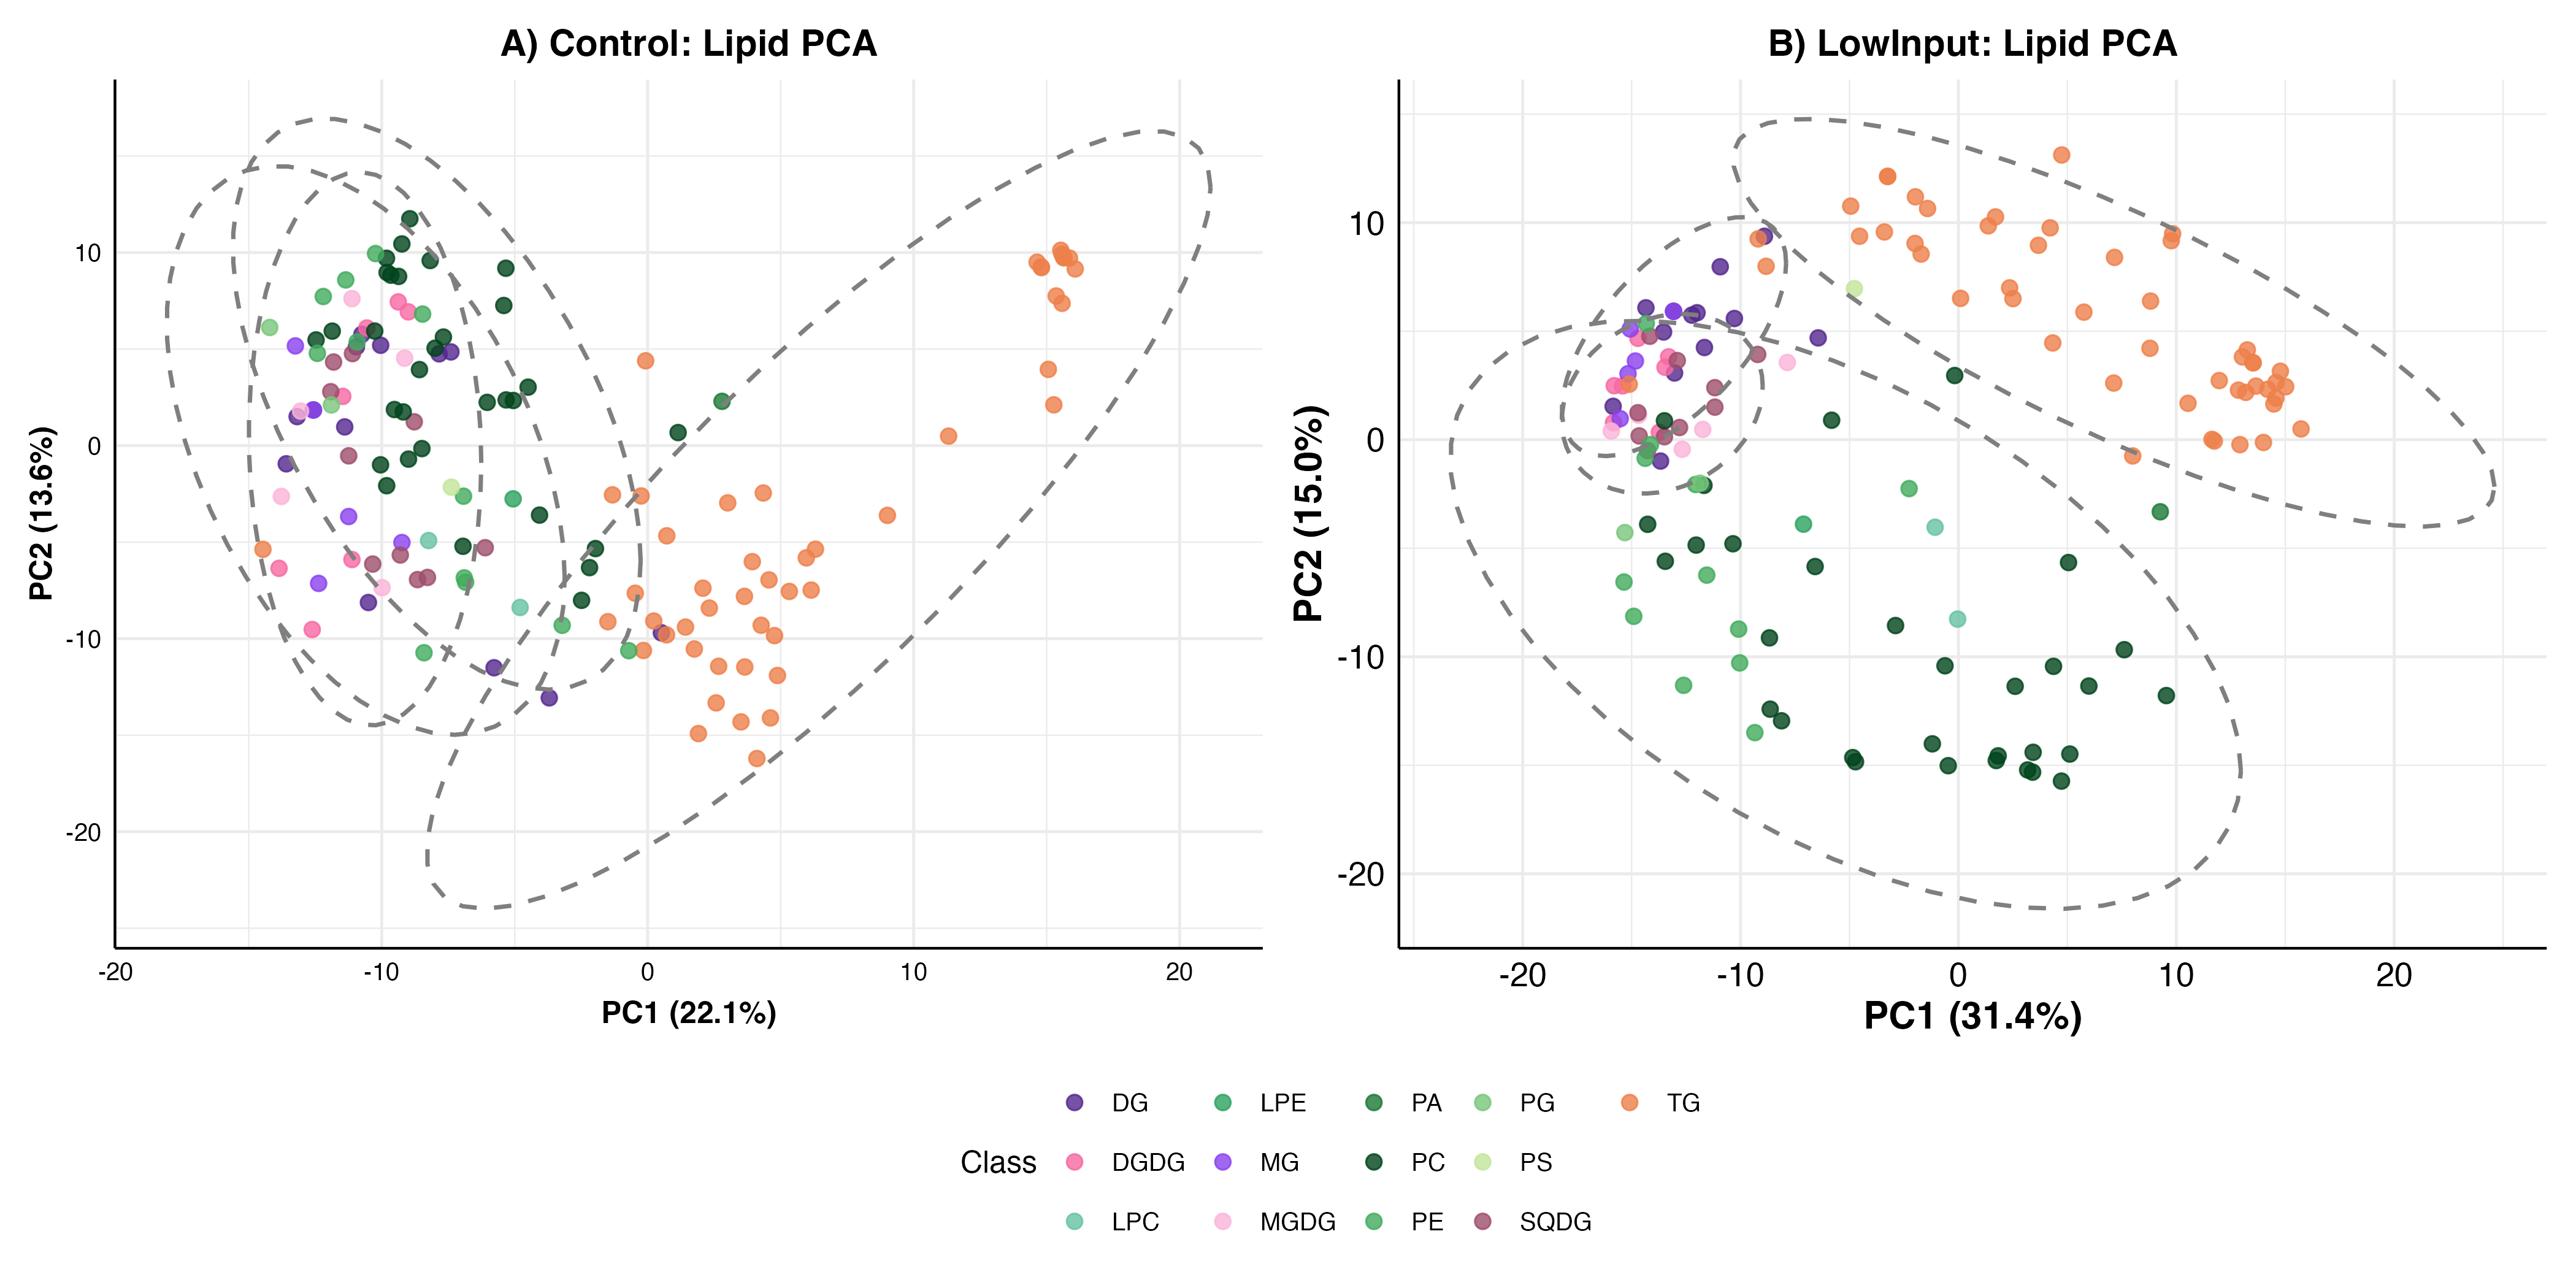
\includegraphics[width=\textwidth]{fig/supp/SuppFig_S7_PCA_Lipids.png}
\caption{\textbf{PCA of lipid species in compositional space.}
(A) PCA score plot of CLR-transformed lipid species in CTL samples, with 95\% confidence ellipses for LIPID MAPS category groups.
(B) PCA score plot for LIN samples using the same transformation. Points are colored by lipid class.}
\label{fig:suppfig_s7_pca}
\end{figure*}

\begin{figure*}[!ht]
\centering
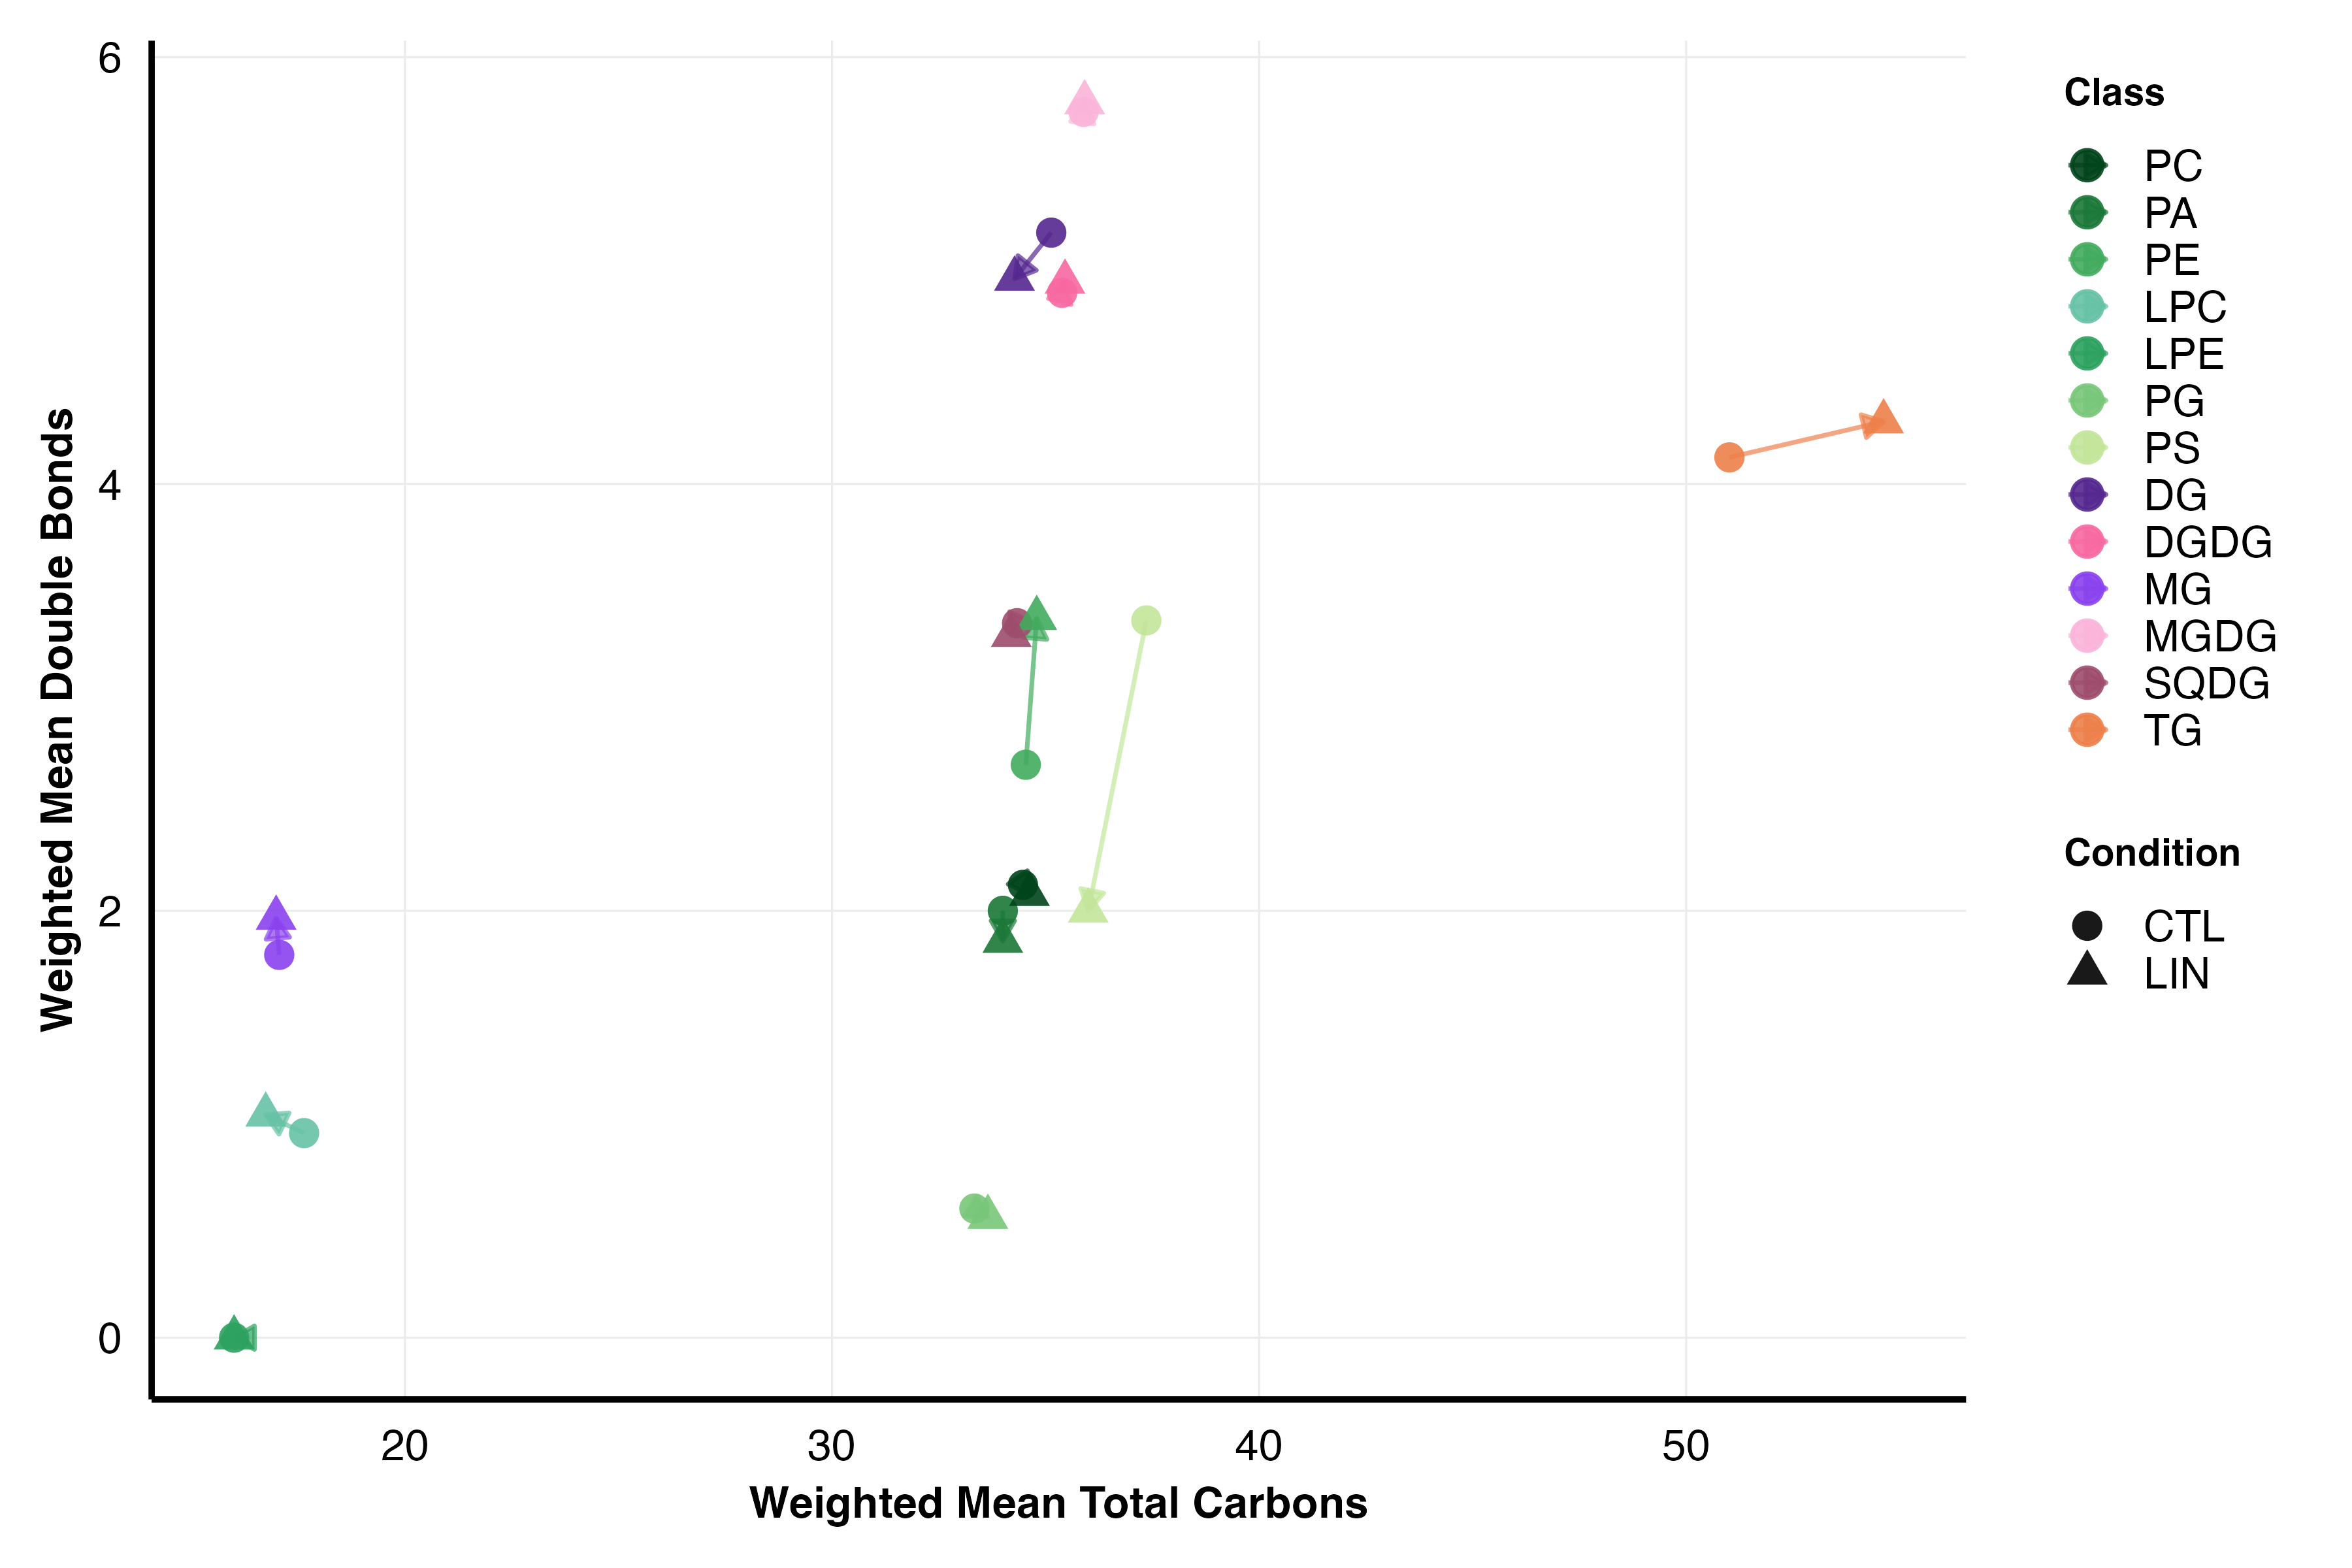
\includegraphics[width=0.9\textwidth]{fig/supp/SuppFig_S8_Chemical_Space.png}
\caption{\textbf{Lipid classes in a reduced chemical space.} Each point is one
lipid class, placed at its abundance-weighted mean total carbon number and its
abundance-weighted mean double-bond count across the species it contains, with
the weights taken from the \%TIC composition. Colour gives the class and shape
the trial, and the arrow runs from a class's CTL position to its LIN position.
The two trials differ in year, field and acquisition batch, so these shifts are
descriptive. Classes represented by one to three species (PS, PA, LPE, PG) have
unstable positions, because the species detected in the two trials are not the
same; the PS shift, for example, follows the loss of PS(18:0/20:4) from the
detected set rather than remodelling of a PS pool.}
\label{fig:suppfig_s8_chem}
\end{figure*}











\begin{figure*}[!ht]
\centering
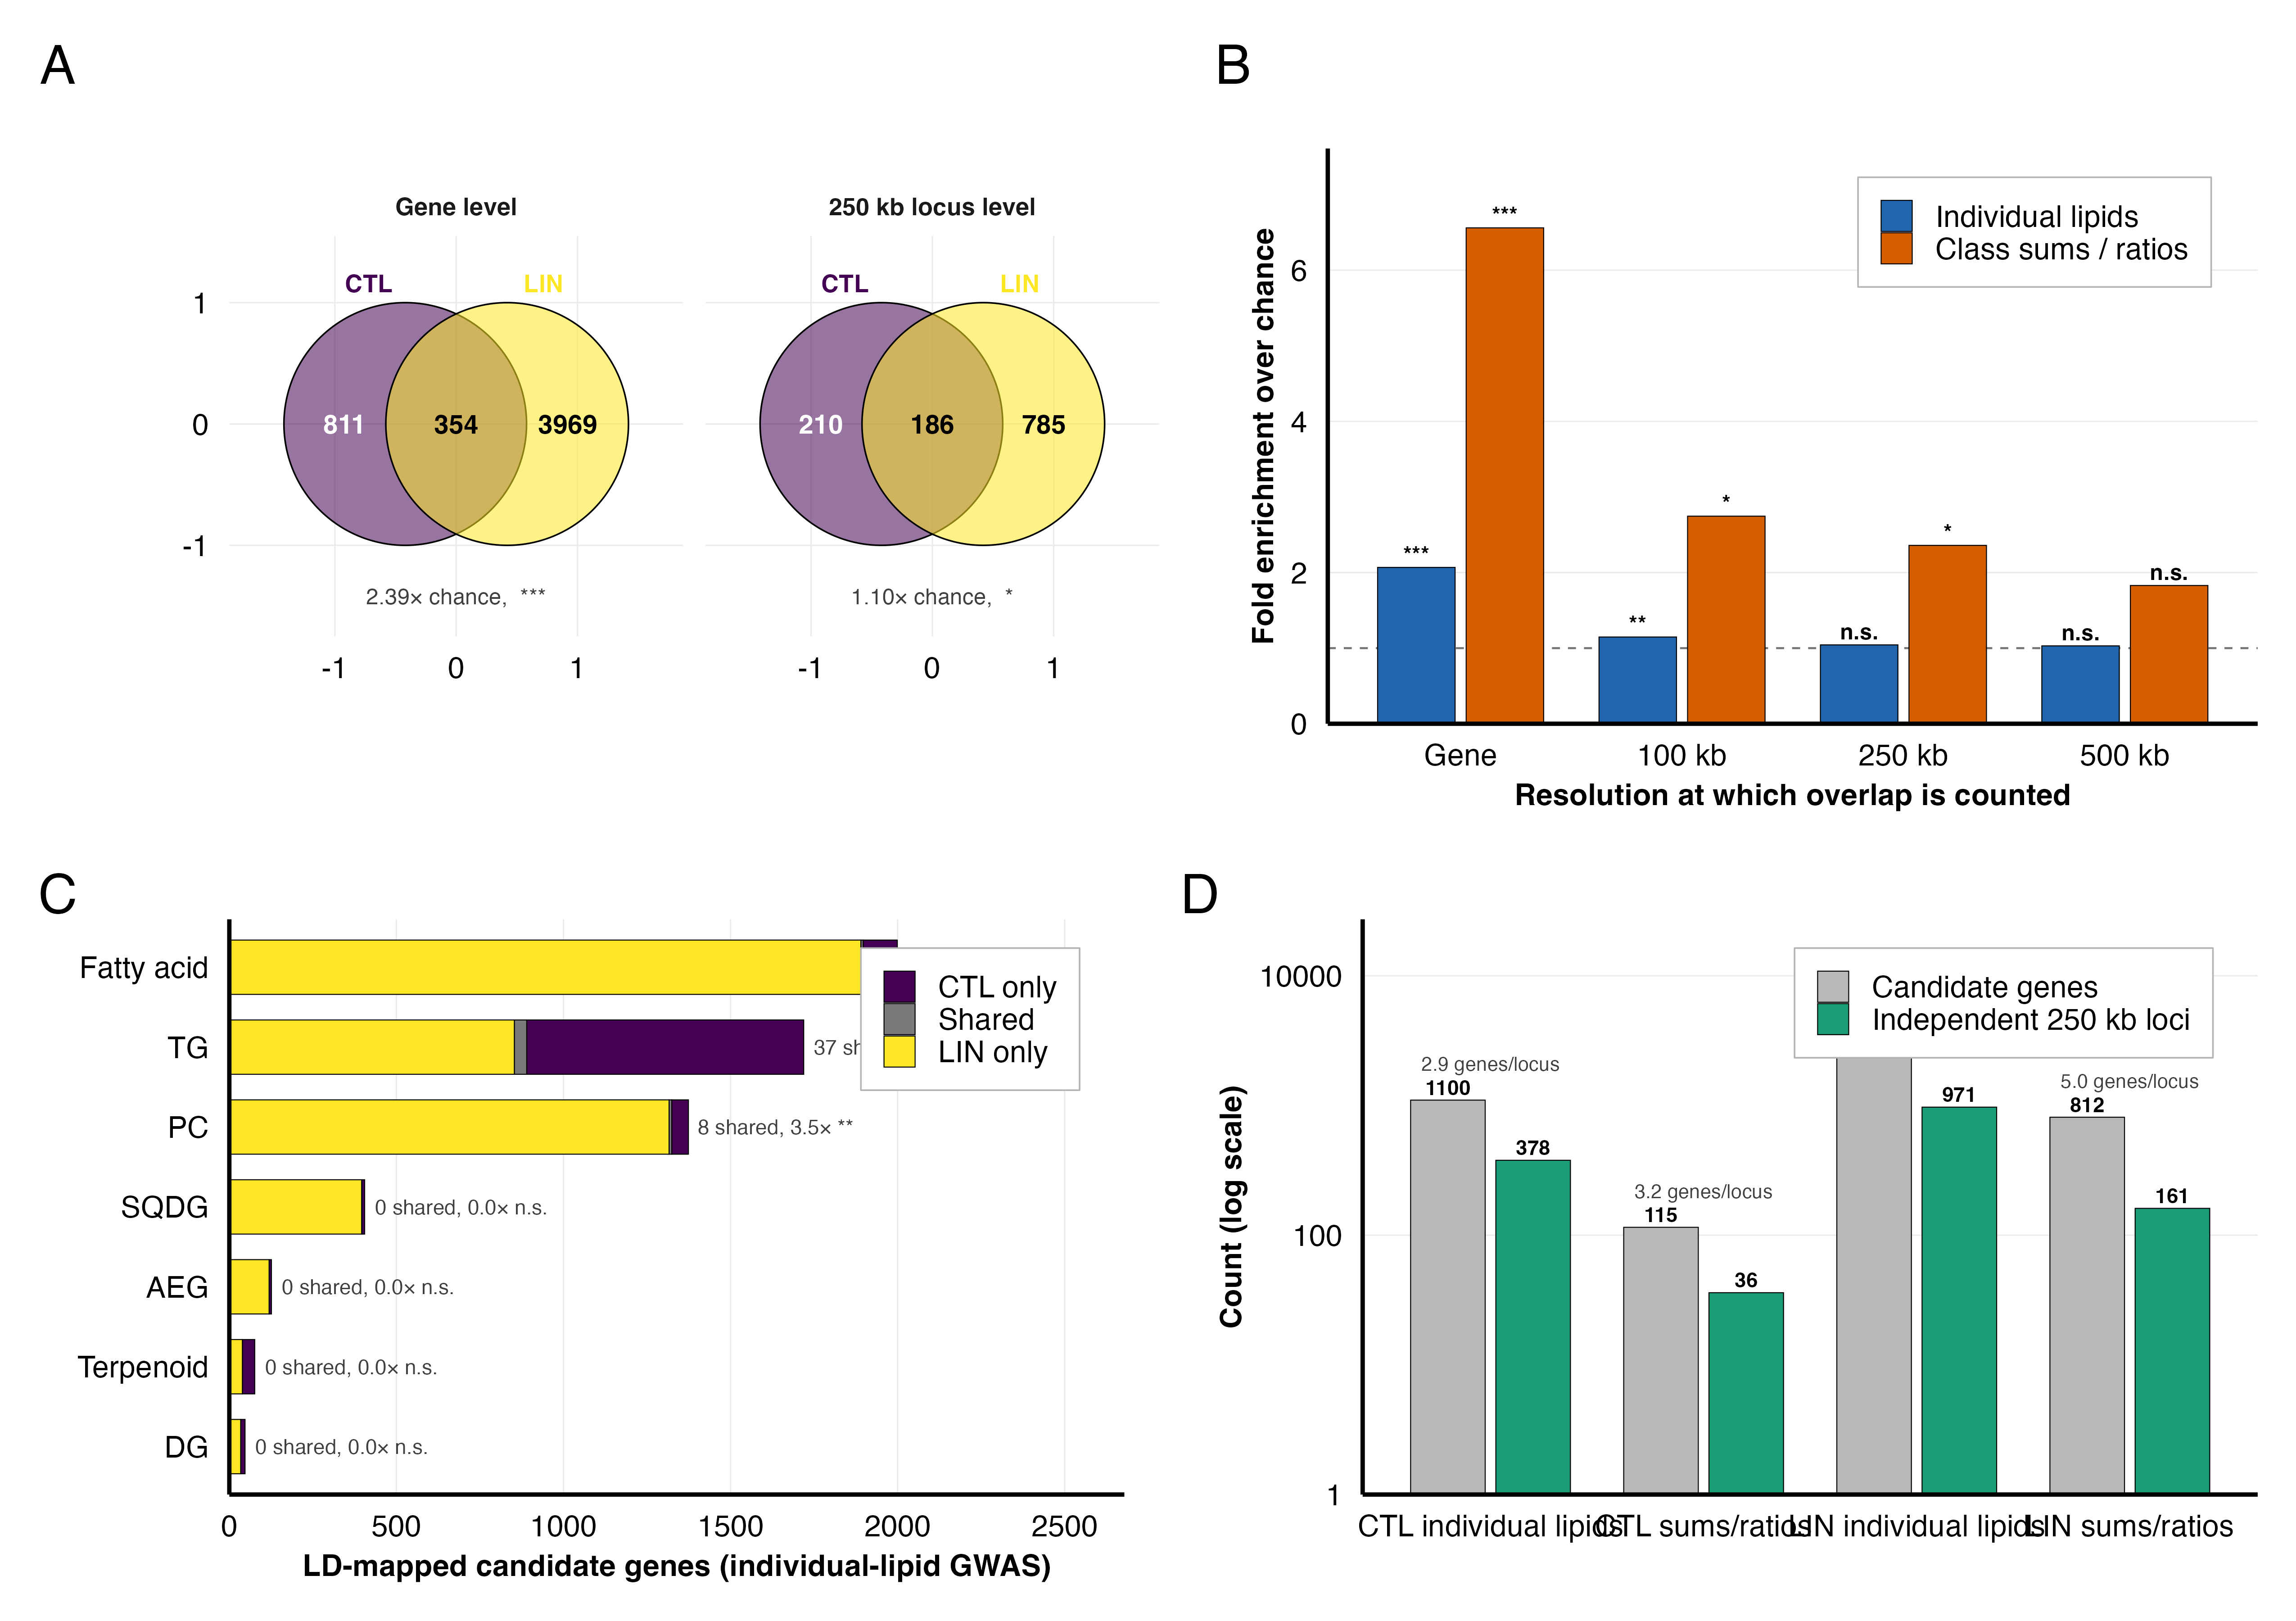
\includegraphics[width=\textwidth]{fig/supp/Figure7_CTL_LIN_Overlap.png}
\caption{\textbf{CTL and LIN GWAS identify largely non-overlapping candidate loci.}
(A) Overlap of candidate sets at gene level and after collapsing linkage blocks into 250~kb loci, with fold enrichment over chance and hypergeometric $P$.
(B) Fold enrichment of the overlap as a function of the resolution at which it is counted, for individual-lipid and class-sum/ratio traits. The dashed line marks chance expectation; *** $P<0.001$, ** $P<0.01$, * $P<0.05$, n.s., not significant.
(C) Candidate genes per lipid class in the individual-lipid GWAS, partitioned into CTL-only, shared, and LIN-only.
(D) Candidate-gene counts compared with the number of independent 250~kb loci they occupy (log scale).}
\label{fig:fig7_ctl_lin_overlap}
\end{figure*}


% Supplementary tables are supplied as separate supporting-information files
% (table/supp/ in the repository), not typeset here. Cited in the text as
% Supplementary Table~S4, S3, S7 and so on.

\end{document}
